\documentclass[12pt]{report}

\usepackage[utf8]{inputenc}
\usepackage[spanish, english]{babel}
\usepackage{graphicx}
\usepackage{amssymb, amsmath, amsthm}
\usepackage{bm} % For boldface greek letters
\usepackage{hyperref} % Para poder tener hyperlinks
\usepackage{enumerate}
\usepackage{calligra} % Para dedicacion
\usepackage[sorting=none]{biblatex}
\addbibresource{library.bib}
\usepackage{csquotes}


%%%%%% Mis Codigos

% TODO notes package
\usepackage{xargs}                  % Use more than one optional parameter in a new command
\usepackage[pdftex,dvipsnames]{xcolor}
%\usepackage{xargs}                      % Use more than one optional parameter in a new
%\usepackage[pdftex,dvipsnames]{xcolor}  % Coloured text etc.

%
%\usepackage[colorinlistoftodos,prependcaption,textsize=tiny]{todonotes}
\usepackage{todonotes}

\newcommandx{\unsure}[2][1=]{\todo[linecolor=red,backgroundcolor=red!25,bordercolor=red,#1]{#2}}
\newcommandx{\change}[2][1=]{\todo[linecolor=blue,backgroundcolor=blue!25,bordercolor=blue,#1]{#2}}
\newcommandx{\complete}[2][1=]{\todo[linecolor=pink,backgroundcolor=pink!25,bordercolor=blue,#1]{#2}}
\newcommandx{\info}[2][1=]{\todo[linecolor=OliveGreen,backgroundcolor=OliveGreen!25,bordercolor=OliveGreen,#1]{#2}}
\newcommandx{\improvement}[2][1=]{\todo[linecolor=Plum,backgroundcolor=Plum!25,bordercolor=Plum,#1]{#2}}
\newcommandx{\thiswillnotshow}[2][1=]{\todo[disable,#1]{#2}}

% Colored text and boxes with my color conventions for highlighting
\usepackage[dvipsnames]{xcolor}
%\usepackage[dvipsnames]{xcolor}

%
% \newcommand{\ytext}[1]{\textcolor{yellow}{#1}}
% \newcommand{\otext}[1]{\textcolor{orange}{#1}}
% \newcommand{\rtext}[1]{\textcolor{red}{#1}}
% \newcommand{\lbtext}[1]{\textcolor{cyan}{#1}}
% \newcommand{\dbtext}[1]{\textcolor{blue}{#1}}
% \newcommand{\ptext}[1]{\textcolor{Plum}{#1}}
% \newcommand{\lgtext}[1]{\textcolor{LimeGreen}{#1}}
% \newcommand{\dgtext}[1]{\textcolor{OliveGreen}{#1}}

\newcommand{\ytext}[1]{\textcolor{black}{#1}}
\newcommand{\otext}[1]{\textcolor{black}{#1}}
\newcommand{\rtext}[1]{{\it #1}}
\newcommand{\lbtext}[1]{\textcolor{black}{#1}}
\newcommand{\dbtext}[1]{\textcolor{black}{#1}}
\newcommand{\ptext}[1]{\textcolor{black}{#1}}
\newcommand{\lgtext}[1]{\textcolor{black}{#1}}
\newcommand{\dgtext}[1]{\textcolor{black}{#1}}

% \newcommand{\ybox}[1]{\colorbox{yellow}{#1}}
% \newcommand{\obox}[1]{\colorbox{orange}{#1}}
% \newcommand{\rbox}[1]{\colorbox{Salmon}{#1}}
% \newcommand{\lbbox}[1]{\colorbox{SkyBlue}{#1}}
% \newcommand{\dbbox}[1]{\colorbox{NavyBlue}{#1}}
% \newcommand{\pbox}[1]{\colorbox{Plum}{#1}}
% \newcommand{\lgbox}[1]{\colorbox{LimeGreen}{#1}}
% \newcommand{\dgbox}[1]{\colorbox{OliveGreen}{#1}}

% Math symbols
\usepackage{xparse}

%\usepackage{amssymb,amsmath,amsthm}
%\usepackage{xparse}

%%% Common symbols redifined
\let\oldepsilon\epsilon
\renewcommand{\epsilon}{\varepsilon}
\renewcommand{\varepsilon}{\oldepsilon}

\let\oldphi\phi
\renewcommand{\phi}{\varphi}
\renewcommand{\varphi}{\oldphi}

\newcommand{\emty}{\varnothing}
\newcommand{\varempty}{\nothing}

%%% Common Sets
\newcommand{\bb}[1]{\ensuremath{\mathbb{#1}} }
\newcommand{\ZZ}{\ensuremath{\mathbb{Z}} }
\newcommand{\NN}{\ensuremath{\mathbb{N}} }
\newcommand{\QQ}{\ensuremath{\mathbb{Q}} }
\newcommand{\RR}{\ensuremath{\mathbb{R}} }
\newcommand{\CC}{\ensuremath{\mathbb{C}} }


\newcommand{\iss}{\cong}  % Isomorphism symbol, here it is the one with a tilde

%%%%%%%%%%%%%% Sets

\newcommand{\set}[1]{\ensuremath{\left\{ #1 \right\}}} % Set function, simply puts nice left and right braces
\newcommand{\st}{\ensuremath{\ |\ }} % Such that symbol, TODO improve

\newcommand{\psubset}{\ensuremath{\subset}}
\renewcommand{\subset}{\ensuremath{\subseteq}} % Subset symbol, in this case it is the subset or equal to symbol

\newcommand{\bunion}{\bigcup}
%\newcommand{\biun}{\bun^{\infty}}
%\newcommand{\bfun}[3][n]{\bun_{#1 = #2}^{#3}}
\newcommand{\union}{\cup}
%\newcommand{\siun}{\sun^{\infty}}
%\newcommand{\sfun}[3][n]{\sun_{#1 = #2}^{#3}}

\newcommand{\binter}{\bigcap}
%\newcommand{\biinter}{\binter^{\infty}}
%\newcommand{\bfifter}[3][n]{\binter_{#1 = #2}^{#3}}
\newcommand{\inter}{\cap}
%\newcommand{\sininter}{\sinter^{\infty}}
%\newcommand{\sfinter}[3][n]{\sinter_{#1 = #2}^{#3}}

%%%%%% Calculus

% Integrals

%% Single Integrals
\NewDocumentCommand \integ {s O{} O{} m o}
{
	\IfBooleanTF{#1}{\oint}{\int}_{#2}^{#3} #4 %
	\IfNoValueF {#5} {\mathrm{d} #5}
}

%% Derivatives

% Normal derivative
% Example: \der[n]{f}{x}[x_0]
\NewDocumentCommand \der {O{} m m o}
{
	\frac{\mathrm{d}^{#1} #2}{\mathrm{d} {#3}^{#1}}%
	\IfNoValueF{#4} {\biggr|_{#4}}
}

%% Partial Derivatives

% With respect to one variable
% Example: \pder[n]{f}{y}[\pthvars[x_0][y_0][z_0]][(x, z)
\NewDocumentCommand \pder {O{} m m O{} o}
{
    \ensuremath{
	\IfNoValueTF {#5}
	{
		\frac{\partial^{#1} #2}{\partial {#3}^{#1}} #4
	}
	{
		\left(%
		\frac{\partial^{#1} #2}{\partial {#3}^{#1}}%
		\right)_{#5}  #4
	}
	}
}

% With respecto to two variables
% Example: \twpder{g}{y}{x}[(x_0, y_0)]
\NewDocumentCommand \twpder {m m m O{}}
{
	\frac{\partial^2 #1}{\partial #2 \partial #3} #4
}

\newcommand{\abs}[1]{\left\lvert #1 \right\rvert}
\newcommand{\norm}[1]{\left\lVert #1 \right\rVert}

% Physics symbols (vectors, units)
%\usepackage{tikz}
%\input{tools/physics_macros}

% Theorem environments
%%Version of October 8, 2016

%\usepackage{amsthm}

\theoremstyle{definition} %To avoid the annoying italics all the time, and to not sloppily redefine all of them 

\newtheorem{theo}{Theorem}[section]  %numbered according to section environment, so in section to it restarts as 2.1 
\newtheorem{prop}{Proposition}[section]  %numbered according to section environment, so in section to it restarts as 2.1 
\newtheorem{lemma}[theo]{Lemma}     %numbering shared with theorem 
\newtheorem{defn}{Definition}[section]   
\newtheorem{coro}{Corollary}[theo]


\theoremstyle{remark} 
\newtheorem*{remark}{Remark} 
 
%\let\oldtheo\theo 
%\renewcommand{\theo}{\oldtheo\normalfont}  
%  
%\let\olddefn\defn  
%\renewcommand{\defn}{\olddefn\normalfont}  
%  
%\let\oldlemma\lemma  
%\renewcommand{\lemma}{\oldlemma\normalfont}  
%  
%\let\oldcoro\coro  
%\renewcommand{\coro}{\oldcoro\normalfont}

%%%%%%%% ``Example'' environment, very basic, doesnt work with itemize
\theoremstyle{definition}

\newtheorem*{exmp}{Example}

\usepackage{tikz-cd} %To do Commutative Diagrams

% Extras
\newcommand{\linea}{\rule{10cm}{1mm}}
\usepackage{ulem}
\renewcommand{\theequation}{\thechapter.\arabic{equation}} % To label Ch 0 equations as 0.1, 0.2, etc

%%%%%%%
\newenvironment{dedication}
  {\clearpage           % we want a new page
   \thispagestyle{empty}% no header and footer
   \vspace*{\stretch{1}}% some space at the top 
   \raggedleft          % flush to the right margin
  }
  {\par % end the paragraph
   \vspace{\stretch{3}} % space at bottom is three times that at the top
   \clearpage           % finish off the page
  }

%%%%%%%
\graphicspath{ {images/} }

%%%%%%%
\theoremstyle{definition}
\newtheorem{example}{Example}[section]
\newtheorem{definition}[example]{Definition}
\newtheorem{theorem}[example]{Theorem}
\newtheorem{proposition}[example]{Proposition}
\newtheorem{lemma}[example]{Lemma}
\newtheorem{corollary}[example]{Corollary}
\newtheorem{notation}[example]{Notation}
\newtheorem{remark}[example]{Remark}

\usepackage{environ}

\NewEnviron{eqnsplit}{%
  \begin{equation}
  \begin{split}
    \BODY
  \end{split}
  \end{equation}
}

\NewEnviron{eqnsplit*}{%
  \begin{equation*}
  \begin{split}
    \BODY
  \end{split}
  \end{equation*}
}
%%%%%%%

\DeclareMathOperator{\HH}{\bb H}
\DeclareMathOperator{\diffeo}{\cong}
\DeclareMathOperator{\tr}{tr}

\DeclareMathOperator{\Diff}{\textit{Diff}}
\DeclareMathOperator{\Hom}{\textit{Hom}}
\DeclareMathOperator{\End}{\textit{End}}


\newcommand{\algeb}[1]{\mathfrak{#1}}
\newcommand{\alg}[1]{\mathfrak{#1}}
\newcommand{\oid}[1]{\ensuremath{\mathfrak{#1}}}
\newcommand{\ppal}[1]{\ensuremath{\mathcal{#1}}}

\newcommand{\sect}[1]{\ensuremath{\bm{#1}}} % Boldface that affects greek letters
\newcommand{\sectalg}[1]{\sect{\alg{#1}}}
\newcommand{\sectoid}[1]{\sect{\oid{#1}}}
\newcommand{\sectppal}[1]{\sect{\ppal{#1}}}

\newcommand{\cl}[1]{\ensuremath{\left\langle #1 \right\rangle}}
\newcommand{\upsect}[1]{\overline{\sect{#1}}}
\newcommand{\downsect}[1]{\underline{\sect{#1}}}

\let\oldtilde\tilde
\renewcommand{\tilde}{\widetilde}
\newcommand{\stilde}[1]{\tilde{\sect{#1}}}

\DeclareMathOperator{\comp}{\circ}

%%%%%%%
\allowdisplaybreaks
\setlength{\parskip}{0.5em} % PARECE QUE NO ES USUAL DEJAR ESTE ESPACIO

\interfootnotelinepenalty=10000

\title 
{
	{Formulation and Generalization of Gauge Theories in the Language of Lie Algebroids}\\
	{\large Universidad de los Andes}\\
	\vspace{1.5cm}
	{
\includegraphics[width = 0.6\textwidth]{logo.png}}	
}
\author{Sebastian Camilo Puerto Galindo\\[1cm]{\small Advised by: Prof. Alexander Cardona Guio}}

%%%%%%%%%%%%%%%%%%%%%%%%%%%%%%%%%%%%%%%%%%%%%%%%%%%%%%%%%%%%%%%%%%%%%%%%%%%%%%
%%%%%%%%%%%%%%%%%%%%%%%%%%%%%%%%%%%%%%%%%%%%%%%%%%%%%%%%%%%%%%%%%%%%%%%%%%%%%%
%%%%%%%%%%%%%%%%%%%%%%%%%%%%%%%%%%%%%%%%%%%%%%%%%%%%%%%%%%%%%%%%%%%%%%%%%%%%%%
%%%%%%%%%%%%%%%%%%%%%%%%%%%%%%%%%%%%%%%%%%%%%%%%%%%%%%%%%%%%%%%%%%%%%%%%%%%%%%

\begin{document}

\pagenumbering{Roman}

\maketitle

\begin{dedication}
{\LARGE\calligra Hola}
\end{dedication}

\begin{abstract}
Hello
\end{abstract}

\begin{otherlanguage}{spanish}
\begin{abstract}
Hola
\end{abstract}
\end{otherlanguage}

\newpage

\chapter*{Acknowledgements}

\section*{English}
Hello
\begin{otherlanguage}{spanish}
\section*{Español}
Hola
\end{otherlanguage}

%%%%%%%%%%%%%%%%%%%%%%%%%%%%%%%%%%%%%%%%%%%%%%%%%%%%%%%%%%%%%%%%%%%%%%%%%%%%%%
%%%%%%%%%%%%%%%%%%%%%%%%%%%%%%%%%%%%%%%%%%%%%%%%%%%%%%%%%%%%%%%%%%%%%%%%%%%%%%
\tableofcontents

\pagenumbering{arabic}

%%%%%%%%%%%%%%%%%%%%%%%%%%%%%%%%%%%%%%%%%%%%%%%%%%%%%%%%%%%%%%%%%%%%%%%%%%%%%%
%%%%%%%%%%%%%%%%%%%%%%%%%%%%%%%%%%%%%%%%%%%%%%%%%%%%%%%%%%%%%%%%%%%%%%%%%%%%%%
\chapter*{Yet to Undertand}
%%%%%%%%%%%%%%%%%%%%%%%%%%%%%%%%%%%%%%%%%%%%%%%%%%%%%%%%%%%%%%%%%%%%%%%%%%%%%%%%%
\section{Crucial}
\begin{itemize}
    \item How important is the condition of good behaviour of the injection of $L$ after the connection applied to a fundamental field? Is it equivalent to removing the second basic condition in the definition of a ppal bundle connection?
    
    \item \rtext{Bosons?}
    
    \item The ordinary curvature is:
    \begin{itemize}
        \item The covariant derivative of $\omega$ with respecto to $\omega$, which can also be written as
        \item $d\omega(X_1^h, X_2^h)$
        \item $d\omega + \frac{1}{2}[\omega,\omega]$ (this $[,]$ is the Lie bracket of forms, not simplified notation).
        \item $\Omega^\omega = \omega + \omega \wedge \omega$ if $G$ is a matrix group.
    \end{itemize}
    
    \item Curvatures satisfy $2$ equations: Bianchi (or homogeneous field strength equation) and Another one (in the case of EM field $\delta F = 0$, which gives the conservation of charge), which talks about conservation.
    
    \item Why is ``field strenth'', i.e. curvature, a $2$-form?
    
    \item Perhaps the nice part of this language is the local trivializations where we see that ordinary connections do not act in any way in the second part: $\omega(X \oplus \gamma) = A(X) - \gamma$.
    
    \item Does our generalization of Connection give rise to a \rtext{truly covariant} derivative in ``associated vector bundles''?
    \begin{itemize}
        \item Perhaps induced by the fact that the covariant derivative in an associated vector bundle is precisely the covariant derivative of $E$-valued forms on $P$ seeing $\Gamma(E)$ as $0$-forms?
        
        \item \rtext{The covariant derivative of forms may also be defined as $D^\omega(\Omega)(X_1, \dots, X_m) = d\Omega(X_1^h, \dots, X_m^h)$}. The curvature is precisely the covariant derivative of $\omega$ wrt to $\omega$
        
        \item I read that ``covariant derivatives'' are equivalent to ordinary connections in $P$.
        
        \item Also, that the space of $G$-equivariant and horizontal $W$-valued $k$-forms on $P$ is equivalent to Space of $k$-forms on $M$ with values in $P\times_G W \to M$
        
        \item The covariant derivative of a \emph{basic}(horizontal and invariant) $k$-form may be written as: $D^\omega \tau = d\tau + \omega \dot{\wedge} \tau$ (See defn 1.3.4 and Thm 3.1.5 Bleecker) 
    \end{itemize}
    
    
    \item Ordinary connections give rise to a sense of horizontality both in $P$ AND in the associated vector bundles.
    
    \item What meaning may be given to
    \begin{itemize}
        \item The connection, instead of vertical projection
        
        \item The curvature, instead of $d\omega(X_1^h, X_2^h)$ (we still have: failure of $\omega$ to be ... morphism of Lie algebras?), perhaps specially in the ``associated'' bundles. Measure of \dbbox{integrability?}
        
        \item To the $\Theta:A \to A$, $\mathfrak X \mapsto \mathfrak X + i \comp \omega(\mathfrak X)$ 
        
        \item To $\hat \omega$, $\hat \Theta$, $\hat R$, $\hat F$?
        
        \item $L$: still the ``vertical part''?
    \end{itemize}
    
    \item Can we keep
    \begin{itemize}
        \item the property ``$\omega^2 = \omega$ ''? So that there is still a projection associated (without preserving $\omega |_L = -id_L$... it isn't the same)
        
        \item Perhaps, instead, we try can preserve $\omega |_L = -id_L$, which allows us to see $L$ as the vertical part.
        
        \item Would it make sense to say $\omega_L = -2id_L$
    \end{itemize}
\end{itemize}

%%%%%%%%%%%%%%%%%%%%%%%%%%%%%%%%%%%%%%%%%%%%%%%%%%%%%%%%%%%%%%%%%%%%%%%%%%%%%%%%%
\section{Important, Calculation Related}

\begin{itemize}
    \item Exact definition of a \emph{Differential Algebra}
    
    \item Give $\partial_\mu + A_\mu$ alternative to these covariant derivatives in associated bundles!!
\end{itemize}

%%%%%%%%%%%%%%%%%%%%%%%%%%%%%%%%%%%%%%%%%%%%%%%%%%%%%%%%%%%%%%%%%%%%%%%%%%%%%%%%%
\section{Better Understand}

\begin{itemize}
    \item Intuitive meaning of the exterior derivative $d$.
\end{itemize}

%%%%%%%%%%%%%%%%%%%%%%%%%%%%%%%%%%%%%%%%%%%%%%%%%%%%%%%%%%%%%%%%%%%%%%%%%%%%%%%%%
\section{Calculations}

\subsection{Local Formulas}
\begin{itemize}
    \item $\psi^i$ in the Atiyah Lie algebroid preserves the bracket.
\end{itemize}

%%%%%%%%%%%%%%%%%%%%%%%%%%%%%%%%%%%%%%%%%%%%%%%%%%%%%%%%%%%%%%%%%%%%%%%%%%%%%%%%%
\section{To Add, Maybe}
\begin{itemize}
    \item Principal bundles as natural places where ``particle fields'' or ``wave functions'' take values that takes into account the implicit ``choice of gauge'' or of frame we do (like the zero-phase angle).
    
    \item Principal bundle as natural places where forces are geometrized, exactly like adding a time dimension geometrizes gravity. 
\end{itemize} \label{chp:understand}

%%%%%%%%%%%%%%%%%%%%%%%%%%%%%%%%%%%%%%%%%%%%%%%%%%%%%%%%%%%%%%%%%%%%%%%%%%%%%%
%%%%%%%%%%%%%%%%%%%%%%%%%%%%%%%%%%%%%%%%%%%%%%%%%%%%%%%%%%%%%%%%%%%%%%%%%%%%%%
\chapter*{Final Remarks and Further Work}
Hola \cite{Reyes2013}

\section{Por hacer mas adelante}
\begin{itemize}
    \item Aplicar ecuaciones de Euler-Lagrange para llegar a ecuaciones de Yang-Mills / Yang-Mills-Higgs?
    
    \item Si $A$ es un algebroide regular, entonces $I = Im \rho$ es una distribución involutiva en TM y 
    
    \begin{enumerate}
        \item The kernel is also a Lie algebroid, NOT RESTRICTED TO BE A \emph{LAB}, but totally intransitive still.
    \end{enumerate}
    
    
    \item Lie Algebroid EXTENSIONS, perhaps to start with Atiyah Lie algebroid and ``extend it''?
    
    \item Quantization of the fields: apparently this requires a more carefull study of the topology, understanding better the moduli space (Marathe says how Feynman's path integral quantization comes from integrating over certain space of connections that we have to understand, or more directly on a certain subspace that satisfies certain properties that allows to take a connection in each possible ``class'')
\end{itemize} \label{chp:remarks}

%%%%%%%%%%%%%%%%%%%%%%%%%%%%%%%%%%%%%%%%%%%%%%%%%%%%%%%%%%%%%%%%%%%%%%%%%%%%%%
%%%%%%%%%%%%%%%%%%%%%%%%%%%%%%%%%%%%%%%%%%%%%%%%%%%%%%%%%%%%%%%%%%%%%%%%%%%%%%
%%%%%%%%%%%%%%%%%%%%%%%%%%%%%%%%%%%%%%%%%%%%%%%%%%%%%%%%%%%%%%%%%%%%%%%%%%%%%%
\setcounter{chapter}{-1}
\chapter{Introduction}\label{chp:intro}
\section{Ordinary Gauge Theory}

\subsection{Motivation 1: Schrodinger equation and Dirac Equation}

Link: \href{https://quantummechanics.ucsd.edu/ph130a/130_notes/node296.html}{Gauge symmetry in Schrodinger}

In this section we present a heuristic and non-formal motivation to the main ingredients of gauge theories: principal bundles, associated bundles and connections.

\subsection{Why Principal Bundles?}

(one answer: encode ``internal'' (which I still don't know if it can always be considered nonphysical or nonobservable) symmetry for ALL associated vector bundles... although the theories I know seem to care only about 1 matter field?)

Many physical theories have at its core a differential equations that must be satisfied by a set of ``functions'' in spacetime, or fields. 

For example, 

\begin{itemize}
    \item In classical electrodynamics electric charges generate electric and magnetic fields, which in turn dictate the movement of the charges. Thus, given a source of electric charge described by its scalar field of charge density $\rho$ and its current vector field $\vec J$, the vector fields $\vec E$ and $\vec B$ must satisfy Maxwell Equations, and the charge density changes according to Newton's second law underlying the Lorent'z force \[f = \rho E + J \times B\]: these are a total of $4$ first order and $1$ second order coupled partial differential equations involving all $4$ fields. These equations can be written in terms of the field $A$, in which case $E = \partial A$, $B = \times A$. Now they become second order.
    
    \item In Quantum Mechanics: Schrodinger's equation for the ``wave function''.
    
    \item In Quantum Electrodynamics, the electromagnetic $4$-vector field $A$ must satisfy the Yang-Mills equations \[\partial_\nu F^{\nu \mu} = e \bar \psi \gamma^\mu \psi\], and the electron field $\psi$ satisfies Dirac's equation \[i \gamma^\mu \partial_\mu \psi - m\psi = e \gamma^\mu (A_\mu + B\mu) \psi\]\complete{that is only lorentz force, per unit volume I believe, I'm not sure which is the equation of motion}. These are, again, coupled second order partial differential equations.
    
    \item Electroweak Theory. 
\end{itemize}

Some ``physical fields'', i.e. satisfying a set of equations proposed in physics, can be transformed globally by the action of a group and the resulting field is, once again, a physical field. For example, if a field $\psi$ were to satisfy the Schrodinger's equation/Dirac equation (a possible special-relativistic version of Schrodinger's equation) $i \hbar \gamma^\mu \partial_\mu \psi - mc \psi = 0$, then the field $\psi ' = e^{i \theta} \psi$ also satisfies this equation. This corresponds to the action of an element in $U(1)$ on $\psi$. However, this equation is no longer satisfied by the transformed field if we allow $\theta$ to depend on spacetime, because derivatives of $\theta$ now appear as unwanted terms. However, quantum theory (talking about Schrodinger's equation) tells us that physical observables like position, linear and angular momentum and energy only depend on the induced probability density $f(x) = |\psi(x)|^2$, so not only a a globally gauge transformed wave equation produces the same experimental results, but also the locally gauge transformed one, which changes the phase of the wave equation in a position dependent way, should be a ``physical field'' as it has the same physical content. \unsure{I think it is not true that we can not differentiate one field from the other once the $A$ fields appear, so I'm confused} Alternative: However, physical theories like QED or in general the Standard Model of Particles can be seen to arise mathematically if we force this kind of ``local gauge transformation'' to produce physical fields. In these theories, ``gauge theories'', the solution comes from changing slightly the differential equations by adding new fields that ``interact minimally'' with the matter fields and which have to obey certain gauge transformation rules in order to cancel the unwanted extra terms \unsure{how thorough should I be with this? Should I deduce the transformation properties? Here? Perhaps do it in full detail with QED?}. In our example of Dirac's equation we \complete{example: QED} \dbtext{Can Classical EM and the EM field $A$ arise from this procedure: start with equation satisfied by }
 (\dbtext{how can this be seen in the equations for Schrodinger? why is the physical thing the probability density, which isn't what appears in the ``equation of motion'': Schrodingers equation?})

This liberty to change (smoothly) at every point the value of the matter field and still getting a physical matter field may be understood as changing an ``internal'' coordinate or degree of freedom of the field with value in the pointwise acting group. This denomination of ``internal'' to this additional degree of freedom is justified in the relevant physical theories by the interesting property that no ``observable'' property of these matter fields is affected by its pointwise value, in other words, the physical content of a matter field and any of its gauge transformations is exactly the same, so, in some sense, we can not have access to the value of this degree of freedom \dbtext{later this internality is also observed in the ``field strength'' or curvature} \unsure{is this (the invisibility in both $\psi$ and $F$, or really in what is physical, of this degree of freedom) true for any gauge theory, or only for abelian gauge theories}. 

 AQUI VOY
 
 Furthermore, implicit coordinate choice... principal bundle.
 
 Matter field as associated vector bundle section because group acts on it pointwise in an equivariant way.
 
 Additional terms can be seen to arise from modifying derivatives -> covariant derivative induced from connection in principal bundle. Why covariant in this case? THis gauge transformation can be understood as a mere \rbox{``change of coordinates''}, so the covariant derivative asserts that changing coordinates doesn't change the fact that this field is a physical one.
 

``Real'' motion occurs in total space, but its projection into spacetime is all we can see?

If that is not taken into account -> Path lifting -> Connection

Locally this connection appears as fields. IN FACT SOME OF THE FUNDAMENTAL FIELDS ARISE PRECISELY AS CONNECTIONS.

Examples:
\begin{itemize}
    \item $E$, $B$ are first derivatives of the connection $A$.
    
    \item Photons in QED are the connection
    
    \item Z and W bosons are the connection
\end{itemize}

\dbbox{What guarantees that the emerging $A$ field has as equation of motion of lagrangian the EM one.} i.e. where does the equation of motion come from

\subsection{Why Associated Bundles?}

Principal connections are important to tell us a way to define covariant derivatives in EVERY associated vector bundle, whose sections are matter fields.

\subsection{Why Connections?}

The previous sections shows us that:

Connections arise in a physical setting when, once a vector valued field satisfies a desired physical equation, it is imposed that a position dependent transformation by a group $G$ of this field generates also a physical field. This is achieved by replacing the coordinate directional derivatives by ``covariant derivatives'' to guarantee that this ``change of coordinates'' doesn't affect the underlying physics. However, the introduction of covariant derivatives imply the introduction of ``fields with certain transformation properties'', which can be seen to be precisely the transformation properties of a principal bundle connection.


\dbbox{What suggests that the lagrangian of this new conenction field should be $tr(F^2)?$} Perhaps something more than ``that's how it is for classical EM''.

\subsection{Motivation 2: Magnetic Monopole}

\subsection{Space of Local Symmetries}

\subsection{Particle Fields and Implementation of Symmetries}

\subsection{Minimal Coupling: covariant derivative}

\subsection{Gauge and Infinitesimal Gauge Transformations}

\subsection{Action Functional}

\subsection{Higgs Mechanism}

%%%%%%%%%%%%%%%%%%%%%%%%%%%%%%%%%%%%%%%%%%%%%%%%%%%%%%%%%%%%%%%%%%%%%%%%%%%%%%
\section{How to think/Why (transitive) Lie Algebroids?}

(Transitive) \rbox{Lie algebroids are sets of generalized directions on $M$} \rtext{that project to and are consistent with the usual directions on $M$, $TM$ as their horizontal part. Connections are what fix the ambiguity on how those horizontal projections actually lift}.

\begin{itemize}
    \item The anchor tells you which is the horizontal shadow direction,
    \item the bracket tells you that sections of Lie algebroids can be indeed be considered \textbf{directions} in which you can derivate. The Lie algebroid bracket of sections may be considered as a generalization of the Lie derivative of a t.v.field in direction of another t.v.field.
    \item Connections are necessary, as shown by $TP/G$ because there is not a unique way to say what is horizontal inside the Lie algebroid
    \item The compatibility condition 1 tells us that the interpreatation of direction, given by the Lie bracket, projects well in the shadow: the shadow direction of $[\oid X, \oid Y]$ is simply $[X, Y]$
    \item The second compatibility conditions recalls that this direction/derivation conditions requiers Leibniz, and so this direction interpreation shouyldbe consistent with Leibniz. The derivation algebroid shows nicely that this should be a condition.
\end{itemize} 


\subsection{Why Lie Algebroids?}

Perhaps thes summary or conclusion of this section should be:
\begin{itemize}
    \item 
\end{itemize}

Throughout this section $P$ or $P(\pi, M, G)$ will be a principal bundle, with a principal connection form $w : TP \to P \times \algeb g$. \unsure{Forma correcta de llamar a este mapa, pues no es realmente una forma}\unsure{Estoy motivando la noción de algebroides de Lie y curvatura desde el concepto de levantamiento de caminos, a pesar de que esta noción de levantar caminos dejará de ser posible con la generalización de conexión propuesta en los artículos de Lazzarini, Fournel, et. al.} 

So far we have seen that principal bundles over the base space $M$ and their associated vector bundles are a way to formalize gauge theory, where the additional internal degrees of freedom necessary to have a full description of the physical phenomena and their consequences can be seen in bigger spaces, called fibrations, over the base space $M$. To extrapolate what is happenning in the total spaces based on what we can see, a principal connection has been used. 

To motivate the concept of Lie algebroids we will \rtext{develop the Atiyah sequence of a principal bundle as an infinitesimal version of the principal bundle which is minimal, in some sense, to talk about connections and path lifting, hence allowing covariant derivatives for ``matter fields'', i.e. sections of associated vector bundles}. Although important definitions naturally arise here, they will be presented once again in chapter \ref{chp:basicLie} in the general setting of Lie algebroid theory.


\subsubsection{Path Lifting}

The Dirac monopole motivated the introduction of a principal bundle over the base space $S^3$ as the space where a path OF in the base space would be lifted to explain . However, a principal connection doesn't offer a unique horizontal lift of a path, so we will see how the Atiyah Lie algebroid $\frac{TP}{G}$ arises naturally as the space where this lift is indeed unique.

\begin{definition} [Horizontal Lift of a Path]
Let $\gamma: I \to M$ be a (smooth) path in $M$. A path $\tilde{\gamma}: I \to P$ is called a \emph{lift of the path $\gamma$} if $\gamma = \pi \comp \tilde{\gamma}$. Given a principal connection $w$ in $P$, a lift is called \emph{horizontal} if furthermore $w_p(\tilde{\gamma}'(t_0)) = 0$ for each $t_0 \in I$ and $p = \Tilde{\gamma}(t_0)$.
\end{definition}

\begin{lemma} [Uniqueness of Horizontal Lifts through a point]
If $\Tilde{\gamma}_1, \Tilde{\gamma}_2:I \to P$ are two horizontal lifts of the path $\gamma:I \to M$ in $P$, and if they share a point $p = \Tilde{\gamma}_1(t_0) = \Tilde{\gamma}_2(t_0)$, then $\Tilde{\gamma}_1 = \Tilde{\gamma}_2$. \info{See Ehresmann connection in Wikipedia. It seems this is deduced from the rank-nullity theorem}
\end{lemma}


It may seem that the possible horizontal lifts is far from unique, as many different '`initial points'' may be chosen, however the group action shows the close relation between them all.

\begin{theorem}\label{thm:pathRed}
If $\tilde{\gamma}_1: I \to P$ and $\tilde{\gamma}_2: I \to P$ are two horizontal liftings of the path $\gamma:I \to M$, then there is an element $g \in G$ such that $\tilde{\gamma}_1 (t) = \tilde{\gamma}_2 \cdot g$ for all $t \in I$. Conversely, if $\tilde{\gamma}_1$ is a horizontal lifting of $\gamma$, then $\Tilde{\gamma}\cdot g :I \to P$ is also a horizontal path lift of $\gamma$ for any $g\in G$.
\end{theorem}

Thus, to lift a path from $M$ to $P$ horizontally (given a connection), the group action is somehow redundant. To better understand what is happening it is necessary to have an \dgtext{explicit view at the phenomena occurring infinitesimally}, as the differential structure has an important role in determining which paths in $P$ can be considered lifts of a path in $M$, in addition to being necessary to determine what horizontal means. 

%We first notice the tangent spaces allow us to see how the differentiability of the path has a role restricting the possible paths in $P$ that can be considered lifts of $\gamma$. %For every $t \in I$, we can apply the chain rule Where lifting a path $\gamma:I \to M$ to $P$, for each $m = \gamma(t_0) \in M$ the vector $X_m$ tangent to $\gamma$ in $m$ gets lifted to a tangent vector in the horizontal space of $m$, but the exact vector in $\pi_*^{-1}(X_m) \subset H_mP$ that it gets assigned to depends on which horizontal lift of $\gamma$ we choose.

\begin{proposition}
A path $\tilde{\gamma}:I \to P$ is a lift in $P$ of $\gamma:I \to M$ if and only if $\gamma'(t) = \pi_*(\tilde{\gamma}'(t)) \in T_{\gamma(t)}M$ for each $t \in I$.
\end{proposition}

\begin{proof}
Given $t \in I$, $\pi_*(\tilde{\gamma}'(t)) \in T_{\gamma(t)}M$ tells us that $\tilde{\gamma}'(t) \in T_p M$ for some $p \in P$ in the fiber of $\gamma(t)$, i.e. $\gamma = \pi \circ \tilde{\gamma}$. Conversely, if $\tilde{\gamma}$ is a path lift of $\gamma$, $\gamma = \pi \circ \tilde{\gamma}$, and so by the chain rule $\gamma'(t) = \pi_*(\tilde{\gamma}'(t))$.
\end{proof}

This motivates us to define the following ``infinitesimal alternative'' of a path. We will denote the interval $[-1, 1] \subset R$ by $I$.

\begin{definition} [Tangent Path, Associated Tangent Path]
Let $B$ be a ($C^2$/smooth)-manifold and $\rho: TB \to B$ be the projectio map of its tangent bundle. A \emph{tangent path in $B$} is a ($C^1$/smooth) map $\overline{\gamma}:I \to TB$ such that $\rho \comp \overline{\gamma} : I \to B$ is a ($C^2$/smooth) map in $B$. If $\gamma: I \to B$ is a ($C^2$/smooth) path in $B$, we call the ($C^1$/smooth) path $\gamma'(t): I \to TB$ the \emph{tangent path associated to $\gamma$}. \unsure{I'm not sure if there is any value in being explicit with the differentiability conditions necessary, or if perhaps I should have everything be smooth}  
\end{definition}

This definitions show that tangent paths in a differentiable manifold are an alternative, ``infinitesimal'', way of talking about differentiable paths. This is a first step toward rewriting the path lifting procedure in an ``infinitesimal language'', which will be the setting where the uniqueness of a path lift can be stated. 

\begin{definition}[Horizontal Tangent Path]
Given a tangent path in $M$  $\gamma': I \to TM$, we say it is a \emph{horizontal tangent path if} if $w \comp \overline{\gamma} = 0$.
\end{definition}

We see now how this inifitesimal language doesn't require additional spaces to talk about horizontality, as the previous definition of a horizontal lift did as it required talking about both $P$ and $TP$.

\begin{theorem}
Let $\gamma$. $\Tilde{\gamma}$ is a path lift of $\gamma$ through $\pi$ if and only if $\overline{\Tilde{\gamma}}$ is a path lift of $\overline{\gamma}$ through $\pi_*$. $\Tilde{\gamma}$ is a horizontal path lift of $\gamma$ through $\pi$ if and only if $\overline{\Tilde{\gamma}}$ is a horizontal tangent path lift of $\overline{\gamma}$ through $\pi_*$.
\end{theorem}

\rtext{Thus, (horizontal) path lifting can be understood infinitesimally as a way to assign a (horizontal) path in $TP$ to a path $\gamma'(t)$ in $TM$}. 

Now, to see once again the redundancy of the action we first understand how $G$ acts on $TP$.

\begin{proposition}
The map $R : G \times TP \to TP, (g, \mathfrak{X}) \mapsto R_{g*}(\mathfrak X)$ is a right Lie group action of $G$ induced by the right Lie action of $G$ on $P$.
\end{proposition}

The following corollary of \ref{thm:pathRed} shows again the redundancy of the group action, but now in infinitesimal languange.

%\begin{corollary}\label{cor:tpRed}
%Let $\gamma$. Suppose $\overline{\Tilde{\gamma}}_1$, $\overline{\Tilde{\gamma}}_2: I \to TP$ are two horizontal tangent path lifts of $\overline{\gamma}$. Thus there exists an element $g \in G$ for which, for all $t \in I$, $\overline{\Tilde{\gamma}}_2(t) = R_{g*}\overline{\Tilde{\gamma_1}}(t) \in T_{\gamma(t)}M$.
%\end{corollary}
\begin{corollary}
If $\overline{\tilde{\gamma}}_1, \overline{\tilde{\gamma}}_2: I \to TP$ are two horizontal liftings of the path $\overline{\gamma}:I \to TM$, then there is an element $g \in G$ such that $\overline{\tilde{\gamma}}_1 (t) = \overline{\tilde{\gamma}}_2 (t) \cdot g$ for all $t \in I$. Conversely, if $\overline{\tilde{\gamma}}$ is a horizontal lifting of $\overline{\gamma}$, then $\overline{\Tilde{\gamma}}\cdot g :I \to TP$ is also a horizontal path lift of $\overline{\gamma}$ for any $g\in G$.%Let $\gamma$. Any two horizontal tangent path lifts of $\overline{\gamma}:I \to TM$ are related Once we have chosen $\mathfrak{X}_{p_1} \in \pi_*^{-1}(X_m) \subset H_mP$, the whole horizontal lift of $\gamma$ is determined, and any other horizontal lift is generated by the action of some $g \in G$ on all of the tangent vectors in $TP$ that compose the horizontal lift, which in equivalent to determining a distinct element $\mathfrak{X}_{p_2} \in \pi_*^{-1}(X_m)$.
\end{corollary}

We see from the corollaries of theorem \ref{thm:pathRed} that the exact path in $P$ we choose as the horizontal lift of a $\gamma:I \to M$ is unimportant, as they are all generated from one another by the action of $G$, either in $P$ or in $TP$. So, \rtext{$TP$ is looking rather big for our purposes of lifting a path horizontally from $M$ to $P$}.

This suggests that horizontal path lifting is indeed unique, not just modulo the group action, if we consider the set $\frac{TP}{G}$ as the place where a tangent vector in $TM$ is lifted to. To formalize this we first need to give some appropriate structure to $\frac{TP}{G}$.

\begin{definition} CLAIM: See Ch 3 for proof
$\frac{TP}{G}$ vector bundle over $M$. $\Gamma(\frac{TP}{G})$ is a $C^\infty(M)-$module with well defined brackets. $a = \pi_{*}(<\cdot>)$ is a surjective vector bundle morphism that respects the brackets.  
\end{definition}

\begin{theorem}
Let $\gamma:I \to M$ and $w:TP \to P \times \algeb g$ a principal connection form in the principal bundle $P(\pi, M, G)$. Then there is a unique path lift $\tilde{\gamma}:I \to \frac{TP}{G}$.
\end{theorem}

However, we must not forget that the principal connection form which defines what \emph{horizontal} means is \improvement{I have to decide if a connection form is either a map from $TP$ or from sections of it} a map involving all of $TP$, $w:TP \to P\times \algeb g$. \dgtext{Fortunately, for the connection $TP$ is much more than needed in the same sense as before, as we'll see below.}

\subsubsection{Connection Form}

One of the defining properties of a principal connection form $w:TP \to P \times \algeb g$ is its (equi?)(in?)variance under the group action, and this is what will allow us to restrict its definition to $\frac{TP}{G}$. More explicitly, for any $\mathfrak X_p \in T_p P$, $w(R_{g*}\,\mathfrak{X_p}) = (R_g(p), Ad_{g^{-1}} w(\mathfrak{X_p})) \in P \times \algeb g$, which tells us that once the effect of $w$ is on $\mathfrak{X}_p \in TP$, the effect of $w$ of every element of its orbit in $TP$ is established.

However, to remove this redundancy in the definition of $w:TP \to P \times g$ it must be possible to identify unambiguously as a single point every element in $P \times \algeb g$ which is the image of every orbit in $TP$.

\begin{proposition}
The map $R:G \times (P \times \algeb g) \to P \times \algeb g$, $(g, (p, A)) \mapsto (R_g(p), Ad_{g^{-1}} A)$ is a Lie group action of $G$ on $P \times \algeb g$.
\end{proposition}

\begin{definition}
$\frac{P \times \algeb g}{G}$ is a vector bundle over $M$, and $\Gamma \left(\frac{P \times \algeb g}{G} \right)$ is a $C^\infty(M)-$module with well defined bracket.
\end{definition}

\begin{proposition}
Let $w:TP \to P \times \algeb g$ be a principal connection form. Every element $\mathfrak{Y}_q$ in the orbit of $\mathfrak{X}_p$, i.e. $\mathfrak{Y}_q = R_{g*} \mathfrak{X}_p$ for some $g\in G$ satisfies $w(\mathfrak{Y}_p) = \mathfrak{X}_p \cdot g$.
\end{proposition}

Finally, the next theorem is our first step to show that \ytext{all the information that a principal connection form has, including the meaning of ``horizontal'', can be encapsulated in a map $\omega: \frac{TP}{G} \to \frac{P \times \algeb g}{G}$, which makes use of this minimal infinitesimal version of the principal bundle and its adjoint bundle}.

\begin{theorem}
Let $w:TP \to P \times \algeb g$ be a principal connection form. The map $\omega: \frac{TP}{G} \to \frac{P \times \algeb g}{G}$, $\omega(<\mathfrak{X}_p>) = <w(\mathfrak{X}_p)>$ is a well defined vector bundle morphism. It can be seen as a $C^\infty(M)-$module morphism $\omega: \Gamma(\frac{TP}{G}) \to \Gamma(\frac{P \times \algeb g}{G})$, i.e. a $\frac{P \times \algeb g}{G}$-valued one form $\omega \in \Omega^1(\frac{TP}{G}, \frac{P \times \algeb g}{G})$.
\end{theorem}

\lgtext{However, we can not yet say that a connection reform and a principal connection form are equivalent yet, as there is another defininig property of a principal connection, which we will now formulate this in the language we are currently developing.}

\begin{definition}
Let $P(\pi, M, G)$. Given $A \in \algeb g$, we define \emph{the fundamental tangent vector associated to $A$ at $p$}, denoted by $A_p^P$, as the tangent vector $ \frac{d}{dt}|_{t = 0} p \cdot exp(tA) \in T_pP$. The \emph{fundamental vector field associated to $A$} is the vector field in $P$, denoted by $A^P$, defined pointwise as the fundamental tangent vector.\improvement{why is it indeed a smooth or $C^n$ section?}
\end{definition}

The following theorem allows us to see that the adjoint Lie algebroid of an Atiyah Lie algebroid are related via the fundamental tangent vectors.

\begin{lemma}
The map $i:\frac{P \times \algeb g}{G} \to \frac{TP}{G}$, $<p, A> \mapsto <A_p^P>$ is an injective vector bundle morphism that respects the Lie bracket. Inclusion  map.
\end{lemma}

The following apparently useless definition will, nonetheless, be seen as an important property when talking about Lie algebroids.

\begin{definition}
The anchor of $\frac{P \times \algeb g}{G}$, defined by $a:\frac{P \times \algeb g}{G} \to TM$, $<p, A> \mapsto 0_{\pi(p)}$.
\end{definition}

\begin{proposition}
The anchor of $\frac{P \times \algeb g}{G}$ is a vector bundle morphism which respects the brackets and commutes with the anchors.
\end{proposition}

Now we can see the full extent of the inclusion map.

\begin{theorem}
The inclusion map $i:\frac{P \times \algeb g}{G} \to \frac{TP}{G}$ is a vector bundle morphism that respects the brackets and commutes with the anchor maps.
\end{theorem}

Finally we can formulate completely the full definition of a principal connection form in the current language. any $A \in \algeb g$.

\begin{proposition}
Let $A \in \algeb g$, and $w:TP \to P \times \algeb g$ be a principal connection form. The property $w(A^P_p) = (p, A)$ of the connection form induces the following property of the induced map $\omega:\frac{TP}{G} \to \frac{P \times \algeb g}{G}$: $\omega \comp i = Id_{\frac{P \times \algeb g}{G}}$.
\end{proposition}

\begin{definition} [Connection Reform]
A vector bundle morphism $\omega:\frac{TP}{G} \to \frac{P \times \algeb g}{G}$ that satisfies $\omega \comp i = Id_{\frac{P \times \algeb g}{G}}$ is called \emph{a connection reform}.
\end{definition}

\rtext{Finally}

\begin{theorem}
A principal connection form in $P$ induces naturally a connection reform in $\frac{TP}{G}$. Conversely, any connection reform in $\frac{TP}{G}$ induces naturally a principal connection form.
\end{theorem}


\subsubsection{Covariant Derivatives}

As all the information of a principal connection is incorporated in the connection reform, the usual covariant derivates defined on the associated vector bundles of the principal bundle. ALTHOUGH I MAY USE THIS OPPORTUNITY TO SEE THE CONNECTION AS EQUIVALENT TO THE TM -> TP/G MAP THAT APPEARS IN THE DEFINITION OF COVARIANT DERIVATIVES AND THAT WILL BE USED AS THE INITIAL DEFINITION OF A CONNECTION IN AN ATIYAH LIE ALGEBROID


The gauge potentials, and so the covariant derivatives WHERE (RTA: in every associated bundle) can also be formulate in this infinitesimal language. \complete{Otra razon alternativa a path lifting}

Intuition: trivial principal bundle

\begin{proposition}
$\frac{P \times \algeb g}{G}$ can be injected as vector bundle (in particular as manifold: immersion) in $\frac{TP}{G}$
\end{proposition}

\begin{theorem}
A map $\omega:\frac{TP}{G} \to \frac{P \times \algeb g}{G}$ is equivalent to a principal connection (in a canonical way).
\end{theorem}

\begin{definition}
Anchor
\end{definition}

\begin{proposition}
$\frac{P \times \algeb g}{G}$ corresponds to the kernel of the anchor.
\end{proposition}

De alguna manera debo motivar \complete{De alguna manera debo motivar la introduccion del corchete en ambos lados: difeomorfismos? Algebra de Lie?}

\begin{definition}
Corchete en $\frac{TP}{P}$
\end{definition}

\begin{definition}
Corchete en $\frac{P \times \algeb g}{G}$
\end{definition}

\begin{proposition}
El corchete conmuta con la inclusion.
\end{proposition}



%%%%%%%%%%%%%%%%%%%%%%%%%%%%%%%%%%%%%%%%%%%%%%%%%%%%%%%%%%%%%%%%%%%%%%%%%%%%%%
\section{Examples: Electroweak Interaction; Monopole; QED in $S^1$}




%%%%%%%%%%%%%%%%%%%%%%%%%%%%%%%%%%%%%%%%%%%%%%%%%%%%%%%%%%%%%%%%%%%%%%%%%%%%%%
%%%%%%%%%%%%%%%%%%%%%%%%%%%%%%%%%%%%%%%%%%%%%%%%%%%%%%%%%%%%%%%%%%%%%%%%%%%%%%
\chapter{Basic Lie Algebroid Theory}\label{chp:basicLie}
%INTRODUCTION \complete{ Hacer la introducción. Quizá ver pequeños comentrios de Mackenzie y de Lazzarini} 
In chapter \ref{chp:intro} we saw how the basic elements in a gauge theory are 
    \begin{itemize}
        
    \item a principal bundle $P$, a fibration over spacetime $M$ whose fibers encode inner degrees of freedom associated to a continuous symmetry $G$,
    
    \item their associated vector bundles, whose sections are matter fields which have certain symmetry with respect to the group action, and which can be interpreted as equivariant vector valued functions on $P$,
    
    \item and connections on the principal bundle $P$, that allow a formalization of the statement that $T_m M$ is the horizontal part of $T_p P$ for each $p \in \pi^{-1}(m)$, making possible to talk about covariant derivatives of matter fields in the tangent direction of the base manifold $M$ as directional derivatives of the equivariant functions in the corresponding horizontal direction(s) of $P$;
    
    \end{itemize}
it is this notion of covariant derivative for matter fields which encodes the ``principle of gauge invariance'' that characterizes gauge theories.

%However, at the end of chapter \ref{chp:intro} it was remarked that 
A natural language to talk about principal bundle connections is that of the Atiyah Lie algebroid $TP/G$ of $P$, since:
    \begin{itemize}

    %\item the two defining properties of a principal connections $\omega: TP \to P \times \alg g$ are naturally as a section of the anchor $TP/G \xrightarrow{a} TM$,
    
    \item As we will see in \ref{}, the vector bundle $TP/G$ over $M$ is, locally, the internal direct sum of the vector bundles $TM$ and $M\times \alg g$. Due to the Lie bracket structure on $TP/G$, this can be interpreted as saying that $TP/G$ at $m \in M$ being a set of ``generalized directions at $m$'': the set of tangent directions $T_m M \cong \RR^n$ plus a set of vertical directions $\alg g$ encoding the continuous symmetry.
    
    \item The notion of horizontallity induced in $TP$  %this is a space where the fiber of each point $m$ of the base manifold $M$ is a set of directions over $m$ some of which are vertical to $TM$, removing the redundancy present in $TP$ where an arbitrary point $p$ in the fiber in $P$ of $m$ had to be chosen first to see $T_p P$ as the set of generalized directions over $m$ where paths could be lifted.
    possesses a redundancy given by the action of $G$, meaning that knowing the horizontal subspace of $T_p P$ at $p$ is enough to determine the induced horizontal spaces in all of the fiber of $\pi(p)$. This redundancy is removed if the notion of horizontallity is defined instead on $TP/G$ and this, locally, means indicating for each $X \in TM$ which ``generalized direction'' $X \oplus \eta \in TM \oplus (M \times \alg g)$ is the horizontal direction that corresponds to the tangent direction $X$.
        
    \end{itemize}
The vector bundle $TP/G$ over $M$ is an example of a transitive Lie algebroid over $M$, a whole class of vector bundles with a Lie bracket structure on its sections that are, locally, described by $TM \oplus (M \times \alg g)$, suggesting that we may interpret them as spaces of generalized directions on $M$. 
% Notice that I can get away with not mentioning the anchor, since the ``tangent projection'' is clear
A main component of a Lie algebroid $A$ over $M$ is the anchor map $a : A \to TM$ which projects the elements of $A$ onto a tangent direction on $M$, and therefore non-transitive Lie algebroids, those with non-fiberwise-surjective anchor, allow the flexibility of not having all tangent direction on $M$ be ``represented'' in the Lie algebroid. Once this language is adopted, the core concepts of gauge theories mentioned above may be abstracted in the concepts of Lie algebroids, Lie algebroid connections, and representations of Lie algebroids in an ``associated'' vector bundle, concepts that will be developed, and slightly generalized, throughout this document.

%Anchor may be seen as a tangent or horizontal projection; Leibniz allows us to think of $[\sect{\oid X}, \cdot]$ as a derivative; Lie bracket allow us to think of the elements as directions at a point, and so (it is a kind of a Poisson bracket) we can think of $[\sect{\oid X}, \cdot]$ as a \emph{directional} derivative; The vertical directions at each point are (always?\todo{es cierto?}) a Lie algebra (this question requires to see first if the bracket, when restricted to the kernel, can be defined fiberwise instead of requiring a neighborhood... Update: I think this is the case, as Ch 7 of Tu says something about the equivalence between $C^\infty$ linearity and pointwise definition, and, by Leibniz restricted to the kernel, the bracket is $C^infty(M)$ linear in both entries).

\ptext{Throughout this document every construction will occur over the category of smooth manifolds, so all vector bundles, sections of vector bundles and any other function will be smooth.}

\section{Basic Definitions}
%%%%%%%%%%%%%%%%%%%%%%%%%%%%%%%%%%%%%%%%%%%%%%%%%%%%%%%%%%%%%%%%%%%%%%%%%%%%%%%%%%%%
%%%%%%%%%%%%%%%%%%%%%%%%%%%%%%%%%%%%%%%%%%%%%%%%%%%%%%%%%%%%%%%%%%%%%%%%%%%%%%%%%%%%
%%%%%%%%%%%%%%%%%%%%%%%%%%%%%%%%%%%%%%%%%%%%%%%%%%%%%%%%%%%%%%%%%%%%%%%%%%%%%%%%%%%%
%%%%%%%%%%%%%%%%%%%%%%%%%%%%%%%%%%%%%%%%%%%%%%%%%%%%%%%%%%%%%%%%%%%%%%%%%%%%%%%%%%%%

\begin{definition} [Lie Algebroid over $M$]\label{defnLieAlgoid}
A \emph{Lie algebroid over $M$} is a triple $(q:A \to M, a, [\cdot, \cdot ])$, where $q:A \to M$ is a vector bundle\todo{Does this imply that the fiber is finite dimensional?}, 
    \begin{itemize}
    
    \item $a:A \to TM$ is a vector bundle morphism called \emph{the anchor of $A$}, and
    
    \item \emph{the bracket of $A$} $[\cdot, \cdot ]: \Gamma(A) \times \Gamma(A) \to \Gamma(A)$ is a Lie algebra structure on the $\RR$-vector space $\Gamma(A)$ (i.e. an $\RR$-bilinear alternating map satisfying the Jacobi identity)
    
    \end{itemize}  
which satisfy the following compatibility conditions:
    \begin{enumerate}
    
    \item The $C^\infty(M)$ map induced by $a$ on the sections $\sectoid X \mapsto (m \mapsto a(\sectoid X(m)))$, also referred to as the anchor, $a:\Gamma(A) \to \Gamma(TM)$, is a \emph{Lie algebra morphism}; that is, for any $\sectoid X, \sectoid Y \in \Gamma(A)$ \[ a([\sect{\oid X}, \sect{\oid Y}])  = [a(\sect{\oid X}), a(\sect{\oid Y})] \in  \Gamma(TM).\]
    
    \item (Leibniz identity) For any $\sectoid X, \sectoid Y \in \Gamma(A)$, $f \in C^\infty (M)$: \[ [\sect{\oid X}, f\sect{\oid Y}] = f[\sect{\oid X}, \sect{\oid Y}] + a(\sect{\oid X})(f)\, \oid Y \] where $a(\sect{\oid X})(f)$ means the usual (Lie) derivative in the direction of $a(\sect{\oid X}) \in \Gamma(TM)$ of the vector valued function $f$ on $M$.
    
    \end{enumerate}
\end{definition}

\ptext{To simplify notation we will often say instead that \emph{$A$ is a Lie algebroid over the manifold $M$ with anchor $a$}, and the brackets will be denoted simply by $[\cdot , \cdot]$ for all Lie algebroids, unless otherwise stated.}

\ptext{A vector bundle $E$ over a manifold $M$ will usually be denoted by its projection map $p^E:E \to M$ or by the triple $(E, p^E, M)$. A vector-bundle chart, or simply a chart, will make reference to a pair $(U \subset M, \psi: U \times V \to E|_U)$, where $U$ is an open subset of $M$ and $\psi$ is a local trivialization which is $C^\infty$-differentiable (and a vector bundle isomorphism, by definition of local trivialization). Additionally, boldface letters will be used to denote sections of the vector bundle, for instance $\sect \mu \in \Gamma(E)$, and its value in the fiber $m \in M$ will be denoted both by $\sect \mu(m)$ and by $\sect \mu_m$.}

\ptext{For the rest of the chapter $A$ will refer to a Lie algebroid over a manifold $M$ with anchor $a$, unless otherwise stated.}

\begin{proposition}\label{bracketIsLocal}
Given $U$ open subset of $M$ and $\sectoid X, \sectoid Y$ sections of $A$, the value of $[\sectoid X, \sectoid Y] \in \Gamma(A)$ at $m \in U$ depends only on the restrictions of $\oid X$ and $\oid Y$ to $U$.
\end{proposition}
\begin{proof}
By the alternating property of the bracket, it is enough to prove that if $\sectoid Y_1, \sectoid Y_2 \in \Gamma(A)$ coincide in $U$, then $[\sectoid X, \sectoid Y_1]_m = [\sectoid X, \sectoid Y_2]_m$. By the $\RR$-linearity of the bracket, we may prove instead that if $\sectoid Y \in \Gamma(A)$ vanishes in $U$, then $[\sectoid X, \sectoid Y]_m = 0$.

Let $\sectoid Y \in \Gamma(A)$ as indicated above and $\sectoid X \in \Gamma(A)$ be any section. Let $m \in M$ and $U' \subset M$ be the intersection of $U$ with a chart neighborhood of $m$, so that $U'$ is also a chart neighborhood of $m$ where $\sectoid Y$ vanishes. Let $f \in C^\infty(M)$ be a bump function such that $f(p) = 1$ and $supp(f) \subset U'$, then $f \sectoid Y = 0 \in \Gamma(A)$. By the Leibniz property of the anchor
\begin{align*}
    0 = [\sectoid X, f \sectoid Y]_m = f(m) [\sectoid X, \sectoid Y]_m + a(\sectoid X)(f)(m) \sectoid Y_m = [\sectoid X, \sectoid Y]_m.
\end{align*}
\end{proof}

The previous result allows us to restrict the Lie bracket of $A$ to the restriction vector bundle of $A$ to $U$, $A|_U$, which will be important to justify the study of (transitive) Lie algebroids from local information. 
% Every local section can be extended to a global section that coincides with the initial local section BUT in a smaller neighborhood

\begin{definition}[Restriction of a Lie algebroid]
%Let $(q:A \to M, a: A \to M, [\cdot , \cdot]:\Gamma(A)\times \Gamma(A) \to \Gamma(A))$ be a Lie algebroid. 
Let $U$ be an open subset of $M$. \emph{The restriction of the Lie algebroid $A$ to $U$} is the restriction vector bundle $A$ to $U$ $A|_U$ with projection map $q_U: A|_U \to U$, together with the anchor $a_U:A|_U \to TU$ and bracket $[\cdot , \cdot]:\Gamma(A|_U)\times \Gamma(A|_U) \to \Gamma(A|_U)$ that result from the restrictions to $U$ of the anchor and bracket of $A$.
\end{definition}

\linea 

The simplest examples of Lie algebroids are the tangent bundle $TM$ of a manifold $M$ with the commutator of vector fields as bracket and $id_{TM}$ as anchor, and any Lie algebra, when considered as a vector bundle over a point\todo{is $\RR^0$ a manifold?}. The following is a straightforward generalization of the latter, which contrasts the tangent bundle in the sense that we might consider it a space of only vertical directions on $M$.

\begin{definition}[LAB]\label{defnLAB}
    Let $L$ be a vector bundle over $M$.
    
    \begin{itemize}
    
    \item A \emph{field of Lie algebra brackets on $L$} $[\cdot, \cdot]:\Gamma(L) \times \Gamma(L) \to \Gamma(L)$ is a section of the vector bundle $Alt^2(L; L)$ of alternating $2$-forms with values on $L$ such that, at any $m \in M$, $[\cdot, \cdot]_m:L_m \times L_m \to L_m$ makes $L_m$ a Lie algebra.
    
    \item $L$ together with a field of Lie brackets $[\cdot, \cdot]:\Gamma(L) \times \Gamma(L) \to \Gamma(L)$ is a \emph{Lie algebra bundle} or \emph{LAB} if $L$ admits an atlas, called \emph{an LAB atlas}, $\set{\psi_i: U_i \times \alg g_i \to L|_{U_i}}_{i \in I}$, where $\alg g_i$ is a Lie algebra and each $\psi_{i, m}: \alg g_i \to L_m$ is a Lie algebra isomorphism. An LAB is said to \emph{have fiber type $\alg g$} is there is an LAB atlas such that $\alg g_i = \alg g$ for all $i \in I$.
    
    \end{itemize}
    
\end{definition}

Any $LAB$ on a manifold $M$ has a \emph{unique structure as a Lie algebroid on $M$} given by the anchor $a = 0$, since a field of Lie algebra brackets is $C^\infty(M)$-linear in each component and so the Leibniz identity of Lie algebroids leaves us with no other choice for $a$.

The following theorem gives us insight on the structure of Lie algebroids, specifically on their ``vertical'' portion, i.e. the kernel of the anchor map.

\begin{theorem} \label{theoFiberLie}
Let $A$ be a Lie algebroid over the manifold $M$ with anchor $a$, and suppose $ker(a)$ is a vector subbundle of $A$, i.e. the inclusion map $:ker(A) \to A$ is an embedding and $ker(A)$ is a vector bundle. Then $ker(a)$ %is a Lie algebroid over $M$ with trivial anchor, i.e. $ a = 0$, and the bracket on the sections of $ker(a)$ restrict to a Lie bracket on the fibers, making \emph{each fiber of $ker(a)$ a Lie algebra}, i.e. $ker(a)$ 
is a Lie algebroid, called \emph{the vertical Lie subalgebroid of $A$} with trivial anchor, where the bracket of $A$ restricts to a field of Lie brackets on $L$, giving each fiber a Lie algebra structure.
\end{theorem}

\begin{proof}
$ker(a) \subset A$ implies that the sections of $ker(a)$ can be naturally considered sections of $A$. The first compatibility condition of Lie algebroids, i.e. that the anchor is a Lie algebra morphism, imply that the bracket of $A$ restricts to a bracket on $ker(a)$.

The second compatibility condition, Leibniz identity, becomes the statement of the $C^\infty(M)$ bilinearity of the bracket, which imply that the bracket is a point operator, and so the result follows.
\end{proof}

\begin{remark}
Even though the bracket in $ker(A)$, when it is a vector bundle to begin with, gives the structure of a Lie algebra to each of its fibers, $ker(A)$ is not necessarily a LAB since there might not exist an atlas of local trivializations $\psi: U \times \alg g \to ker(A)|_U$ compatible with the brackets.
\end{remark}

\linea 

\begin{proposition}
$\Gamma(A)$ is a finitely generated projective $C^\infty(M)$-module over $M$, i.e. $A$ is a direct summand of a trivial vector bundle over $M$. Furthermore the map $a: \Gamma(A) \to \Gamma(TM)$ induced by the anchor is a morphism of $C^\infty(M)$-modules.
\end{proposition}
\begin{proof}
That a vector bundle over a smooth manifold is a finitely generated projective module is known as Serre-Swan's theorem. A morphism of $C^\infty(M)$-modules is simply a $C^\infty(M)$-linear map, so this statement is guaranteed by the equivalence between morphisms of vector bundles over $M$ and $C^\infty(M)$-linear maps between their sections.
\end{proof}

The previous result remarks the algebraic perspective which may also be used to study this topic, in contrast to the topological perspective that has been primarily adopted in this document. However, this perspective is useful and will be used whenever clarity may be gained by its use. An important point to have in mind when shifting from one perspective to the other is the equivalence between morphisms of vector bundles over $M$ and $C^\infty(M)$-linear maps between their sections.

\section{Examples}
%%%%%%%%%%%%%%%%%%%%%%%%%%%%%%%%%%%%%%%%%%%%%%%%%%%%%%%%%%%%%%%%%%%%%%%%%%%%%%%%%%%%
%%%%%%%%%%%%%%%%%%%%%%%%%%%%%%%%%%%%%%%%%%%%%%%%%%%%%%%%%%%%%%%%%%%%%%%%%%%%%%%%%%%%
%%%%%%%%%%%%%%%%%%%%%%%%%%%%%%%%%%%%%%%%%%%%%%%%%%%%%%%%%%%%%%%%%%%%%%%%%%%%%%%%%%%%
%%%%%%%%%%%%%%%%%%%%%%%%%%%%%%%%%%%%%%%%%%%%%%%%%%%%%%%%%%%%%%%%%%%%%%%%%%%%%%%%%%%%

\subsection{Fundamental Examples: Tangent Bundles and LABs}
%%%%%%%%%%%%%%%%%%%%%%%%%%%%%%%%%%%%%%%%%%%%%%%%%%%%%%%%%%%%%%%%%%%%%%%%%%%%%%%%%%%%
%%%%%%%%%%%%%%%%%%%%%%%%%%%%%%%%%%%%%%%%%%%%%%%%%%%%%%%%%%%%%%%%%%%%%%%%%%%%%%%%%%%%

The tangent bundle of a manifold $M$ is the most basic example of a Lie algebroid, as it should be if we want to understand Lie algebroids on $M$ as generalized directions on $M$ since $TM$ is the space of the directions tangent to $M$.

For any manifold $M$, its tangent bundle $(TM, \pi, M)$ together with the vector field commutator $[\cdot , \cdot]: \Gamma(TM) \times \Gamma(TM) \to \Gamma(TM)$ as bracket and with the identity of $TM$ as anchor make of $TM$ a Lie algebroid over $M$. Notice how, evidently, the anchor is fiberwise surjective, meaning that every tangent direction on $M$ has a ``representative'' in this Lie algebroid. Additionally, there are no ``vertical directions'' since the vertical Lie subalgebroid of $TM$ is the $0$ bundle on $M$.

A contrasting family of examples is given by Lie Algebra Bundles, or LABS, over $M$ as defined in \ref{defnLAB}. A LAB $L$ over $M$ necessarily has a trivial anchor $a = 0$, so $L$ is its own vertical Lie subalgebroid and its elements are solely ``vertical directions'' on $M$, isomorphic in each fiber to a Lie algebra.

% \subsubsection{Explicit Examples}
% %%%%%%%%%%%%%%%%%%%%%%%%%%%%%%%%%%%%%%%%%%%%%%%%%%%%%%%%%%%%%%%%%%%%%%%%%%%%%%%%%%%%

% The following are manifolds and their tangent bundles which we will use regularly.

%     \begin{itemize}
%     \item $\RR^n$. Its tangent vectors may be expressed both as derivatives of paths, or simply as vectors that are associated to a specific fiber.
%         \begin{itemize}
%         \item $\CC^2$
%         \item $\HH^2$
%         \end{itemize}
%     \item $S^1$. Its tangent vectors are:
%     \item $S^2$. Some of its tangent vectors are: . A set of basis vectors is...
%     \item $S^3$ / $\HH^*$. Some of its tangent vectors are: . A set of basis vectors is...
%     \end{itemize}



\subsection{Involutive Distributions}
%%%%%%%%%%%%%%%%%%%%%%%%%%%%%%%%%%%%%%%%%%%%%%%%%%%%%%%%%%%%%%%%%%%%%%%%%%%%%%%%%%%%
%%%%%%%%%%%%%%%%%%%%%%%%%%%%%%%%%%%%%%%%%%%%%%%%%%%%%%%%%%%%%%%%%%%%%%%%%%%%%%%%%%%%

% A family of examples that show the arising of Lie algebroids is the restrict $TM$ to a regular submanifold $N$ of $N$, in which case we not only have the tangent directions to $N$, but also some additional ``vertical'' or ``perpendicular'' directions.

% Let $N$ topological subspace of $M$ be a regular submanifold of $M$ (i.e. $N$ may be described locally by the vanishing of some of the coordinates of a chart of $M$; alternatively, the inclusion $N \to M$ is an immersion). Let $T\bar N = \pi^{-1} M$; it is easy to see\complete{I believe that in Mackenzie 2.1 or 2.2 something about pullbacks is said, perhaps allowing me to prove that this is true} that this vector bundle is homeomorphic to the pullback of $TM$ under the inclusion of $N$ in $M$. Let anchor $a = i^*\pi: T \bar N \to TN$ 

% Again using a compatible adapted atlas of $M$ relative to $N$, we may prove that 
% \begin{itemize}
% \item The vector bundle $TN$ is embedded in $T \bar N$
% \item The bracket of $TM$ restricts correctly to $T \bar N$: FALSE!!: the definition of the bracket requires vector FIELDS and there is no way to define a vector field on $TM|_N$ starting with a perpendicular vector. e.g. $S^1 \subset \RR^2, \RR^3$; even though a vector field in TM|N can be extended to a vector field in $TM$, there is no unique way to do so, and so the bracket can not be uniquely defined: not even the bracket with itself can be uniquely defined, even though it should be 0.
% \item See that $T \bar N = TN \oplus T^\perp N$
% \item See that $a(T^\perp N) = 0$.
% \end{itemize}
 
% AAaaah, tal vez no puedo pegar los [X, Y] locales para hacer una seccion de $T \bar N$... por otro lado está la cuestión de si puedo extender cualquier sección $T \bar N$ a una seccion de $TM$... estas 2 cosas no me permiten ver si en efecto $T \bar N$ es algebroide de Lie \todo{Can I see that the local definition of the commutator transforms as a vector field?} Tal vez esto puede ser probado basandose en el hecho de que foliaciones regulares generan algebroide, si e... o al menos una subfamilia de estos ejemplos, en el que los submnanifold son hojas de una foliacion regular, deberia poderse probar a partir de ahi.

% Si este ejemplo funciona, is it always the sum of the tangent bundle and the ``normal bundle''?\todo{What is the normal bundle?} That is ``obvious'' in local coordinates.


% Explicit examples:
% \begin{itemize}
% \item If $N = \RR^2$ as a regular submanifold $\RR^3$, seen as the hyperplane $z = 0$, our Lie algebroid $T \bar {\RR^2}$ not only contains the span of $\partial_x$ and $\partial_y$, but also allows vectors with perpendicular components: in the direction of $\partial_y$. We may see this Lie algebroid as the direct sum of $T \RR^2$ with 
% \item If $N = S^2$ as a regular submanifold of $\RR^3$, using spherical coordinates we see that $T \bar {S^2}$ is not only $TS^2 = span\set{\partial_\theta, \partial_\psi}$, but also $T^\perp S^2 = span\set{\partial_r}$ 
% \item Let $N = \RR^2$ seen as the regular submanifold of $\RR^n$ determined by $x_3 = x_4 = \dots = 0$. In this case the original tangent direction to $N$ are spanned by $\partial_1, \partial_2$, but we have $n-2$ additional directions, all of which have $0$ as their anchor or horizontal component.
% \end{itemize}

%\subsubsection{Involutive Distributions/Foliations}
%%%%%%%%%%%%%%%%%%%%%%%%%%%%%%%%%%%%%%%%%%%%%%%%%%%%%%%%%%%%%%%%%%%%%%%%%%%%%%%%%%%%
The following family of examples exposes Lie algebroids with trivial vertical Lie subalgebroids, but which don't necessarily span all of the tangent directions of its base manifold $M$ either.

\begin{definition} {Foliation of $M$}
Let $\mathcal F = \set{L_\alpha}_{\alpha \in A}$ for some indexing set $A$ be a collection of disjoint connected regular submanifolds of $M$ whose union is all of $M$. $\mathcal F$ is called \emph{a %$p$-dimensional 
(smooth) foliation of $M$} if every $m \in M$ is an element of a chart $(U, \phi:U \to \RR^n)$ for which the coordinates of any $L_\alpha \in \mathcal F$ that intersects with $U$, $U \cap L_\alpha$ are described in the chart by the equations $x^{p+1} = c^{p+1}, \cdots , x^{n} = c^{n} $ for constants $c^{p+1}, \dots, c^n \in \RR$ for some natural number $p$. The elements $L_\alpha \in \mathcal F$ are called \emph{the leaves of the foliation $\mathcal F$}.
\end{definition}

\begin{definition}{Distribution on $M$}
\begin{itemize}
    \item \emph{A distribution $\Delta$ on $M$} is a vector subbundle of $TM$; it is called $q$-dimensional if $\Delta$ is a vector bundle of rank $q$.
    
    \item A distribution $\Delta$ on $M$ is called \emph{involutive} or \emph{integrable} if it is closed under the vector field commutator, i.e. for every $\sect \mu, \sect \nu \in \Gamma(\Delta)$, when viewed as sections of $TM$, satisfy $[\sect \mu, \sect \nu] \in \Gamma(\Delta)$.
\end{itemize}
\end{definition}

Let $\mathcal F = \set{L_\alpha}_{\alpha \in A}$ be a foliation of $M$. Each leaf is a regular submanifold of $M$, therefore $T L_\alpha$ is embedded in $TM$ and we may see $T L_\alpha$ as a submanifold of $TM$. The (disjoint) union $\Delta = \bigcup_{\alpha \in A} T L_\alpha \subset TM$ can be given a (smooth) vector bundle structure over $M$: around $m \in M$ there is a chart $(U, \phi:U \to \RR^n)$ compatible with the foliation; from it we can construct a vector bundle chart $(U, \psi: U \times \RR^n \to TM|_{U})$ for $TM$ which can be restricted to a chart $(U, \tilde{\psi}: U \times \RR^p \to \Delta|_{U})$ for $\Delta$, where $\Delta|_U = \bigcup_{\alpha: \, U \inter L_\alpha \neq \varnothing} T L_\alpha|_{U\inter L_\alpha}$. This charts constructed around all $m\in M$ also show that the inclusion $:\Delta \to TM$ is an embedding (since $\Delta$ can be described locally from vanishing $m-p$ coordinates of a manifold chart of $TM$), making $\Delta$ a vector subbundle of $TM$.

Furthermore, any $\sect \mu, \sect \nu \in \Gamma(\Delta)$ has each of its integral lines completely contained in a single leaf of the foliation, so they can be restricted to vector fields on any leaf $L_\alpha$, denoted by $\sect \mu|_{L_\alpha}$ and $\sect \nu|_{L_\alpha}$ respectively. They can also be considered vector fields on $M$ and so their vector field commutator at $m \in M$ has the formula $[\sect \mu, \sect \nu]_m = (\mathcal L_{\sect \mu} \sect \nu)_m = \der{t}[t = 0] (\psi_{-t})_* \sect \nu_{\psi_t(m)} = [\sect \mu|_{L_\alpha}, \sect \nu|_{L_\alpha}]_m$, where $\psi_t(m)$ is the local flow of $\sect \mu$ at $m$ and $L_\alpha$ is the unique leaf in which $m \in M$ is contained. Therefore, $\Gamma(\Delta)$ is closed under the vector field commutator and so we may consider its restriction to $\Delta$ a Lie algebroid bracket on $\Delta$. In summary, 
\begin{proposition}
A foliation of the manifold $M$ gives rise to an integrable distribution $\Delta$ on $M$ which, together with the anchor $a = id_{TM}|_\Delta$, becomes a Lie algebroid over $M$.
\end{proposition}
Notice that, if $M$ is an $n$-dimensional manifold and $\mathcal F$ is a $p$-dimensional foliation with $p < n$, then $\Delta$ is a $p$-dimensional distribution and $a$ is not fiberwise surjective, but it is of constant rank $p$.
%E is also a submanifold of $TM$. Additionally, we see that $E$ has vector bundle structure over $M$ of rank $p$, because each $m \in M$ is an element of a unique leaf $L$ and $T_m L \subset E$ is a vector space of dimension $p$; TL can be given a nice atlas?

The converse is also true and is called Frobenius theorem:

\begin{proposition}
Let $\Delta$ be a distribution in $M$. If $\Delta$ is integrable, then $\Delta$ arises from a foliation of $M$.
\end{proposition}

% Explicit examples:

% \begin{itemize}
%     \item Foliation in integral lines iff 1 dimensional distribution
%     \item Second class? First class?
% \end{itemize}

\subsection{Trivial Lie Algebroid}
%%%%%%%%%%%%%%%%%%%%%%%%%%%%%%%%%%%%%%%%%%%%%%%%%%%%%%%%%%%%%%%%%%%%%%%%%%%%%%%%%%%%
%%%%%%%%%%%%%%%%%%%%%%%%%%%%%%%%%%%%%%%%%%%%%%%%%%%%%%%%%%%%%%%%%%%%%%%%%%%%%%%%%%%%

The trivial Lie algebroid makes explicit the understanding of Lie algebroids as spaces of generalized directions on its base manifolds, as it is simply the combination of both the usual tangent directions of the manifold and a vertical Lie subalgebroid of Lie algebra valued directions. We will see in Theorem \ref{theo} that any transitive Lie algebroid has this form locally. The transitive part, as we will see, simply means that every direction tangent to $M$ is represented in the algebroid, i.e. the anchor is fiberwise surjective, which, as seen from the example of involutive distributions, isn't always the case.

Let $M$ be a manifold, and $\alg g$ a (real, finite dimensional) Lie algebra with Lie bracket $[\cdot , \cdot]: \alg g \times \alg g \to \alg g$.

Consider $p_1: M \times \alg g \to M$, $(m, \eta) \mapsto m$ as the trivial vector bundle with fiber $\alg g$ and base $M$. \ptext{Greek letters like $\eta, \theta, \kappa, \dots$ will usually be used to denote both elements of a lie algebra $\alg g$, and elements of a trivial bundle $M \times \alg g$; furthermore, the subscript $m \in M$ will be used both to emphasize that such a vector bundle element belongs to the fiber of $m$, and to denote the Lie algebra element in the second coordinate of such a vector bundle element, e.g. $\eta_m$ might refer, depending on the context, to either an element $\eta_m \in \set{m} \times \alg g \subset M \times \alg g$, or to $p_2(\eta_m) \in \alg g$}. %A section of this bundle will be denoted by capital greek letters like $H, \Theta, K, \dots$ and their image in the fiber of $m \in M$ will once again be denoted by the subscript $m$, so $H \in \Gamma(M \times \alg g)$ and $H_m \in p_1^{-1}(m)$. $X(H)$, $H$ corresponds canonically to a function $M \to g$. (The sections of/This vector bundle) has a natural Lie structure given by the fiberwise Lie bracket of the Lie algebra $\alg g$.

The space of sections a trivial vector bundle $B \times V$ over $B$ is a $C^\infty(B)$-module isomorphic to the space of smooth $\alg g$-valued functions on $B$, denoted by \emph{$C^\infty(B, \alg g)$} and so 
%to any section $\sect \mu \in \Gamma(B \times V)$ corresponds a function $\stilde \mu \in C^\infty(B, V)$ characterized by
there is a bijective correspondence between sections $\sect \mu \in \Gamma(B \times V)$ and functions $C^\infty(B, V)$, which is characterized by
\begin{align} \label{defnTildeSect}
    \sect \mu(b) = (b, \stilde \mu(b)),
\end{align}, and, to any function $\stilde \nu \in C^\infty(B, V)$ corresponds a section $\sect \nu \in \Gamma(B \times V)$. \ptext{Therefore, in general, we will indistinctively regard $C^\infty(B, V)$ of $\Gamma(B \times V)$ as the space of sections, so we might say that $\stilde \mu \in C^\infty(B, V)$ ``is a section of $B \times V$''}. In our current situation, this means that may we regard the $\alg g$-valued functions $C^\infty(M, \alg g)$ as the space of sections of $M \times \alg g$

Now, consider the internal direct sum over $M$ of the vector bundles $TM$ and $M \times \alg g$ with projection map $\pi: TM \oplus (M \times \alg g) \to M$. %; -> esta definicion de la suma directa no me permite ver facilmente la estructura de variedad; Tu define distinto y prueba que la suma directa de haces vectoriales suaves es suave... pero quisiera poder ver que esta estructura es la misma estructura de variedad de $TM \times \alg g$... cambiar la definicion de la suma directa significa tambien que cambie la forma de referirme a los elementos de la suma, de tal forma que el anchor ya no es solo una proyeccion a la primera coordenada \unsure{Here I'm being explicit with basic stuff of vector bundle theory on purpose, but I'm not sure if this will stay} that the underlying manifold of this bundle is simply the NO regular submanifold of the product $TM \times (M \times \alg g)$ given by $TM \oplus (M \times \alg g) = \set{(X, \eta) \in TM \times (M \times \alg g) \st \pi(X) = p_1(\eta)}$; we will call the projection of this vector bundle $\pi: X \oplus \eta \mapsto \pi(X) = p_1(\eta)$, abusing the notation; we write an element of this vector bundle as $X \oplus \eta$, where $X \in \pi^{-1}(m)$ and $\eta \in p_1^{-1}(m)$.
It has a vector bundle atlas $\set{(U_i, \psi^\oplus_i: U_i \times (\RR^{n_i} \oplus \alg g) \to \pi^{-1}(U_i) )}_{i \in I}$, where $n_i$ is some positive integer and $U_i$ is a chart neighborhood of $M$ that simultaneously trivializes the vector bundles $TM$ and $M \times \alg g$ through the coordinate maps $\psi^{TM}_i: U_i \times \RR^{n_i} \to TU_i$  and $\psi^\alg g = id_{U_i \times \alg g}$.

The space of sections of $\Gamma(TM \oplus (M \times \alg g))$ is a $C^\infty(M)$-module isomorphic to $\Gamma(TM) \oplus_{C^\infty(M)}\Gamma(M \times \alg g)$ which, in turn, is isomorphic to the module $\Gamma(TM) \oplus_{C^\infty(M)} C^\infty(M, \alg g)$. Therefore, \ptext{the $C^\infty(M)$-module $\Gamma(TM) \oplus C^\infty(M, \alg g)$ may be regarded as the space of sections of $TM \oplus (M \times \alg g)$, and an element $\sect X \oplus \stilde \eta  \in \Gamma(TM) \oplus C^\infty(M, \alg g)$ might be called a section of this bundle.}

We now define the main ingredients of the trivial Lie algebroid:
    \begin{itemize}
    \item The anchor $a: TM \oplus (M \times \alg g) \to TM$, $X \oplus \eta \mapsto X$. This map is a vector bundle map as it clearly respects the fibers and, locally on a neighborhood chart, is $\tilde a = (\psi^{TM}_i)^{-1} \circ a \circ \psi^{\oplus}_i: (m, (v, \eta)) \mapsto v$ which is smooth since it is simply a projection, hence $a$ is smooth.
    
    \item The bracket is given by 
    \[
        [\sect X \oplus \stilde \eta, \sect Y \oplus \stilde \theta] := [\sect X, \sect Y] \oplus \{\sect X(\stilde \theta) - \sect Y(\stilde \eta) + [\stilde \eta, \stilde \theta]\}
    \]
    for all $\sect X, \sect Y \in \Gamma(TM)$, $\stilde \eta, \stilde \theta \in C^\infty(M, \alg g)$.%, where $\sect X(\stilde \theta)$ and $\sect Y(\stilde \eta)$ mean the Lie derivative in direction of the vector field of the $\alg g$-valued functions that $\stilde \theta$ and $\stilde \eta \in \Gamma(M \times \alg g)$ encode. %\sout{This definition will be motivated in the example of the Atiyah lie algebroid \ref{}, but for now we restrict ourselves to see that it works} 
    Notice that this definition, by $\RR$-linearity and alternation which are clear, means that $[\sect X, \stilde \theta] \equiv \sect X(\stilde \theta)$ and $[\stilde \eta, \sect Y] = - [\sect Y, \stilde \eta] \equiv -\sect Y(\stilde \eta)$, i.e. to say that the bracket on this vector bundle is the Lie derivative applied to both vector fields and vector valued functions. %Notice that in the above formula the symbols $[\cdot , \cdot]$ are used in $3$ different instances, each one referring to the brackets of $3$ different spaces. $X(\Theta)$ makes reference to the derivative in direction of $X$ of the vector valued function $M \to \alg g$ associated to $\Theta$, or, simply, to the Lie derivative of the section $\Theta \in \Gamma(M \times \alg g)$, $\mathcal L_X \Theta$. Veamos que esto es una estructura de Lie en $\Gamma(TM \times (M \times \alg g))$:
    To check the Jacobi identity
    \[ [\sectoid X, [\sectoid Y, \sectoid Z]] = [[\sectoid X, \sectoid Y], \sectoid Z] + [[\sectoid X, \sectoid Z], \sectoid Y]] \] it is enough to check verify two cases: when two of the sections $\sectoid X, \sectoid Y, \sectoid Z \in \Gamma(TM \oplus (M \times \alg g))$ are sections of $TM$ and the remaining one is a section of $M \times \alg g$, and, where the opposite is true.
    \end{itemize}

Let's check that the compatibility conditions between the anchor and the bracket are satisfied; let $\sect X \oplus \stilde \eta, \sect Y \oplus \stilde \theta \in \Gamma(TM \oplus (M \times \alg g))$, $f \in C^\infty(M)$:

    \begin{enumerate}
    \item $a: \Gamma(A) \to \Gamma(TM)$ is a Lie algebra morphism: 
    \begin{multline*}
    a([\sect X \oplus \stilde \eta, \sect Y \oplus \stilde \theta]) 
    = a(\, [\sect X, \sect Y] \oplus \{\sect X(\stilde \theta) - \sect Y(\stilde \eta) + [\stilde \eta, \stilde \theta]  \}) \\
    = [\sect X, \sect Y] 
    = [a(\sect X \oplus \stilde \eta), a(\sect Y \oplus \stilde \theta)].    
    \end{multline*}
    
    
    \item Lebniz identity: 
    \begin{align*}
        [\sect X \oplus \stilde \eta, &f\, (\sect Y \oplus \stilde \theta)] =\\
        &= [\sect X \oplus \stilde \eta, f\sect Y \oplus f\stilde \theta] \\
        &=  [\sect X, f\sect Y] \oplus \{\sect X(f\stilde \theta) - f\sect Y(\stilde \eta) + [\stilde \eta, f\stilde \theta]\} \\
        &= (f[\sect X, \sect Y] + \sect X(f)\,\sect Y) \oplus \{\sect X(f)\,\stilde \theta + f\,\sect X(\stilde \theta) - f\sect Y(\stilde \eta) + f[\stilde \eta, \stilde \theta]\} \\
        &=f([\sect X, \sect Y] \oplus \{ \sect X(\stilde \theta) -\sect Y(\stilde \eta) + [\stilde \eta, \stilde \theta]\} ) + (\sect X(f) \sect Y \oplus \sect X(f)\stilde \theta) \\
        &= f[\sect X \oplus \stilde \eta, \sect Y \oplus \stilde \theta] + a(\sect X \oplus \stilde \eta)(f) \, (\sect Y \oplus \stilde \theta)
    \end{align*}
    \end{enumerate}

The vector bundle $TM \times (M \times \alg g)$ together with the previously defined anchor and bracket is called \emph{the trivial Lie algebroid on $M$ with structure algebra $\alg g$}.

% \subsubsection{Explicit Examples}
%%%%%%%%%%%%%%%%%%%%%%%%%%%%%%%%%%%%%%%%%%%%%%%%%%%%%%%%%%%%%%%%%%%%%%%%%%%%%%%%%%%%





\subsection{Trivial Principal Bundle and its Atiyah Lie Algebroid REMOVE\todo{If I don't prove that every transitive Lie algebroid is locally trivial, then perhaps at least expand for this case}}
%%%%%%%%%%%%%%%%%%%%%%%%%%%%%%%%%%%%%%%%%%%%%%%%%%%%%%%%%%%%%%%%%%%%%%%%%%%%%%%%%%%%
%%%%%%%%%%%%%%%%%%%%%%%%%%%%%%%%%%%%%%%%%%%%%%%%%%%%%%%%%%%%%%%%%%%%%%%%%%%%%%%%%%%%

We will now see how, locally, the Atiyah lie algebroid of a principal bundle is a trivial lie algebroid. This, on one hand, allows us to motivate the definition for the bracket of these algebroids given in \ref{}, and, on the other hand, shows us how even though the Atiyah lie algebroid is indeed a way to paste a collection of generalized directions (trivial Lie algebroids), but also lets us intuir how there may be other ways to paste this local Lie algebroids to obtain a more general collection of generalized directions which isn't necessarily associated to a principal bundle, which is the notion of transitive Lie algebroids.

Let $G$ be a Lie group. Then $M \times G$ is a trivial principal bundle; every principal bundle is, by definition, locally of this form. The Atiyah lie algebroid associated to it is $T(M \times G)/G$, so first we need a good description of $TG$ and of the right action of $G$ on it. 

\begin{proposition}
The vector bundle $T(M \times G)/G$ over $M$ is diffeomorphic to the vector bundle $TM \oplus (M \times \alg g)$, coinciding with the underlying vector field of the trivial Lie algebroid on $M$ with structure algebra $\alg g$.
\end{proposition}

\begin{proof}
Every direction of $TG$ can be seen as an element of the range of a right-invariant vector field, i.e. an element in $T_g G$ may be written as $A_g :=\frac{d}{dt}|_{t=0}e^{tA}g$ for some $A \in \alg g$; this is known to give a diffeomorphism $TG \diffeo G \times \alg g$. Now, $T(M \times G) \diffeo TM \boxplus TG \diffeo TM \boxplus (G \times \alg g)$\footnote{$V \boxplus W$ denotes the external Whitney sum of the vector bundles $V$, over a base manifold $X$, and $W$, over a base manifold $Y$ This is a vector bundle over $X \times Y$ and has $V \times W$ as underlying manifold.}; an element of $T(M \times G)$ may, thus, be written as $X \boxplus A_g = \frac{d}{dt}|_{t = 0}(\gamma(t), e^{tA}g)$ where $X = \gamma'(0) \in T_x M$ for some $x \in M$ and $A \in \alg g$, which may also be interpreted as the element $(X, g, A) \in TM \boxplus (M \times \alg g)$. The (right) action of $h \in G$ on the element $(x, g) \in M\times G$ is $(x, g)h = (x, gh)$, so the right action on $X \boxplus A_g \in T(M \times G)$ is $(X \boxplus A_g)h = \frac{d}{dt}|_{t=0}[(\gamma(t), e^{tA}g)h] = \frac{d}{dt}|_{t=0}[(\gamma(t), e^{tA}gh)] = X \boxplus A_{gh}$, which may also be written as $(X, g, A)h = (X, gh, A)$; this allows us to easily see (formally proven in the context of transitive Lie algebroids in \ref{}) that $T(M \times G)/G \diffeo TM \oplus (M \oplus \alg g)$, where the orbit of the element $X \boxplus A_g \in T(M \times G)$ is sent to the element $(X, A) = X \oplus A \in TM \oplus (M \times \alg g)$.
\end{proof}

% Bracket:

% To continue our exploration of the Atiyah lie algebroid of the trivial principal bundle $M \times G$, we now translate its bracket to the language of the vector bundle $TM \oplus (M \times \alg g)$. 

%\subsubsection{Explicit Examples}
%%%%%%%%%%%%%%%%%%%%%%%%%%%%%%%%%%%%%%%%%%%%%%%%%%%%%%%%%%%%%%%%%%%%%%%%%%%%%%%%%%%%



\subsection{The Adjoint Bundle of a Principal Bundle REMOVE}
%%%%%%%%%%%%%%%%%%%%%%%%%%%%%%%%%%%%%%%%%%%%%%%%%%%%%%%%%%%%%%%%%%%%%%%%%%%%%%%%%%%%
%%%%%%%%%%%%%%%%%%%%%%%%%%%%%%%%%%%%%%%%%%%%%%%%%%%%%%%%%%%%%%%%%%%%%%%%%%%%%%%%%%%%

Or more generally $B \times \alg g / G$ for a bundle $B$ in which $G$ acts to the right.

The subfamily of examples we will be most interested in is the family of $P \times \alg g/G$ where $P$ is a principal bundle over a manifold $M$ with structure (Lie) group $G$, whose Lie  algebra is $\alg g$. This bundle may be thought of as follows: given a point $p \in P$, a lie group element $A$ may be thought of as an infinitesimal direction in which we may move from $p$, as $A$ is an infinitesimal group element which prompts an infinitesimal movement in $P$ by the group action\improvement{Improve: I think ``infinitesimal action'' is a standard thing. The infinitesimal word may need a revision or change.} We will also see that, furthermore, any vertifical infinitesimal direction of movement can be encoded by an element of $P \times \alg g$. Additionally, we had seen in \ref{} how a connection form is equivalent to a  a v.b. map $TP/G \to P \times \alg g/G$ which is a section of the inclusion map (we called this maps connection reforms). \dbbox{REWRITE NICELY ALL OF THIS, BUT INCORPORTATE IT}.


    \begin{itemize}
    \item $P \times \alg g/G$ is a ($C^\infty(M)$) vector bundle over $M$ (The same 3.1.1. proposition that may be used to prove that $TP/G$ is so can be used to prove this)
    
    \item Anchor: $0$ anchor works trivially
    
    \item Lie Bracket: fiberwise structure: the fiberwise (over $P$) bracket of $P \times \alg g$, and it is easily seen (at least in the matrix Lie algebras, although it shouldn't be difficult to prove that $ad$ commutes with $[\cdot , \cdot]$ which allows to prove this well definition for any Lie algebra)
    
    \item Compatibility 1: trivial
    
    \item Compatibility 2: trivial
    
    \item $P \times \alg g/ G \to TP / G$ is a ($C\infty(M)$) vector bundle morphism over $M$ (this is also proved generally by proposition 3.1.2.). Furthermore:
        \begin{itemize}
        \item It is injective... It is a submersion?
        \item It respects the brackets on both sides
        \item Respects, trivially, the anchor.
        \item All of this allows us to see that $P \times \alg g/G$ corresponds to the vertical infinitesimal directions.
        \end{itemize}
    
    \item So we may regard $P \times \alg g / G = ker a$, and not only as a vector bundle map, but, thanks to the respect for the anchor and, specially, the Lie bracket, we may regard $P \times \alg g/G$ as a sub Lie algebroid of $TP/G$.
    \end{itemize}

\subsubsection{Explicit Examples}
%%%%%%%%%%%%%%%%%%%%%%%%%%%%%%%%%%%%%%%%%%%%%%%%%%%%%%%%%%%%%%%%%%%%%%%%%%%%%%%%%%%%

\subsection{The Algebroid of Derivations on a Vector Bundle}
%%%%%%%%%%%%%%%%%%%%%%%%%%%%%%%%%%%%%%%%%%%%%%%%%%%%%%%%%%%%%%%%%%%%%%%%%%%%%%%%%%%%
%%%%%%%%%%%%%%%%%%%%%%%%%%%%%%%%%%%%%%%%%%%%%%%%%%%%%%%%%%%%%%%%%%%%%%%%%%%%%%%%%%%%

% Summary in the beginning Ch 3.3 Liner vector fields

% Makes reasonable, not only the understanding of Lie algebroids as generalized directions, but also of the 2nd compatibility condition.

% By the main result of Ch 7 of Tu, a $0$-diferential operator (i.e. a $C^\infty(M)$ map)

Let $(E, p, M)$ be a vector bundle. Its \emph{algebroid of derivations} $\alg D(E)$ is analogous to the Lie algebra of infinitesimal linear transformations $\alg{gl}(V)$ of a vector space $V$. In fact, if $E = M \times V$ is a trivial vector bundle, $\alg D(E)$ is isomorphic to the trivial Lie algebroid $TM \oplus (M \times \alg{gl}(V))$. This Lie algebroid will be important to define representations of a Lie algebroid on a vector bundle, a generalized notion of vector bundles associated to a principal bundle.

Let $\End(E)$ denote the vector bundle whose sections are vector bundle endomorphisms or $E$, which has $\End(E_m)$ as fiber at $m \in M$. We may regard the sections of $\End(E)$ as $C^\infty(M)$-linear maps $\Gamma(E) \to \Gamma(E)$, also called \emph{$0$th-order differential operators on $E$}.

A \emph{$1$st-order differential operator on $E$} is an $\RR$-linear map 
\[
    D: \Gamma(E) \to \Gamma(E)
\]
such that, for every $f \in C^\infty(M)$, the map
\begin{align*}
    F: \Gamma(E) \to \Gamma(E), && \sect \mu \mapsto D(f \sect \mu) - f D(\sect \mu)
\end{align*}
is a $0$-th order differential operator. It is easy to check that this condition implies that the $1$st order differential operators are local operators on $E$. They are sections of a vector bundle $\Diff^1(E)$\todo{is there a general way to guarantee this? Specially the existence of a smooth vector bundle atlas?} on $M$, whose fiber at $m \in M$ is $\set{D_m: \Gamma(E) \to E_m \st D_m \textrm{ is $\RR$-linear}}$\todo{creo}. Common examples include the usual partial derivatives of functions $:\RR^n \to \RR$ understood as sections of $E = \RR^n \times \RR$, the Lie derivative $\mathcal L_{\sect X}$ on $E = TM$, and the covariant derivatives $\nabla_{\sect X}$ on any vector bundle $E$, where $\sect X$ is a vector field on $M$.

Let $\Hom(T^*M, \End(E))$ be the vector bundle whose sections are vector bundle morphisms between $T^* M$ and $\End(E)$ over $M$ or, equivalently, $C^\infty(M)$-linear maps $:\Omega^1(M) \to \Gamma\End(E)$. Define \emph{the symbol map} to be the vector bundle morphism
\begin{align*}
    \sigma: \Diff^1(E) \to \Hom(T^*M, \End(E)) 
\end{align*}
defined by its $C^\infty(M)$-linear action on sections:
\begin{align*}
    \sigma(D)(fdg)(\sect \mu) := f (D(g \sect \mu) - g D(\sect \mu))
\end{align*}
for all $D \in \Gamma\alg D(E)$, $f, g \in C^\infty(M)$, $\sect \mu \in \Gamma(E)$.
Note that the previous definitions suffices since $\sigma(D) \in \Gamma\Hom(T^*M, \End(E))$ is a local operator because it is a $C^\infty(M)$-linear map between sections of vector bundles over $M$. $\sigma$ is a surjective submersion\todo{what allows him to say this so easily in some many opportunities? Fiberwise surjectivity suffices?}, and its kernel is precisely $\End(E)$ since $F:\Gamma(E) \to \Gamma(E)$ vanishes precisely here.

$TM$ is embedded into $\Hom(T^*M, \End(E))$ via
\begin{eqnsplit*}
    T_m M &\to \Hom(T_m^*M, \End(E_m))\\
    X_m &\mapsto (\omega_m \mapsto \omega_m(X_m) \cdot\,)
\end{eqnsplit*}
where $\omega_m(X_m) \cdot \,$ denotes the multiplication by $\omega_m(X_m) \in \RR$ operator in $End(E_m)$. $\sigma^{-1}(TM)$ may be realized as the pullback on the category of (smooth) vector bundles over $M$
\begin{equation*}
    \begin{tikzcd}
        \alg D(E) \arrow[dashed]{r}{a} \arrow[dashed]{d} & TM  \arrow[hook]{d}\\
        \Diff^1(E) \arrow[two heads]{r}{\sigma} & \Hom(T^*M, \End(E)).
    \end{tikzcd}
\end{equation*}
This diagram implies that $\alg D(E)$ can be regarded as a vector subbundle of $\Diff^1(E)$ since the left vertical arrow must be an injective immersion, and $a: \alg D(E) \to TM$ is a surjective vector bundle map since the bottom arrow is so. This means that we have an exact sequence of vector bundles over $M$
\begin{align}
        0 \rightarrow \End(E) \rightarrow \alg D(E) \xrightarrow{a} TM \rightarrow 0
\end{align}

In conclusion, the sections of $\alg D(E)$, called \emph{derivations on $E$}, are characterized inside the $1$st-order differental operators $:\Gamma(E) \to \Gamma(E)$ by the following property: for any $D \in \Gamma \alg D(E)$ there exists a vector field $a(D)$ on $M$ such that
\begin{align}
    D(f \sect \mu) = f D(\sect \mu) + a(D)(f) \sect \mu
\end{align}
for all $f \in C^\infty(M)$, $\sect \mu \in \Gamma(E)$.

To complete the structure of $\alg D(E)$ as a Lie algebroid, the operator bracket
\begin{align*}
    [D, D'] = D \circ D' - D' \circ D
\end{align*}
is also a derivation on $E$ for any $D, D' \in \Gamma(\alg D(E))$, and it is straightforward to verify the compatibility conditions
\begin{align}
    a([D, D']) &= [a(D), a(D')] \\
    [D, f D'] &= f[D, D'] + a(D)(f) D'
\end{align}
for all $D, D' \in \Gamma \alg D(E), f \in C^\infty(M)$ which allow us to conclude that $(\alg D(E), a, $ $[\cdot, \cdot])$ is a transitive Lie algebroid on $M$, called \emph{the Lie algebroid of derivations on $E$}.

\subsection{Other (Families of) Examples}
%%%%%%%%%%%%%%%%%%%%%%%%%%%%%%%%%%%%%%%%%%%%%%%%%%%%%%%%%%%%%%%%%%%%%%%%%%%%%%%%%%%%
%%%%%%%%%%%%%%%%%%%%%%%%%%%%%%%%%%%%%%%%%%%%%%%%%%%%%%%%%%%%%%%%%%%%%%%%%%%%%%%%%%%%

Foliations

Homogeneous

Extensions

TM with strange bracket

Coming from Lie groupoids

\section{The Atiyah Lie Algebroid Sequence of a Principal Bundle}
%%%%%%%%%%%%%%%%%%%%%%%%%%%%%%%%%%%%%%%%%%%%%%%%%%%%%%%%%%%%%%%%%%%%%%%%%%%%%%%%%%%%
%%%%%%%%%%%%%%%%%%%%%%%%%%%%%%%%%%%%%%%%%%%%%%%%%%%%%%%%%%%%%%%%%%%%%%%%%%%%%%%%%%%%
%%%%%%%%%%%%%%%%%%%%%%%%%%%%%%%%%%%%%%%%%%%%%%%%%%%%%%%%%%%%%%%%%%%%%%%%%%%%%%%%%%%%
%%%%%%%%%%%%%%%%%%%%%%%%%%%%%%%%%%%%%%%%%%%%%%%%%%%%%%%%%%%%%%%%%%%%%%%%%%%%%%%%%%%%

Throughout this section, let $P(M, G)$ be a principal bundle over $M$ with the real Lie group $G$ (a finite dimensional, smooth manifold) as fiber which acts on the right by the smooth action $R: G \times P \to G$.

The Atiyah Lie algebroid sequence of principal bundles is an exact sequence of Lie algebroids that arises naturally in traditional gauge theories, explicitly in the context of principal connections forms. This exact sequence will be generalized by the Lie algebroid sequences of transitive Lie algebroids, allowing the formulation of the concept of transitive Lie algebroid connections, among other things.

The main component of this sequence is the Atiyah Lie algebroid $TP/G$. Our first goal is to give a smooth vector bundle structure to $TP/G$ inherited from the corresponding structure on $TP$, and to define the smooth fiberwise-linear anchor and the Lie algebra structure on $\Gamma(TP/G)$, all of which will allow us to say that $TP/G$ is indeed a Lie algebroid.

Then, we will follow a similar procedure to define the Adjoint Lie algebroid $P \times \alg g/G$ of $TP/G$ and its embedding into $TP/G$ as the kernel of the anchor, concluding the Atiyah Lie algebroid sequence
\begin{align*}
    0 \to P \times \alg g/G \xrightarrow{j} TP/G \xrightarrow{a} TM \to 0,
\end{align*}
formally defined in definition \ref{AtiyahSeq}.

\subsection{The Atiyah Lie algebroid}
%%%%%%%%%%%%%%%%%%%%%%%%%%%%%%%%%%%%%%%%%%%%%%%%%%%%%%%%%%%%%%%%%%%%%%%%%%%%%%%%%%%%
%%%%%%%%%%%%%%%%%%%%%%%%%%%%%%%%%%%%%%%%%%%%%%%%%%%%%%%%%%%%%%%%%%%%%%%%%%%%%%%%%%%%

\subsubsection{The Vector Bundle $TP/G$}
%%%%%%%%%%%%%%%%%%%%%%%%%%%%%%%%%%%%%%%%%%%%%%%%%%%%%%%%%%%%%%%%%%%%%%%%%%%%%%%%%%%%

\begin{proposition} \label{3.1.1}
Let $(E, p^E, P)$ be a (smooth) vector bundle over the principal bundle $P$. Suppose that $G$ acts (smoothly) to the right on $E$ in such a way that:
\begin{enumerate}
    \item Each $g \in G$ acts by vector bundle isomorphism over the right translation map $R_g: P \to P$.
    
    \item $E$ is covered by $G$-equivariant $\pi$-saturated charts. That is, for each $p_0 \in P$ there is a chart $(\mathcal U, \psi: \mathcal U \times V \to E|_{\mathcal U})$ of $E$, where $p_0 \in \mathcal U = \pi^{-1}(U)$ for some open $U \subset M$, that satisfies 
    \begin{align*}
        \psi(p, v)g = \psi(pg, v)
    \end{align*}
    for all $p \in \mathcal U$, $v \in V$, $g \in G$.
\end{enumerate}

Then \emph{the quotient space $E/G$ has a (smooth) vector bundle structure over $M$, called \emph{the quotient vector bundle of $(E, p^E, P)$ by the action of $G$}, which is unique} in the sense that:
\begin{itemize}
    \item $E/G$ has the unique manifold structure that makes the quotient map $\natural: E \to E/G$ a surjective submersion.
    \item $E/G$ has the unique topological vector bundle structure that makes the quotient map $\natural$ linear over $\pi: P \to M$.
\end{itemize}

Furthermore, the diagram
\begin{equation} \label{pullbackQuotient}
\begin{tikzcd}
    E \arrow[two heads]{r}{\natural} \arrow{d}{p^E} & E/G \arrow{d}{p^{E/G}} \\
    P \arrow[two heads]{r}{\pi}                     & M
\end{tikzcd}
\end{equation}
commutes and $E$ is a pullback bundle.

We will denote by $\langle \mu \rangle \in E/G$ the orbit of $\mu \in E$, and by $p:E/G \to M$ the projection map; the projection map of the vector bundle $E/G$ over $M$ satisfies 
\begin{align} \label{eqnProjectionOfQuotient}
    p^{E/G}(\cl{\mu}) = \pi(p^E(\mu)) \in M
\end{align}
for any $\mu \in E$, as indicated by the commutative diagram. \ptext{In general, the action of $g \in G$ on some manifold will be denoted by concatenation, so, for example, $pg$ means $R_g(p)$ for any $p \in P$.}

\end{proposition}

\begin{proof}
Notice that conditions (1) and (2) tell us that, locally, the exact point in the fiber $\pi^{-1}(m) \in \mathcal U \subset P$ of $m \in M$ that we choose is not important to determine the vector space $V$ nor the representing vector $v \in V$, therefore it should make sense to eliminate that redundancy, obtained by the group action, to make charts maps $:U \times V \to E/G|_U$ from $\psi:\mathcal U \times V \to E|_{\mathcal U}$. This is what we will now formalize.

Let $p^{E/G}: E/G \to M$, $\langle \mu \rangle \mapsto \pi(p^E(\mu))$. This function is well defined because, by (1), $p^E(\mu g)$ and $p^E(\mu)$ are in the same fiber of $P$, for all $g \in G$. (Notice that condition (1) implies that $p^E(\mu g) = p^E(\mu) g$ for $\mu$ and $g$ arbitrary).

Let $m \in M$ and let $\psi: \mathcal U \times V \to E|_{\mathcal U}$ be coordinate map of $E$  such that $m \in U$ that satisfies condition (2); we may further assume that $U \subset M$ is a trivializing neighborhood of $P$ (by intersecting one such neighborhood of $m$ with $U$ if necessary), so that there exists a local section of $\pi$, $\sigma: U \to \mathcal U \subset P$ such that the local trivialization of $P$ is described by $\psi^G: U\times G \to \mathcal U$, $(m', g) \mapsto \sigma(m')g$.

We'll now see that $E/G|_m := p^{E/G}(m)$ can be given a vector space structure isomorphic to $V$:
\begin{itemize}
    \item To define $\langle \mu \rangle + \langle \nu \rangle$ for $\langle \mu \rangle, \langle \nu \rangle \in E/G|_m$ arbitrary, let $g \in G$ be such that $p^E(\nu g) = p^E(\mu)$, which exists because of condition (1). This means that both $\mu$ and $\nu g$ belong to the same vector space $E_{p^E(\mu)}$, so we may define $\langle \mu \rangle + \langle \nu \rangle := \langle \mu + \nu g \rangle$. To see that this is well defined it suffices to show that the result doesn't change if another representative of, say, the class of $\langle \nu \rangle$ is chosen: let $\nu' \in \langle \nu \rangle$, thus there is element $g_\nu \in G$ such that $\nu = \nu' g_\nu$; now let $g' \in G$ be such that $p^E(\nu' g') = p^E(\mu)$, therefore, by (1), $p^E(\nu) g_\nu g' = p^E(\nu g_\nu g') = p^E(\mu) \in P$, which allows us to conclude that $g_\nu g' = g$ as it is also true that $p^E(\mu) = p^E(\nu)g$ and $G$ acts freely on $P$.
    
    \item We define $t\langle\mu\rangle := \langle t \mu\rangle$, for any $t \in \RR$, $\langle\mu\rangle \in E/G$. This is well defined as, by condition (1), $G$ acts by vector bundle isomorphism, in particular it restricts to linear maps between fibers. It is now clear that these operations make $E/G|_m$ a vector space.
    
    \item To see that $E/G|_m$ is isomorphic to $V$, we prove instead that it is isomorphic to $E_p$ for any $p \in \pi^{-1}(m) \subset \mathcal U$, each of which is isomorphic to $V$ by the restriction of the chart to the fiber of $p \in \mathcal U$, $\psi_p: V \to E_p$, which is a vector space isomorphism by definition. For any $p \in \pi^{-1}(m)$ the restriction of $\natural$ to its fiber, $\natural_p:E_p \to E/G|_m$, can easily be seen to be linear; it is clearly surjective, and it is also injective as, if $\mu, \nu \in E_p$ are such that $\natural_p(\mu) = \langle\mu\rangle = \langle\nu\rangle = \natural_p(\nu)$, then there exists a $g \in G$ such that $\mu = \nu g$, but that means that $p = p^E(\mu) = p^E(\nu g) = p^E(\nu)g = pg$ which can only happen if $g = e$, i.e. if $\mu = \nu \in E_p$.
\end{itemize}

To define the vector bundle of $E/G$ suggested above, we first notice that the vector bundle coordinate map $\psi:\mathcal U \times V \to E_\mathcal U$ and the principal bundle trivialization $\rho: U \times G \to \mathcal U = P|_U$ associated to the local section $\sigma: U \times \mathcal U$ allow us to make the diffeomorphism $U \times G \times V \to E|_\mathcal U$, $(m', g, v) \mapsto \psi(\sigma(y)g, v)$; if we make $G$ act, smoothly, to the right on $U \times G \times V$ by $(y, g, v)g' := (m', gg', v)$ for all $g' \in G$, it is clear that the quotient topological space $(U \times G \times V) / G$ is homeomorphic to $U \times V$, and so, taking the quotients by $G$ on both sides we obtain the homeomorphism:
\begin{align*}
    \psi^{G}: U \times V \to E/G|_{U},&& (y, v) \mapsto \langle \psi(\sigma(y), v) \rangle
\end{align*}
    
Notice that this definition is independent of which local section is chosen, in the sense that if $\sigma'$ is another local section around $m \in M$, in the intersection of the domains of $\sigma$ and $\sigma'$, condition (2) implies that $\langle \psi(\sigma(y), v) \rangle  = \langle \psi(\sigma'(y), v) \rangle$, because $\sigma(y) = \sigma(y')g$ for some $g \in G$. This map is, fiberwise, a vector space isomorphism which can be seen by rewriting it as the composition of the isomorphisms $\natural_{\sigma(m)} \circ \psi_{\sigma(m)}: V \to E_{\sigma(m)} \to E/G|_m$, so we can give $E/G$ a topological vector bundle structure over $M$ by stating that the $\psi^{G}:U \times V \to E/G|_U$ maps are local trivializations.

To give a smooth manifold structure to $E/G$ we notice that the transition function between this trivialization and any other local trivialization around $m$ is smooth in their common domain. Let $\psi'^G:U' \times V \to E/G|_{U'}$ with $m \in U'$ come from an equivariant coordinate map $\psi': \mathcal U' \times V \to E_{\mathcal U'}$ of $E$ with respect to a local section $\sigma'$ of $P$; the transition function on $E$ between this two charts $\tr: \mathcal U \cap \mathcal U' \to GL(V)$, $p \mapsto \psi^{-1}_p \circ \psi'_p$ is smooth, so its precomposition with $\sigma: U \cap U' \to \mathcal U \cap \mathcal U'$ is also smooth, but by condition (2) we obtain the same map if precompose with $\sigma'$ instead, and so we see that this smooth map is precisely the transition function $\tr^{G}: U \cap U' \to GL(V)$, $m' \mapsto (\psi_{m'}^{G})^{-1} \circ \psi_{m'}'^G$  on $E/G$, which, therefore, might be written by the formula $\tr^G_{m'} = \psi^{-1}_{\sigma(m')} \circ \psi'_{\sigma(m')}$. Finally, the family of charts of $\set{(U, \psi^{G}:U \times V \to E/G|_U)}$ constructed from the equivariant charts of $E$, with smooth transition functions, give a smooth structure to the topological vector bundle $E/G$.
%because $(\psi^{/G})^{-1} \circ \psi'^G (y, v) = (\psi^{/G})^{-1} (\langle\psi'(\sigma'(y), v)\rangle) = (\psi^{/G})^{-1} (\langle\psi'(\sigma(y), v)\rangle) $.
%because for each $y \in U \cap U'$, $(\psi_y^{/G})^{-1} \circ \psi_y'^G(v) = (\psi_y^{/G})^{-1}(\langle\psi'(\sigma'(y), v)\rangle)$

We now prove that the (surjective) quotient map $\natural : E \to E/G$ is also smooth and a submersion. Let $\psi: \mathcal U \times V \to E|_{\mathcal U}$ be an equivariant chart of $E$ with $U = \pi(\mathcal U)$ trivializing for $P$, as above. Notice that the restriction of $\natural$ to $U$ may be written as $\natural_U = \psi^{G} \circ (\pi \times id_V) \circ \psi^{-1}: E|_{\mathcal U} \to E/G|_U$, where $\psi$ and $\psi^{/G}$ are diffeomorphisms: this equates to the formula \[\natural_U \circ \psi = \psi^{/G} \circ (\pi \times id_V): \mathcal U \times V \to E/G|_U,\] which for $(p, v) \in \mathcal U \times V$, in the LHS gives us $\natural_U \circ \psi(p, v) = \langle\psi(p, v)\rangle$, and for the RHS $\psi^{G} \circ (\pi \times id_V) (p, v) = \psi^{G}(\pi(m), v) := \langle\psi(\sigma(\pi(m)), v)\rangle$ which coincide because $p = \sigma(\pi(p))g$ for some $g \in G$. This formula for $\natural_U$ implies that it inherits the properties of $\pi \times id_V$ as they factor through the diffeomorphisms $\psi$ and $\psi^G$. Therefore, $\natural_U$ is smooth and also a submersion as both $\pi$ and $id_V$ are submersions, since the pushforward of $\pi \times id_V$, diffeomorphic to the product of the pushforwards, is surjective.

The uniqueness assertions follow from the fact that there is at most one manifold structure in the image of a surjection which makes it a submersion, and at most one topological vector bundle structure in the image of a surjection which makes the map a topological vector bundle homomorphism.

$E$ is clearly in a bijective correspondence with the pullback bundle $\pi^*E/G = \{(p, \cl{\mu}) \st \pi(p) = p^{E/G}(\cl{\mu})\}$. Furthermore, the pullback bundle can be characterized by the fact that it is locally isomorphic to the product bundle $p_1: \pi^{-1}(U) \times V \to \pi^{-1}(U)$ for some coordinate chart $U$ of $M$, precisely as the atlas of equivariant charts on $E$ show. Therefore, we see that $E$ is isomorphic to the pullback bundle.
\end{proof}

\begin{theorem}\label{theoTPGexists}
Let $g \in G$ act to the right on the vector bundle $(TP, \pi, P)$ by the push-forward of the right translation map $R_g: P \to P$ on $P$. Then, the quotient space $TP/G$ has a (smooth) vector bundle structure over $M$, with the projection map called $\pi^G: TP/G \to M$, such that the quotient map $\natural: TP \to TP/G$ is a smooth, linear, surjective submersion, and for any $\ppal X \in TP$
\begin{align}\label{eqnProjectionAtiyah}
\pi^G(\cl{\ppal X}) = \pi(\ppal X).    
\end{align}
\end{theorem}
$(TP/G, \pi^G, M)$ is called \emph{the vector bundle of the Atiyah Lie algebroid associated to the principal bundle $P$}.

\begin{proof}
This theorem reduces to the verication that the conditions of \ref{3.1.1} are satisfied by $(TP, \pi_*, P)$. Condition (1) is satisfied since, for any $g \in G$, the map $R_{g*}:TP \to TP$ is a fiberwise linear map over $R_g$ with inverse $R_{g^{-1} *}$.

Given $p_0 \in P$, to construct an equivariant $\pi$-saturated chart near $p$ we will start with a chart $\psi:U \times G \to \mathcal U = \pi^{-1}(U)$ for $P$ where $U$ is the range of a chart $\theta:\RR^n \to U$ for $M$. The desired chart $\Psi: \mathcal U \times (\RR^n \oplus \alg g) \to TP|_{\mathcal U}$ for $TP$ will essentially be $\psi^*$, after we identify (via smooth maps) 
    \begin{itemize}
    
    \item $U \times \RR^n$ with $TU$ by the map $\theta_{*}: \RR^n \times \RR^n \to T_m U$,  
    
    \item $G \times \alg g$ with $TG$ via $R_{\cdot *, 1}: G \times \alg g \to T G$,
    
    \item and, therefore, the vector bundle $T(U \times G)$, understood as $T(U) \boxplus T(G)$, with $(U \times \RR^n) \boxplus (G \times \alg g)$ and so with $\mathcal U \times (\RR^n \oplus \alg g)$ via $\psi_*: TU \boxplus TG \to TP|_{\mathcal U}$.
    
    \end{itemize}

Concretely, let
\begin{align*}
    \Tilde \Psi :& (U \times G) \times (\RR^n \oplus \alg g) && \xrightarrow{\cong} && TP|_{\mathcal U} \\    
                 & (m, g, v, \eta)&& \mapsto &&\psi_{*, (m, g)}(\theta_{*, \theta^{-1}(m)} v, R_{g*, 1} \eta).
\end{align*}
Now, define the coordinate map for $TP/G$ $\Psi : \mathcal U \times (\RR^n \oplus \alg g)  \to  T_{\mathcal U}P$ by $\Psi = \tilde \Psi \circ \psi^{-1} \times (id_{\RR^n \oplus \alg g})$. %The isomorphisms mentioned above mean that Given any $p \in P$ %and $X_m \in T_m M$ where $m = \pi(p)$, it is always possible to write $p = \psi(m, g)$ and $X_m = \theta_{*, \theta^{-1}(m)} v$ for some $g \in G, v \in \RR^n$; in this case
The equivariance of this chart %, it is enough to show check the $G$-equivariance or $\Tilde \Psi$, where $G$ acts on $(U \times G) \times (\RR^n \oplus \alg g)$ as induced by $\psi$, i.e. $(m, g, v, \eta)g' = (m, gg', v, \eta)$ for any $g' \in G$, so we need to see  that 
%\begin{align*}
%    \Psi(m, g, v, \eta) g' &=R_{g'*, \psi(m,g)} \circ \psi_{*, (m, g)}(\theta_{*, \theta^{-1}(m)} v, R_{g*, 1} \eta)\\
%    &= \psi_{*, (m, gg')}(\theta_{*, \theta^{-1}(m)} v, R_{gg'*, 1} \eta) = \Psi(m, gg', v, \eta).
%\end{align*}
 means that for any $p \in \mathcal U$, which can be written as $p = \psi(m, g)$ for some $m \in M$ and $g \in G$,
\begin{align*}
    \Psi(p, v, \eta) g' &=R_{g'*, p} \circ \psi_{*, p}(X_m, R_{g*, 1} \eta)\\
    &= \psi_{*, (m, gg')}(X_m, R_{gg'*, 1} \eta) = \Psi(pg', v, \eta).
\end{align*} where $X_m = \theta_{*, \theta^{-1}(m)} v \in T_m M$ and $pg' = \psi(m, gg')$.

This follows from the of the identity $\psi(m, g) g' = \psi(m, gg')$, when it is expressed as the equality of the functions $R_{g'} \circ \psi = \psi \circ (Id_U \times R_{g'}) : U \times G \to TP|_{\mathcal U}$: deriving each formula at $(m, g)$ using the chain rule and the equality $R_g \circ R_{g'} = R_{gg'}$ we get the desired equation.%The left hand side is the derivative at $(m,g)$ of the map $F: U \times G \to TP|_{\mathcal U}$, $F =  R_{g'}\circ \psi$ applying the chain rule, and the right side is the same thing, but evaluating the derivative when $F$ is expressed as the composition map $(m, g) \mapsto (m, R_{g'}(g)) \mapsto \psi(m, gg')$; the equality of this formulas for $F$ is nothing more than the statement that the coordinate map $\psi:U \times G \to TP|_{\mathcal U}$ satisfies .

%since  let $g' \in G$, and let $\psi(m, g) = p$, then % = R_{g'*,\psi(m, g)} \circ \psi_{*, (m, g)} (\theta_{*, \theta^{-1}(m)} v, R_{g*, 1} \eta)
%\begin{multline*}
%    \Psi(pg', v \oplus \eta) = \Tilde \Psi(\psi^{-1}(pg'), v \oplus \eta) = \Tilde \Psi(\psi^{-1}(p)g', v \oplus \eta) = \Tilde \Psi(m, gg', v, \eta) = \psi_{*, (m, gg')}(\theta_{*, \theta^{-1}(m)} v, R_{gg'*, 1} \eta)
%\end{multline*}
\end{proof}

\subsubsection{The Anchor}
%%%%%%%%%%%%%%%%%%%%%%%%%%%%%%%%%%%%%%%%%%%%%%%%%%%%%%%%%%%%%%%%%%%%%%%%%%%%%%%%%%%%

The following proposition and its corollary allow us to define smooth vector bundle maps between quotient vector bundles. In particular, it will allow us to define the anchor $\pi_*:TP/G \to TM$ of what will be the Atiyah Lie algebroid, and later on to define the embedding of the adjoint Lie algebroid into $TP/G$.

\begin{proposition} \label{3.1.2}
Let $(E, p^E, P)$ and $(E, p^{E'}, P')$ be vector bundles over principal bundles $P(M, G)$ and $P'(M', G')$, respectively. Let $G$ and $G'$ act on $E$ and $E'$ respectively satisfying the conditions of Proposition \ref{3.1.1}. Let $\Psi: E \to E'$ be a vector bundle morphism, over the principal bundle morphism $F(f, \psi)$ where $f:M\to M'$ and $\psi:G \to G'$, that satisfies \[\Psi(\mu g) = \Psi(\mu) \psi(g)\] for all $\mu \in E$, $g \in G$, i.e. \emph{$\Psi$ is $G$-equivariant}. Then, there \emph{exists a unique (smooth) vector bundle morphism} $\Psi^{G}: E/G \to E'/G'$ over $f: M \to M'$ such that $\Psi^{G} \circ \natural = \natural' \circ \Psi$, where $\natural$ and $\natural'$ denote the quotient maps in $E$ and $E'$ respectively. In particular, the following diagram commutes:
\begin{equation} \label{diagramQuotientMorph}
\begin{tikzcd}
    E   \ar{r}{\Psi}     \ar{d}{\natural} &   E'  \ar{d}{\natural'} \\
    E/G \ar[dashed]{r}{\Psi^{G}} \ar{d}{p^{E/G}}  & E'/G' \ar{d}{p^{E'/G'}} \\
    M \ar{r}{f} & M'
\end{tikzcd}
\end{equation}
\end{proposition}

\begin{proof}
The top square of the above diagram imply that $\Psi^{G}$ is uniquely defined by $\Psi^{G}(\langle \mu \rangle) := \langle \Psi(\mu) \rangle$. This map is well defined thanks to the $G$-equivariance of $\Psi$.

$\Psi^G$ is fiberwise linear: for $\langle \mu \rangle, \langle \nu \rangle \in E/G$, let $g \in G$ be such that $\mu$ and $\nu g$ are in the same vector fiber of $E$; notice that this also means that $\Psi(\mu)$ and $\Psi(\nu g) = \Psi(\nu) \psi(g)$ are in the same vector fiber of $E'$ because $\Psi:E \to E'$ is fiber preserving. 
Then $\Psi^{G}(\langle \mu \rangle + t\langle \nu \rangle) = \Psi^{G}(\langle \mu  + t \nu g \rangle)  = \langle \Psi(\mu + t \nu g ) \rangle = \langle \Psi(\mu) + t \Psi(\nu)\psi(g) \rangle = \langle \Psi(\mu) \rangle + t \langle \Psi(\nu) \rangle = \Psi^{G}(\langle \mu \rangle) + t\Psi^{G}(\langle \nu \rangle)$.

$\Psi^{G}$ is smooth: Given that $F := \Psi^{G} \circ \natural = \natural' \circ \Psi : E \to E'/G'$ is a smooth mapping and that $\natural$ is a surjective submersion, the submersion theorem allows us to see the local smoothness of $\Psi^{G}$, and therefore conclude that $\Psi^{G}$ is smooth. Explicitly, due to the submersion theorem, for any $\mu \in E$ there exist manifold charts $(\mathcal U, \Phi: \mathcal U \to \RR^N)$ of $E$ near $\mu$, $(U, \phi: U \to \RR^n)$ of $E/G$ near $\langle \mu \rangle$, and $(U', \phi': U' \to \RR^m)$ of $E'/G'$ near $\Psi^{G}(\langle e \rangle)$where $n \leq N$, such that: %$\phi \circ \natural \circ \Phi^{-1}(x_1, \dots, x_N) = (x_1, \dots, x_n)$, $\phi' \circ (\Psi^{G} \circ \natural) \circ \Phi^{-1}(x_1, \dots, x_N) = (F^1(x_1), \dots, F^m(x_n)$

\[
\begin{tikzcd}
    (x_1, \dots, x_N) \arrow[mapsto]{rd}{\phi' \circ (\natural' \circ \Psi) \circ \Phi^{-1} } \arrow[mapsto]{d}{\phi \circ \natural \circ \Phi^{-1}} & \\
    (x_1, \dots, x_n) \arrow[mapsto]{rd}[below, near start]{\phi' \circ \Psi^{G} \circ \phi^{-1}} & (\Tilde F^1(x_1, \dots, x_N), \dots, \Tilde F^m(x_1, \dots, x_N)) \arrow[equal]{d}\\
    & (\Tilde{\Psi^{G}}^1(x_1, \dots, x_n), \dots, \Tilde{\Psi^{G}}^m(x_1, \dots, x_n))
\end{tikzcd}
\]

the smoothness of $F$ implies that the functions $F^i:\Phi(\mathcal U) \to \phi'(U')$ are smooth, but $\Tilde F^i(x_1, \dots, x_N) = \Tilde{\Psi^{G}}^i(x_1, \dots, x_n)$, so the functions $\Tilde{\Psi^{G}}^i:\phi(U) \to \phi'(U')$ that localize $\Phi^{G}$ are smooth, therefore so is $\Psi^{G}$. 

Finally, $\Psi^{G}$ is a smooth vector bundle morphism over $f:M \to M'$ since $p^{E'/G'} \circ \Psi^{G}(\langle \mu \rangle) = p^{E'/G'}(\langle \Psi(\mu) \rangle) = p^{E'}(\Psi(\mu)) = f \circ p^E (\mu) = f \circ p^{E/G} (\langle \mu \rangle)$.

\end{proof}

\begin{corollary}
Let $(E, p^E, P)$ be a vector bundle over the principal bundle $P(M, G)$, and let $G$ act on $E$ satisfying the conditions of Proposition \ref{3.1.1}. Let $(E, p^{E'}, M')$ be another vector bundle. Let $\Psi: E \to E'$ be a vector bundle morphism over a map $f: P \to M'$ that satisfies \[\Psi(\mu g) = \Psi(\mu)\] and $f(pg) = f(p)$ for all $\mu \in E$, $p \in P$ and $g \in G$. Then there exists a unique (smooth) vector bundle morphism $\Psi^{G}: E/G \to E'$ over a map $f^{G}: M \to M'$ such that $f = f^{G} \circ \pi$, that satisfies \[\Psi^{G} \circ \natural = \Psi\], where $\natural: E \to E/G$ is the quotient map. In particular, the following diagram commutes

\begin{equation} \label{anchorDiagram}
    \begin{tikzcd}
    E \arrow[]{d}{\natural} \arrow[]{dr}{\Psi}& \\
    E/G \arrow[dashed]{r}{\Psi^{G}} \arrow[]{d}{p^{E/G}}& E' \arrow[]{d}{p^{E'}} \\
    M \arrow[]{r}{f^{G}} & M'
    \end{tikzcd}
\end{equation}
\end{corollary}

\begin{proof}
Consider $M'$ as the principal bundle $P(M', \set{1})$, let $\psi:G \to \set{1}$ be trivial and apply Theorem \ref{3.1.2}.
\end{proof}

Applying the previous corollary to the derivative of $\pi: P \to M$, gives us immediately the following theorem.

\begin{theorem}\label{anchorAtiyah}
There \emph{exists a unique (smooth) vector bundle morphism} $\pi_*^G: TP/G \to TM$ over $M$ such that the following diagram commutes:
\begin{equation} \label{anchorDiagram}
    \begin{tikzcd}
    TP \arrow[]{d}{\natural} \arrow[]{dr}{\pi_*}& \\
    TP/G \arrow[dashed]{r}{\pi^G_*} \arrow[]{d}{\pi_*^G}& TM \arrow[]{d}{\pi} \\
    M \arrow[]{r}{id_M} & M
    \end{tikzcd}
\end{equation}

We call the vector bundle morphism $\pi^G_*:TP/G \to TM$ \emph{the anchor of the Atiyah Lie algebroid of $P$}.
\end{theorem}

The previous theorem imply that the anchor of the Atiyah Lie algebroid is well defined by the formula
\begin{equation}\label{eqnAnchorAtiyah}
    \pi_*^G(\cl{\ppal X}) = \pi_*(\ppal X) \in TM
\end{equation}
for any $\ppal X \in TP$.

\subsubsection{The Space of Sections}
%%%%%%%%%%%%%%%%%%%%%%%%%%%%%%%%%%%%%%%%%%%%%%%%%%%%%%%%%%%%%%%%%%%%%%%%%%%%%%%%%%%%

Now, the following proposition allows a description of the sections of the vector bundle a quotient vector bundle by a group action.

\begin{proposition}\label{3.1.3}
Let $(E, p^E, P)$ on which $G$ acts to the right satisfying the properties of Proposition \ref{3.1.1}. Let $U \subset M$ be open and $\mathcal U = \pi^{-1}(U)$ open in $P$. The extension of the $\natural: E \to E/G$ map to local sections of this vector bundles is an isomorphism of $C^\infty(U)$-modules between the local sections $\Gamma_U(E/G)$ of $E$ and the $G$-invariant local sections of $E$ on $\mathcal U$
\[ 
    \Gamma_{\mathcal U}^G(E) = \set{\sect{\mu} \in \Gamma_{\mathcal U}(E) \st \forall p \in P, \forall g \in G:\, \sect \mu_{pg} = \sect \mu_{p}g},
\] 
where the action of a function is given by $f \sect \mu (p) := (f \circ \pi)(p) \sect \mu(p)$ for any $\sect \mu \in \Gamma_{\mathcal U}^G(E)$, $p \in \mathcal U$ via . Explicitly, the isomorphism is
\begin{eqnsplit}
\Gamma_{\mathcal U}^G(E) &\to \Gamma_U(E/G) \\
\sect \mu &\mapsto \cl{\sect \mu} : m \mapsto \cl{\sect \mu_p} \in E/G|_m
\end{eqnsplit} 
where $p \in \mathcal U$ is any point in the fiber of $m \in U$, which has as inverse the map 
\begin{eqnsplit}
\Gamma_{U}(E/G) &\to \Gamma^G_{\mathcal U}(E) \\
\sect \mu &\mapsto \upsect{\mu} : p \mapsto \natural_p^{-1}(\sect \mu_{\pi(p)}) \in E|_p.
\end{eqnsplit} % this definition can't be used to "lift" a vector of E/G to E because it is not clear what $p$ should be chosen
\end{proposition}
%allows us to write any $\sectoid \mu \in \Gamma(E/G)$ as 
%\begin{align}\label{sectoidFormula}
%\sectoid \mu = \cl{\upsect{\sectoid \mu}} \circ \pi
%\end{align}

It is important to realize that:
\begin{itemize}
    \item the first map can not be extended to non-invariant sections $\sect \mu \in \Gamma_{\mathcal U}(E)$ because it is not, in general, the case that $\cl{\sect \mu(p)} = \cl{\mu(p')}$ even when $p, p' \in \pi^{-1}(m)$;
    
    \item the second map can not be extended to elements $\oid \mu \in E/G_m$ to return elements of $E$ because there is not a canonical choice of $p \in \pi^{-1}(m)$ where ``$\,\upsect{\oid \mu}\,$'' should belong to .
\end{itemize}

\begin{proof}
Before showing smoothness, let us check that that the above isomorphisms indeed produce sections that satisfy the necessary properties.
The map $\sect \mu \mapsto \cl{\sect \mu}$ is well defined due to the $G$-invariance of $\sect \mu \in \Gamma^G_{\mathcal U}(E)$, hence $\cl{X(pg)} = \cl{X(p)g} = \cl{X(p)}$. 
Now, given $\sectoid \mu \in \Gamma_U(E/G)$, $\upsect{\oid \mu}$ is $G$-invariant since, if $m = \pi(p) = \pi(pg)$ for some $p \in \mathcal U$, $\upsect{\oid \mu}_{pg} = \natural^{-1}_{pg}(\sectoid \mu_{m}) = \natural^{-1}_{p}(\sectoid \mu_{m})g \in E_{pg}$. 
The $\RR$-linearity of the pointwise vector space isomorphism $\natural_p:E_p \to (E/G)|_{\pi(p)}$ for any $p \in \mathcal U$ implies the $C^{\infty}(M)$-linearity of the isomorphisms.
Finally, these two functions as defined by the formulas above are inverses of each other since, 
for $\sectoid \mu \in \Gamma_U(E/G)$ and $m \in u$, 
\[\cl{\upsect{\oid \mu}}(m) = \cl{\upsect{\oid \mu} (p)} = \cl{ \natural_p^{-1}(\sectoid \mu(m)) } = \natural \circ \natural_p^{-1}(\sectoid \mu(m)) = \sectoid \mu(m)\] 
where $p$ is any in $\pi^{-1}(m)$; on the other hand,
for $\sect \mu \in \Gamma^G_{\mathcal U}(E)$ and $p \in P$ with $m = \pi(p)$, 
\[\upsect{\cl{\sect \mu}}(p) = \natural_p^{-1}(\cl{\sect \mu}(m)) = \natural_p^{-1}(\cl{\sect \mu(p')}) = \natural_p^{-1} \circ \natural (\sect \mu(pg)) = \natural_p^{-1} \circ \natural (\sect \mu(p)) = \sect \mu(p)\]
for any $p' \in \pi^{-1}(m)$, with formula $p' = pg$ for some $g\in G$.

We now proceed to prove the smoothness of the sections. Given $\sectoid \mu \in \Gamma_U(E/G)$, notice that the pullback (\ref{pullbackQuotient}) shows that $\upsect{\oid \mu}$ is precisely the pullback section of $\sectoid \mu$, so it is a smooth section. On the other hand, take $\sect \mu \in \Gamma^G_{\mathcal U}(E)$, so $\cl{\sect \mu}$ is a smooth section since $\cl{\sect \mu} \circ \pi = \natural \circ \sect \mu$ is smooth and $\pi$ is a surjective submersion.

\end{proof}

\begin{definition}\label{defnRelatedProjectable}
Let $(E, p^E, B)$ and $(E', p^{E'}, B')$ be vector bundles and $F: E \to E'$ be a vector bundle morphism over $f: B \to B'$ Let $\sect \mu \in \Gamma(E)$ and $\sect \nu' \in \Gamma(E')$ , then
    \begin{itemize}
        
    \item \emph{$\sect \mu$ is $F$-related to $\sect \nu'$} if, for all $b \in B$, $F(\sect \mu_b) = \sect \nu'_{f(b)}$
    
    \item \emph{$\sect \mu$ is $F$-projectable} if there exists $\sect \nu' \in \Gamma(E')$ such that $\sect \mu$ is $F$-related to $\sect \nu'$.
    
    \item If $f:B \to B'$ is surjective, and $\sect \mu \in \Gamma(E)$ is $F$-projectable, define \emph{the section $F(\sect \mu) \in \Gamma(E')$} to be the smooth section such that, for any $b' \in B$
    \begin{align} \label{funOfSection}
        F(\sect \mu)_{b'} := F(\sect \mu_b)
    \end{align} where $b$ is any element in $f^{-1}(b')$, and this is equal to \[F(\sect \mu)_{b'} = \sect \nu'_{b'}\] for any $\sect \nu' \in \Gamma(E')$ to which $\sect \mu$ is $F$-related.
    
    \end{itemize}

Notice that whenever $f: B \to B'$ is bijective, e.g. an identity map, then every $\sect \mu \in \Gamma(E)$ is $F$-projectable. Notice that in Proposition \ref{3.1.3} any section $\sect \mu \in \Gamma(E)$ is $\natural$-related to $\cl{\sect \mu}$ and the base map $\pi:P \to M$ is surjective, but the definition of $\cl{\sect \mu}$ given in that proposition coincides with the one suggested by the above definition, so the notation $\cl{\sect \mu}$ is not ambiguous.

\end{definition}

\begin{theorem} \label{theoAnchorUpsect}
Let $\sectoid X \in \Gamma_U(TP/G)$. $\sectoid X$ is projectable over the surjective map $\pi_*^G: T\mathcal U/G \to TU$, $\upsect{\sectoid X} \in \Gamma^G_{\mathcal U}(TP)$ is projectable over the surjective map $\pi_*: T\mathcal U \to TU$ and
\begin{align} \label{theoAnchorUpsectEqn}
    \pi^G_*(\sectoid X) = \pi_*(\upsect{\sectoid X}) \in \Gamma(TU).
\end{align}
Notice that we are understanding $TU$ as a subset of $TP$ and $T\mathcal U$ as subset of $TP$.
\end{theorem}

\begin{proof}
Notice that the last statement makes sense thanks to the first part of the theorem, which allows the maps $\pi_*^G$ and $\pi_*$ to be extended to sections.% since because the sections are projectable for surjective vector bundles, so the base space maps are surjective and so the vector bundle maps may be extended to sections.

$\sectoid X$ is $\pi_*^G$-projectable since the corresponding base space map is the bijective map $Id_U: U \to U$.

The following calculation proves the remaining statements. Let $m \in U$ and $p \in \pi^{-1}(m)$, so any other element $p' \in P$ such that $m = \pi(p)$ may be written as $p' = pg$ for some $g \in G$. Now %$\upsect{\sectoid X} \in \Gamma^G(TP)$ is $\pi_*$-projectable since 
$\pi_*(\upsect{\sectoid X}_{pg}) = \pi_*(\natural^{-1}_{pg}(\sectoid X_{\pi(pg)})) = a(\natural \circ \natural^{-1}_{pg}(\sectoid X_{m})) = a(\sectoid X_{m})$, where the second to last equality is the defining property of $a$, as seen in the Diagram (\ref{anchorDiagram}). 
\end{proof}

The following theorem gives a convenient way to understand the space of sections of the Atiyah Lie algebroid that, additionally, will be used in the next section to define the Lie algebra structure on $\Gamma(TP/G)$ that completes the construction of the Atiyah Lie algebroid.

\begin{theorem}\label{theoSectTPG}
Let $U \subset M$ be open, e.g. $U = M$, and $\mathcal U = \pi^{-1}(U) \subset P$. The $C^\infty(U)$-module of local sections $\Gamma_U(TP/G)$ is isomorphic to the space of loca $G$-invariant sections $\Gamma^G_{\mathcal U}(TP)$.
\end{theorem}

Based on this theorem, for any $U \subset M$ open \ptext{we will usually understand $\Gamma_{\mathcal U}^G(TP)$ as the space of sections of $T\mathcal U/G$, and we might say that a $G$-invariant section $\upsect{\oid X} \in \Gamma_{\mathcal U}^G(TP)$ ``is a loca section of the Atiyah Lie algebroid $TP/G$''}.

\subsubsection{The Bracket}
%%%%%%%%%%%%%%%%%%%%%%%%%%%%%%%%%%%%%%%%%%%%%%%%%%%%%%%%%%%%%%%%%%%%%%%%%%%%%%%%%%%%

As we saw in Theorem \ref{theoSectTPG}, the space of (local) sections of $TP/G$ can be identified as the subset of $G$-invariant (local) sections of $TP$, so we may use the bracket of $\Gamma(TP)$ to induce a bracket in $\Gamma(TP/G)$. Furthermore, Proposition \ref{bracketIsLocal} applied to the Lie algebroid $TP$ enables the definition of the bracket on $TP/G$ only from local information without any sort of ambiguity.

\begin{lemma}
If $\sect \mu, \sect \nu \in \Gamma_{\mathcal U}^G(TP) \subset \Gamma_{\mathcal U}(TP)$, then $[\sect \mu, \sect \nu] \in \Gamma_{\mathcal U}^G(TP)$.
\end{lemma}

\begin{proof}
The invariance of a section $\sect \mu \in \Gamma_{\mathcal U}^G(TP) \subset \Gamma_{\mathcal U}(TP)$ means that for $f \in C^\infty(P)$, $g \in G$ and $p \in \mathcal U$,  
\begin{align} \label{secInv1}
\sect \mu_{pg} (f) = \sect \mu_p(f \circ R_g)\end{align} 
because $\sect \mu_{pg} = R_{g*} \sect \mu_p$ by the definition of $\Gamma_{\mathcal U}^G(TP)$. It also means that 
\begin{align}\label{secInv2}
(\sect \mu (f)) \circ R_g = \sect \mu(f \circ R_g)
\end{align}
since $((\sect \mu f) \circ R_g)(p) = \sect \mu f(pg) = \sect \mu_{pg} f = \sect \mu_p(f \circ R_g) = (\sect \mu(f \circ R_g))(p)$, where the second to last equation follows from the invariance of $\sect \mu$.
    
So, for $\sect \mu, \sect \nu \in \Gamma_{\mathcal U}^G(TP)$, $p \in \mathcal U$, $g \in G$ arbitrary,
\begin{align*}
    [\sect \mu, \sect \nu]_{pg}(f)
        =& \sect \mu_{pg}(\sect \nu(f)) - \sect \nu_{pg}(\sect \mu (f))\\
        =& \sect \mu_{p}(\sect \nu(f) \circ R_g) - \sect \nu_{p}(\sect \mu (f) \circ R_g) & \textrm{by } (\ref{secInv1})\\
    [\sect \mu, \sect \nu]_p (f \circ R_g) =& \sect \mu_p(\sect \nu(f \circ R_g)) - \sect \nu_p(\sect \mu(f \circ R_g)) & \textrm{by } (\ref{secInv2})
\end{align*}
from which the $G$-invariance of $[\sect \mu, \sect \nu]$ follows by (\ref{secInv1}).
\end{proof}

The previous proposition shows that the following is a good definition.

\begin{definition}\label{AtiyahBracket}
For any $\sectoid X, \sectoid Y \in \Gamma_U(TP/G)$, define 
\begin{align} \label{bracketDefn}
    [\sectoid X, \sectoid Y] := \cl{[\upsect{\sectoid X}, \upsect{\sectoid Y}]} \in \Gamma_U(TP/G).
\end{align}
This is a Lie algebra structure on $\Gamma_U(E/G)$ called \emph{the Lie bracket of the Atiyah Lie algebroid associated to the principal bundle $P$}.
\end{definition}

This bracket inherits the $\RR$-linearity, the Jacobi identity and the alternating property from the bracket on $\Gamma_{\mathcal U}(TP)$, meaning that it is a Lie algebra structure on $\Gamma_U(TP/G)$.

\begin{theorem}
The vector bundle $TP/G$ with anchor $\pi_*^G:TP/G \to TM$ of definition \ref{anchorAtiyah} and bracket of definition \ref{AtiyahBracket} is a Lie algebroid over $M$, called \emph{the Atiyah Lie algebroid associated to the principal bundle $P$}.
\end{theorem}

\begin{proof}
All what is left to see is that this definitions of the anchor and the bracket of the Lie algebroid satisfy the two compatibility conditions of definition \ref{defnLieAlgoid}. Let $\sectoid X, \sectoid Y \in \Gamma_U(TP/G)$ and let $f \in C^{\infty}(M)$ and recall that Theorem \ref{theoAnchorUpsect} tells us that $\upsect{\sectoid X}, \upsect{\sectoid Y}$ are $\pi_*$-related to $\pi_*^G(\sectoid X), \pi_*^G(\sectoid Y)$ respectively, so, when equation (\ref{theoAnchorUpsectEqn}) is applied to $f \in C^\infty(U)$, at $m\in U$ we conclude that 
    $\pi_*^G(\sectoid X)_mf = \pi_*(\upsect{\sectoid X})_m f = \upsect{\sectoid{X}}_p(f \circ \pi) \in \RR$ for any $p \in \pi^{-1}(m)$, so 
    \begin{equation}
        \upsect{\sectoid{X}}(f \circ \pi) = \pi_*^G(\sectoid X)(f) \circ \pi \in C^\infty(\mathcal U).
    \end{equation}.

    \begin{enumerate}
    
    \item $\pi_*^G: \Gamma(TP/G) \to \Gamma(TM)$ is a Lie algebra morphism: the result follows from the following calculation
    \begin{multline*}
        \pi_*^G([\sectoid X, \sectoid Y])(f) \circ \pi
        = \up{[\sectoid X, \sectoid Y]}(f \circ \pi)
        = [\up{\sectoid X}, \up{\sectoid Y}](f \circ \pi) \\
        = \up{\sectoid X} (\up{\sectoid Y}(f \circ \pi)) - \up{\sectoid Y} (\up{\sectoid X}(f \circ \pi)) 
        = \up{\sectoid X} (\pi_*^G(\sectoid Y)(f) \circ \pi) - \up{\sectoid Y} (\pi_*^G(\sectoid X)(f) \circ \pi)\\
        = \pi_*^G(\sectoid X)(\pi_*^G(\sectoid Y)(f)) \circ \pi - \pi_*^G(\sectoid Y)(\pi_*^G(\sectoid X)(f)) \circ \pi\\
        = [\pi_*^G(\sectoid X), \pi_*^G(\sectoid Y)](f) \circ \pi.
    \end{multline*}
    
    \item Leibniz identity:
    \begin{multline*}
        \up{[\sectoid X, f \sectoid Y]} 
        =[\upsect{\sectoid X}, (f \circ \pi) \upsect{\sectoid Y}] \\
        = (f \circ \pi)[\upsect{\sectoid X}, \upsect{\sectoid Y}] + \upsect{\sectoid X}(f \circ \pi) \upsect{\sectoid Y} = 
        (f \circ \pi)[\upsect{\sectoid X}, \upsect{\sectoid Y}] + (\pi_*^G(\sectoid X)(f) \circ \pi) \upsect{\sectoid Y}
    \end{multline*} so 
    \[
        [\sectoid X, f \sectoid Y] = \cl{[\upsect{\sectoid X}, (f \circ \pi) \upsect{\sectoid Y}]} = f[\sectoid X, \sectoid Y] + \pi_*^G(\sectoid X)(f) \sectoid Y
    \]
    
    \end{enumerate}

\end{proof}

\subsection{The Adjoint Lie algebroid}
%%%%%%%%%%%%%%%%%%%%%%%%%%%%%%%%%%%%%%%%%%%%%%%%%%%%%%%%%%%%%%%%%%%%%%%%%%%%%%%%%%%%
%%%%%%%%%%%%%%%%%%%%%%%%%%%%%%%%%%%%%%%%%%%%%%%%%%%%%%%%%%%%%%%%%%%%%%%%%%%%%%%%%%%%

A principal connection form on the principal bundle $P(M, G)$ is usually defined as $\alg g$-valued $1$-form  $w: TP \to \alg P \times g$ that satisfies:

    \begin{itemize}
    
    \item $w(\eta_p^*) = \eta$ for any $\eta \in \alg g$, $p \in P$ and where $\eta_p^* = \frac{d}{dt}\bigr|_{t = 0} p\exp(\eta t)\in T_p P$ is \emph{the fundamental field on $P$ generated by $\eta$} at $p$.
    
    \item $G$-equivariant: $w(R_{g*} \ppal X) = Ad_{g^{-1}}( w(\ppal X))$ for any $\ppal \in TP$, $g \in G$.
    
    \end{itemize}

We will see that the $G$-equivariance of a connection suggest the use of $TP/G$ and $P \times \alg g / G$ instead of $TP$ and $P \times \alg g$ respectively, and the first property suggests a connection as a section of the Atiyah sequence of a principal bundle. 
%A natural language to talk about connection forms, and the injection map of the Atiyah sequence $j: P \times \alg g/G \to TP/G$% awhere they are replaced by vector bundle maps $\omega: TP/G \to P \times \alg g / G$ such that $\omega \circ j = id_{P \times \alg g / G}$.

\subsubsection{The Lie algebroid $T^\pi P/G$}
%%%%%%%%%%%%%%%%%%%%%%%%%%%%%%%%%%%%%%%%%%%%%%%%%%%%%%%%%%%%%%%%%%%%%%%%%%%%%%%%%%%%

\begin{lemma}
Define $T^\pi P := ker(\pi_*) \subset TP$. $T^\pi P$ is a vector subbundle of $TP$ and the action of $G$ on $TP$ restricts to an action on $T^\pi P$.
\end{lemma}

\begin{proof}
The projection $\pi:P \to M$ is a submersion, since it is locally a projection map $U \times G \to U$ for $U \subset M$ open, therefore $\pi_*$ too is a submersion because it is locally the projection $TU \times TG \to TG$. This means that $\pi_*$ is of locally constant rank, and so $ker(\pi_*)$ is a subbundle.

The action of $g \in G$ applied to $\ppal X \in T^\pi P$ falls again on $T^\pi P$ because $\pi_*(\ppal Xg) = \pi_*(R_{g*} \ppal X) = (\pi \circ R_g)_* \ppal X$, but $\pi \circ R_g = \pi$, so $\pi_*(\ppal Xg) = 0$.
\end{proof}


\begin{theorem}\label{theoTpiPGSubbundle}
The quotient vector bundle $(T^\pi P/G, \pi^G_*, M)$ by the action of $G$ of the bundle $(T^\pi P, \pi_*|_{T^\pi P}, P)$ is well defined. The inclusion map $i: T^\pi P \to TP$ over $P$ induces the inclusion map $j: T^\pi P/G \to TP/G$ which is the unique vector bundle morphism that makes the following diagram commute:

\begin{equation}
    \begin{tikzcd}
        T^\pi P \ar{r}{i} \ar{d} & TP \ar{d} \\
        T^\pi P/G \ar[dashed]{r}{j} \arrow{d}{\pi} & TP/G \arrow{d}{\pi} \\
        M \arrow{r}{id_M} & M
    \end{tikzcd}
\end{equation}
where the top vectical arrows are the quotient maps, and, abusing notation, $\pi$ is also used to denote the restriction of $\pi: TP/G \to M$ to $T^\pi P/G$.
\end{theorem}

\begin{proof}
$\pi_*$ is $G$-equivariant since $\pi \circ R_g = \pi$, therefore the existence of the vector bundle $TP/G$ will follow if we find $\pi$-saturated $G$-equivariant charts, by Theorem \ref{3.1.1}. Using the notation in the proof of Theorem \ref{theoTPGexists}, where equivariant charts for $TP$ were built, we now construct the desired charts. Notice that $\pi_* \circ \psi_* (X, R_{g*, 1} \eta) = 0$, where $\psi_* : TU \boxplus TG \to T_{\mathcal U}$ is the isomorphism induced by the principal bundle chart $\psi: U \times G \to P_{\mathcal U}$, is equivalent to the statement $X = 0$ since $\pi \circ \psi: U \times G \to U$ is the projection to the first coordinate. Therefore, the fiber of $T^\pi P$ is only $\alg g$ and the following map is a vector bundle isomorphism:

\begin{align*}
    \Tilde \Psi :& (U \times G) \times \alg g && \xrightarrow{\cong} && T^\pi P|_{\mathcal U} \\    
                 & (m, g, \eta)&& \mapsto &&\psi_{*, (m, g)}(0, R_{g*, 1} \eta).
\end{align*}
Now, $\Psi : \mathcal U \times \alg g  \to  T_{\mathcal U}P$ by $\Psi = \Tilde \Psi \circ (\psi^{-1} \times id_{\alg g})$ is the desired $G$-equivariant coordinate map by the same arguments used in the proof of Theorem \ref{theoTPGexists}.

The existence of the vector bundle morphism $j: T^\pi P/G \to TP/G$ follows from the clear $G$-equivariance of the inclusion $i$.

Momentarily, let $\natural^\pi: T^\pi P \to T^\pi/G$ and $\natural: TP \to TP/G$ be the quotient maps. Then, for any $\ppal X \in T^\pi P$, $\natural^\pi(\ppal X) = \set{\ppal X \, g \st g \in G} = \natural(\ppal X)$, so \[j(\natural^\pi(\ppal X)) = \natural(\ppal X) = \natural^\pi(\ppal X),\] so $j$ is indeed an inclusion of sets.
\end{proof}

\begin{theorem}
The bracket of the Lie algebroid $TP/G$ induces a bracket on $T^\pi P/G$, and $T^\pi P/G = ker(\pi_*^G)$. Therefore $(T^\pi P/G, \pi, M)$ is an Atiyah Lie algebroid with trivial anchor.
\end{theorem}

\begin{proof}
Notice that $T^\pi P/G = ker(\pi_*^G)$ due to the top square of the commutative diagram \ref{anchorDiagram} that defines the anchor of $TP/G$. By the remark following Theorem \ref{theoFiberLie} all we need to prove is that the bracket of sections of $T^\pi P/G \subset TP/G$ is again a section of this kind. Suppose that $\sectoid X, \sectoid Y \in \Gamma(T^\pi P/G) \subset \Gamma(TP/G)$, then $\pi_*^G([\sectoid X, \sectoid Y]) = [\pi_*^G (\sectoid X), \pi_*^G(\sectoid Y)] \\= 0$, and so $[\sectoid X, \sectoid Y] \in \Gamma(T^\pi P/G)$. 
\end{proof}

\subsubsection{The Adjoint Bundle}
%%%%%%%%%%%%%%%%%%%%%%%%%%%%%%%%%%%%%%%%%%%%%%%%%%%%%%%%%%%%%%%%%%%%%%%%%%%%%%%%%%%%

Although we could consider the exact sequence of Atiyah Lie algebroids
\begin{align*}
    0 \to T^\pi P/G \to TP/G \to TM \to 0
\end{align*}
as the Atiyah sequence of the principal bundle $P(M, G)$, it will be useful to replace $T^\pi P/G$ by $P \times \alg g/G$ once we see they are isomorphic Lie algebroids.

% Let $g \in G$ act on $\alg g$ by the adjoint action $Ad_g: \alg g \times \alg g$, derivative at the identity of the adjoint action of $g \in G$ on $G$ 
% \begin{align*}
%     AD_g: G \to G, & & h \mapsto ghg^{-1}.
% \end{align*} 
% When $G$ is a matrix Lie group, we know that the action on $\alg g$ becomes
% \begin{align}
%     Ad_g(\eta) = g \eta g^{-1} & & \eta \in \alg g.
% \end{align}
% When the $Ad$ map is considered as a function $Ad:G \to GL(\alg g)$, its derivative at the identity
% \begin{align}
%     ad: \algeb g \to \alg{gl}(\alg g) & & \eta \mapsto \left( \theta \mapsto \der{}{t}[t = 0] Ad_{}    \right)
% \end{align}
% gives rise to the Lie bracket of the Lie algebra $\alg g$.

% \begin{definition}
% Left and Right brackets in a Lie algebra
% \end{definition}

\subsubsection{The Vector Bundle $P \times \alg g / G$}
%%%%%%%%%%%%%%%%%%%%%%%%%%%%%%%%%%%%%%%%%%%%%%%%%%%%%%%%%%%%%%%%%%%%%%%%%%%%%%%%%%%%

\begin{theorem} \label{associatedExistsAndSections}
    Let $V$ be a vector space on which $G$ acts to the left. Let $g \in G$ act to the right on the trivial vector bundle $p_1 :P \times V \to P$ by $(p, v)g = (pg, g^{-1}v)$. Let $\cl{p, v}$ or denote the orbit of $(p, v) \in P \times V$. The space $P \times V/G$ has a unique vector bundle structure over $M$, with projection map $p: P \times V / G \to M$, such that \begin{align}
        p(\cl{p, v}) = \pi(p)
    \end{align} for any $(p, v) \in P \times V$.
    
    Furthermore,  let $U \subset M$ be open and $\mathcal U = \pi^{-1}(U) \subset P$. Then, the following is a $C^\infty(U)$-module isomorphism: 
    \begin{eqnsplit}\label{defnTilde}
        \Gamma_U(E) &\to C^\infty_G(\mathcal U, V) \\
        \sect \mu &\mapsto \tilde{\sect \mu} \\ 
        (p, \tilde{\sect \mu}(p)) &:= \sect \mu_{\pi(p)},
    \end{eqnsplit}
     for any $p\in \mathcal U$, where $C^\infty_G(\mathcal U, V)$ is the $C^\infty(u)$-module of $G$-equivariant functions on $\mathcal U \subset P$ with values on $V$, on which $f \in C^\infty(U)$ acts by pointwise multiplication with $f \circ \pi \in C^\infty_G(U)$. 
\end{theorem}

\begin{proof}
Let $\sigma: U' \to \mathcal U'$ be a local section of $P$ and $\psi: U' \times G \to \mathcal U' = \pi^{-1}(U')$ be the associated chart that satisfies $\psi(m, g) = \sigma(m)g$ for $m \in U', g \in G$. Let the $\pi$-saturated chart $\Psi: \mathcal U \times V \to E|_{\mathcal U}$ be defined by
\begin{equation*}
    \begin{tikzcd}
        \mathcal U \times V \arrow[dashed]{rr}{\Psi} && E|_{\mathcal U} = \mathcal U \times V \\
        U \times G \times V \arrow{u}{\psi \times id_V} \arrow{rr}{(m, g, v) \mapsto (x, g, g^{-1}v)}    && U \times G \times V \arrow{u}{\psi \times id_V}
    \end{tikzcd}
\end{equation*}
for any $m \in U$, $v \in V$, $g \in G$ which, therefore, has formula
\[
    \Psi(\sigma(m)g, v) = (\sigma(m)g, g^{-1}v).
\]

The $G$-equivariance of $\Psi$ follows from $\Psi(\sigma(m)g, v)g' = (\sigma(m)g, g^{-1}v)g' = (\sigma(m)gg', (gg')^{-1}v) = \Psi(\sigma(m)gg', v)$.

The theorem then follows from Theorems \ref{3.1.1} and \ref{3.1.3}, noticing that $\Gamma_{\mathcal U}^G(P \times V) \cong C^\infty_G(U)$ and that $\tilde{f \sect \mu} = (f \circ \pi) \tilde{\sect \mu}$.
\end{proof}

In $V = \alg g$, $g \in G$ acts smoothly to the right by $Ad_g = AD_{g*, 1}: \alg g \to \alg g$, $\eta \mapsto \der{t}[t = 0] g \exp(t \eta) g^{-1}$, where $AD_g: G \to G$, $h \mapsto g h g^{-1}$. Applying the previous theorem to this vector space We obtain $(P \times \alg g/G, p, M)$, \emph{the adjoint bundle of the principal bundle $P$}. The second part of the theorem enables us to \ptext{regard $C^\infty_G(P, \alg g)$ as the space of sections of $P \times \alg g/G$, and so to call a function $\stilde \eta \in C^\infty_G(P, \alg g)$ ``a section of the adjoint bundle''}.

\subsubsection{The Inclusion}
%%%%%%%%%%%%%%%%%%%%%%%%%%%%%%%%%%%%%%%%%%%%%%%%%%%%%%%%%%%%%%%%%%%%%%%%%%%%%%%%%%%%

\begin{theorem}
For any $p \in P$ and $g \in G$, denote by $m_p: G \to P$, $g \mapsto gp = R_g(p)$. The map 
    \begin{align}
        -m_{p*, 1}: \alg g \to T_p G,& &\eta \mapsto \der{t}[t = 0]p \exp{(-t \eta)} \equiv -\eta^*_p
    \end{align}
    induces an injective vector bundle morphism $j: P \times \alg g / G \to TP/G$ such that 
    \begin{align}\label{formulaJ}
        j(\cl{p, \alg \eta}) = \cl{\der{t}[t = 0] p \exp{(-t \alg \eta)}} \in T^\pi P/G \subset TP/G
    \end{align} for any $(p, \alg \eta) \in P \times \alg g$. Furthermore, the vector bundle $P \times \alg g/G$ is isomorphic to $T^\pi P/G$ through $j$.
\end{theorem}

The vector bundle morphism $j$ induces a $C^\infty(M)$-linear map between sections, but since $\Gamma(P \times g / G) \cong C^\infty_G(P, \alg g)$ and $\Gamma(TP/G) \cong \Gamma^G(TP)$, for $\stilde \eta \in C^\infty_G(P)$ denote by $\up{j}$ the induced map:
\begin{eqnsplit} \label{equationJbar}
    \up{j} : C^\infty_G(P, \alg g) &\to \Gamma^G(TP)\\
    \up{j}(\stilde \eta)(p) &= \der{t}[t = 0] p \exp(-t \stilde \eta(p))
\end{eqnsplit}

\begin{proof}
Let $m: P \times G \to P$ be the Lie group action of $G$ on $P$, and identify $T(P \times G)$ with $TP \boxplus TG$. Then the map $F: P \times \alg g \to TP$, $(p, \eta) \mapsto \der{t}[t = 0]p \exp{(-t \eta)}$ induced by $-m_{p*, 1}$ may be rewritten as $F: (p, \eta) \mapsto -m_{*, (p, 1)}(0_p, \eta)$, showing that $F$ is a smooth vector bundle morphism over $P$.

Now, since for any $g \in G$, $p \in P$ and $\eta \in \alg g$ it is true that $R_g \circ m_p = m_{pg} \circ AD_{g^{-1}} : G \to P$, then 
\begin{multline*}
F((p, \eta)g)
= F(pg, Ad_{g^{-1}}\eta)
= -m_{pg*, 1}(Ad_{g^{-1}}\eta)
= -(m_{pg} \circ AD_{g^{-1}})_{*, 1}(\eta)\\
= -(R_g \circ m_{p})_{*, 1}(\eta) 
= -(m_{p*, 1}(\eta))g = F(p, \eta) g,
\end{multline*}
which means that $F: P \times \alg g \to TP$ is $G$-equivariant, so we may apply Theorem \ref{3.1.2} to get the vector bundle morphism $j: P \times \alg g/G \to TP/G$ where the formula (\ref{formulaJ}) is nothing but the commutativity of the top square of diagram (\ref{diagramQuotientMorph}); in particular, the formula (\ref{formulaJ}) is well defined.

The injectivity of $j$ in inherited from the injectivity of $F: P \times \alg g \to TP$, which, in turn, is consequence of the injectivity of each $m_{p*, 1}$. The image of $j$ is $T^\pi P/G$ because $\pi_*^G(j\cl{p, \eta}) = \pi_*^G(\cl{\der{t}[t = 0]p \exp{(-t \eta)}}) = \pi_*(\der{t}[t = 0]p \exp{(-t \eta)})$ $=  \frac{d}{dt}_{t= 0} p = 0$. Finally, since the vector bundles $P \times \alg g/G$ and $im(j) = T^\pi P/G$ have the same fiber $\alg g$, $j$ being an injective vector bundle map implies that $j$ is an isomorphism in each fiber, and so $j$ is a vector bundle isomorphism between $P \times \alg g/G$ and $T^\pi P/G$.
\end{proof}

\subsubsection{The Bracket}
%%%%%%%%%%%%%%%%%%%%%%%%%%%%%%%%%%%%%%%%%%%%%%%%%%%%%%%%%%%%%%%%%%%%%%%%%%%%%%%%%%%%

Since $P \times \alg g/G$ and $T^\pi P/G$ are isomorphic as vector bundles, we can define a bracket on $P \times \alg g/G$ by the bracket on $T^\pi P/G$, however, in $P \times \alg g/G$ we also have a natural Lie algebra structure inherited from the Lie algebra bracket of $\alg g$. Our current purpose is to conclude that they coincide.

%% Right invariant version, for which $j$ with a positive sign is needed, but which requires the negative of the usual Lie bracket.
% \begin{definition}
%  Given $\eta in \alg g$, let \emph{the right-invariant vector field on $G$ generated by $\eta$}, denoted by $\sect \eta^R \in \Gamma(G)$, be defined by
% \begin{align}
%     \sect \eta^R_g := \der{}{t}[t = 0] \exp{(t \eta)}\, g \in T_g G && g \in G.
% \end{align}

% \emph{The right-hand bracket on $\alg g$} is the Lie bracket induced by the right-invariant vector fields, namely:
% \begin{align}
%     [\eta, \theta]^R := [\sect \eta^R, \sect \theta^R]_1 && \eta, \theta \in \alg g
% \end{align}
% \end{definition}

% It can be easily proven that the right-hand bracket $[\cdot, \cdot]^R$ on $\alg g$ is the negative of the usual Lie algebra bracket $[\cdot, \cdot]$, defined instead using the left-invariant vector fields on $G$, i.e.
% \begin{align}
%     [\eta, \theta]^R = -[\eta, \theta] && \eta, \theta \in \alg g
% \end{align}

% \begin{theorem}\label{theoBracketAdjoint}
% The Lie algebra structure induced on $P \times \alg g/G$ by its isomorphism through $j: P \times \alg g/G \to T^\pi P/G$ and the Lie bracket previously defined on $T^\pi P/G$ by
% \begin{align} \label{eqnBraIndTpi}
%     j[\sect{\cl{p, \eta}}, \sect{\cl{q, \theta}}] := [j\sect{\cl{p, \eta}}, j\sect{\cl{q, \theta}}] \in \Gamma(T^\pi P/G) && \sect{\cl{p, \eta}}, \sect{\cl{q, \theta}} \in \Gamma(P \times \alg g/G); p \in P
% \end{align}
% coincides with the Lie algebra structure induced by the right-hand bracket of $\alg g$, namely
% \begin{align} \label{eqnBraIndg}
%     [\sect{\cl{p, \eta}}, \sect{\cl{p, \theta}}]^R_m := \cl{p, [\eta, \theta]^R} \in P \times \alg g/G|_m && \textrm{for any } m \in M, p \in \pi^{-1}(m).
% \end{align}
% \end{theorem}

% \begin{proof}
% An alternative description of the bracket induced by the bracket of $\alg g$ is in terms of elements of $C^\infty_G(P, \alg g)$, the space of $G$-equivariant functions $P \to \alg g$. Since $\Gamma(P \times \alg g/G)$ is isomorphic to $\Gamma^G(P \times \alg g)$ and this, in turn, is isomorphic to the module $C^\infty_G(P, \alg g)$, to any $\sectoid X \in \Gamma^G(P \times \alg g/G)$ corresponds an equivariant function $\Tilde{\sectoid X} \in C^\infty_G(P, \alg g)$ such that
% \begin{align} \label{wigly1}
%     \cl{p, \Tilde{\sectoid X}(p)} = \sectoid X_{\pi(p)} 
% \end{align}
% for any $p \in P$, or, equivalently,
% \begin{align}\label{wigly2}
%     (p, \Tilde{\sectoid X}(p)) = \upsect{\sectoid X}_{p};
% \end{align} the smoothness of $\Tilde{\sectoid X}$ is easily seen from this last formula.

% First notice that a section on $P \times \alg g$ is $j$-projectable since the base map of the vector bundle morphism $j$ is the identity in $M$, and so $j$ may be extended to $\Gamma(P \times \alg g/G) \to \Gamma(TP/G)$. Now, given $\sect \mu \in \Gamma(P)$, for $m \in M$ and $p \in \pi^{-1}(m)$ $j(\sect \mu)_m := j(\sect \mu_m) = j(\cl{p, \Tilde{\sect \mu}(p)})$ by equation (\ref{wigly1}), so $j(\sect \mu)_m = \cl{m_{p*, 1}(\Tilde{\sect \mu}(p))}$ by equation (\ref{formulaJ}), and so
% \begin{align}
%     \up{j(\sect \mu)}_p = \natural_p^{-1}(j(\sect{\mu}_{\pi(p)})) = m_{p*,1}(\Tilde{\sect \mu}(p)) = \der{t}[t = 0] p \exp{(t \Tilde{\sect \mu}(p))}.
% \end{align}
% Furthermore, for any section $\sect \mu \in \Gamma(P \times \alg g/G)$, $\up{j(\sect \mu)}$ has global flow $\psi_t(p) = p \exp{(t \Tilde{\sect \mu}(p))}$ since, using the fact that $\Tilde{\sect \mu}(pg) = Ad_{g^{-1}} \Tilde{\sect \mu}(p)$ for any $g \in G$, it can be shown that $\psi_t \circ \psi_s = \psi_{t + s}$ for any $t, s \in \RR$.

% Therefore, for any $\sect \mu, \sect \nu \in \Gamma(P \times \alg g/ G)$
% \begin{align*}
%     [\up{j(\sect \mu)}, \up{j(\sect \nu)}]_p 
%     &= \lim_{t \to 0} \frac{\psi_{-t*}(\up{j(\sect \nu)}_{\psi_t(p)})  - \up{j(\sect \nu)}_{p} }{t}\\
%     &= - \der{t}[t = 0] \psi_{t*} (\up{j(\sect \nu)}_{\psi_{-t}(p)}) \\
%     &= - \der{t}[t = 0] (\psi_{t} \circ m_{\psi_{-t}(p)})_{*, 1} (\Tilde{\sect \nu}(\psi_{-t}(p)))\\
%     &= (m_{p})_{*, 1} \left(- \der{t}[t = 0] \Tilde{\sect \nu}(p \exp{(-t \Tilde{\sect \mu}(p))}) \right), \quad \psi_t \circ m_{\psi_{-t}(p)} = m_p \\
%     &= (m_{p})_{*, 1} \left(- \der{t}[t = 0] Ad_{\exp{(t \Tilde{\sect \mu}(p))}}\Tilde{\sect \nu}(p) \right) \\
%     &= m_{p*, 1} ([\Tilde{\sect \mu}(p), \Tilde{\sect \nu}(p)]^R)
% \end{align*}

% Finally,

% \begin{align*}
%     j([\sect \mu, \sect \nu]^R)_m 
%     &= \cl{m_{p*, 1} ([\Tilde{\sect \mu}(p), \Tilde{\sect \nu}(p)]^R)} & \textrm{by definition (\ref{eqnBraIndg}) and formula (\ref{formulaJ})} \\ 
%     &= \cl{[\up{j(\sect \mu)}, \up{j(\sect \nu)}]_p}\\
%     &= \cl{\upsect{[j(\sect \mu), j(\sect \nu)]}_p} & \textrm{by definition of bracket in $TP/G$}\\
%     &= \cl{\up{j[\sect \mu, \sect \nu]}_p} & \textrm{by definition (\ref{eqnBraIndTpi})} \\
%     &= j([\sect \mu, \sect \nu])_m & \textrm{inverse definitions (\ref{3.1.3})}
% \end{align*}

% And so the two Lie algebra structures $[\cdot, \cdot]^R$ and $[\cdot, \cdot]$ defined on $P \times \alg g/G$ coincide.

% \end{proof}
\begin{definition}
 Given $\eta \in \alg g$, let \emph{the left-invariant vector field on $G$ generated by $\eta$}, denoted by $\sect \eta^L \in \Gamma(TG)$, be defined by
\begin{align}
    \sect \eta^L_g := \der{t}[t = 0] g \exp{(t \eta)} \in T_g G && g \in G.
\end{align}

\emph{The (left-hand) bracket on $\alg g$} is the Lie bracket induced by the left-invariant vector fields, namely:
\begin{align}
    [\eta, \theta]^L := [\sect \eta^L, \sect \theta^L]_1 && \eta, \theta \in \alg g
\end{align}
\end{definition}

It can be proven that the left-hand bracket $[\cdot, \cdot]^L$ on $\alg g$ is the negative of the right-hand Lie algebra bracket $[\cdot, \cdot]^R$, defined instead using the left-invariant vector fields on $G$, i.e.
\begin{align}
    [\eta, \theta]^R = -[\eta, \theta]^L && \eta, \theta \in \alg g
\end{align}

\begin{theorem}\label{theoBracketAdjoint}
The Lie algebra structure induced on $P \times \alg g/G$ by its isomorphism through $j: P \times \alg g/G \to T^\pi P/G$ 
\begin{eqnsplit} \label{eqnBraIndTpi}
    j[\sect{\cl{\eta}}, \sect{\cl{\theta}}] &:= [j\sect{\cl{\eta}}, j\sect{\cl{\theta}}] \in \Gamma(T^\pi P/G) \\
    & \equiv \cl{[\up{j \downsect{\eta}}, \up{j \downsect{\theta}}]}
\end{eqnsplit}
for any $\sect{\cl{\eta}}, \sect{\cl{\theta}} \in \Gamma(P \times \alg g/G)$
coincides with the Lie algebra structure induced by the (left-hand) bracket of $\alg g$, namely
\begin{eqnsplit} \label{eqnBraIndg}
    [\stilde{\eta}, \stilde{\theta}]^L \in C^\infty_G(P, \alg g) \\
    p \mapsto [\stilde \eta(p), \stilde \theta (p)]^L
\end{eqnsplit}
\end{theorem}

\begin{proof}
First notice that a section on $P \times \alg g/G$ is $j$-projectable since the base map of the vector bundle morphism $j$ is the identity in $M$, and so it may be extended to $j:\Gamma(P \times \alg g/G) \to \Gamma(TP/G)$. Now, given $\downsect{\eta} \in \Gamma(P \times \alg g/G)$, for $m \in M$ and $p \in \pi^{-1}(m)$, $j(\downsect{\eta})_m := j(\downsect{\eta}_m) = j(\cl{p, \stilde{\eta}(p)})$ by definition of $\stilde \eta$, so $j(\downsect{\eta})_m = \cl{m_{p*, 1}(-\stilde{\eta}(p))}$ by equation (\ref{formulaJ}), and so
\begin{align}
    \up{j(\downsect{\eta})}_p = \natural_p^{-1}(j(\downsect{\eta}_{\pi(p)})) = m_{p*,1}(-\stilde{\eta}(p)) = \der{t}[t = 0] p \exp{(-t \stilde{\eta}(p))}.
\end{align}
Furthermore, for any section $\downsect{\eta} \in \Gamma(P \times \alg g/G)$, $\up{j(\downsect{\eta})}$ has global flow $\phi_t(p) = p \exp{(-t \stilde{\eta}(p))}$ since, using the fact that $\stilde{\eta}(pg) = Ad_{g^{-1}} \stilde{\eta}(p)$ for any $g \in G$, it can be shown that $\phi_t \circ \phi_s = \phi_{t + s}$ for any $t, s \in \RR$.

Therefore, for any $\downsect{\eta}, \downsect{\theta} \in \Gamma(P \times \alg g/ G)$
\begin{align*}
    [\up{j(\downsect{\eta})}, \up{j(\downsect{\theta})}]_p 
    &= \lim_{t \to 0} \frac{\phi_{-t*}(\up{j(\downsect{\theta})}_{\phi_t(p)})  - \up{j(\downsect{\theta})}_{p} }{t}\\
    &= \der{t}[t = 0] \phi_{-t*} (\up{j(\downsect{\theta})}_{\phi_{t}(p)}) \\
    &= \der{t}[t = 0] (\phi_{-t} \circ m_{\phi_{t}(p)})_{*, 1} (-\stilde{\theta}(\phi_{t}(p)))\\
    &= \der{t}[t = 0] (m_{p})_{*, 1} (-\stilde{\theta}(\phi_{t}(p))), \quad \phi_{-t} \circ m_{\phi_{t}(p)} = m_p \\
    &= (m_{p})_{*, 1} \left(- \der{t}[t = 0] \stilde{\theta}(p \exp{(-t \stilde{\eta}(p))}) \right)\\
    &= (m_{p})_{*, 1} \left(- \der{t}[t = 0] Ad_{\exp{(t \stilde{\eta}(p))}}\stilde{\theta}(p) \right) \\
    &= (m_{p})_{*, 1} \left(- \der{t}[t = 0] ad_{\stilde{\eta}(p)}\stilde{\theta}(p) \right) \\
    &= m_{p*, 1} (-[\stilde{\eta}(p), \stilde{\theta}(p)]^L)
\end{align*}

Finally,

\begin{align*}
    j([\downsect{\eta}, \downsect{\theta}]^L)_m 
    &= \cl{m_{p*, 1} (-[\stilde{\eta}(p), \stilde{\theta}(p)]^L)} & \textrm{by definition of $j$} \\ 
    &= \cl{[\up{j(\downsect{\eta})}, \up{j(\downsect{\theta})}]_p} & \textrm{by the above calculation}\\
    &= \cl{\up{[j(\downsect{\eta}), j(\downsect{\theta})]}_p} & \textrm{by definition of bracket in $TP/G$}\\
    &= \cl{\up{j[\downsect{\eta}, \downsect{\theta}]}_p} & \textrm{by definition of the bracket in $P \times g/G$} \\
    &= j([\downsect{\eta}, \downsect{\theta}])_m & \textrm{inverse definitions (\ref{3.1.3})}
\end{align*}

And so the two Lie algebra structures $[\cdot, \cdot]^L$ and $[\cdot, \cdot]$ defined on $P \times \alg g/G$ coincide.
\end{proof}
\begin{remark}
If the map $j: P \times \alg g/G \to TP/G$ is defined instead by $j(\cl{p, \eta}) := \der{t}[t = 0] p \exp{(+t \eta)}$, then the bracket induced by $\Gamma(T^\pi P/G)$ through $j$ on $\Gamma(P \times \alg g/G)$ corresponds to the \emph{right-hand bracket} induced by $C^\infty_G(P, \alg g)$.
\end{remark}

From now on, since the two induced Lie algebra structures on $\Gamma(P \times \alg g/G)$ coincide, we will simply use the notation $[\cdot, \cdot]: \Gamma(P \times \alg g/G) \times \Gamma(P \times \alg g/G) \to \Gamma(P \times \alg g/G)$ and refer to it as \emph{the bracket on $P \times \alg g/G$}.

\subsubsection{The Atiyah Sequence}
%%%%%%%%%%%%%%%%%%%%%%%%%%%%%%%%%%%%%%%%%%%%%%%%%%%%%%%%%%%%%%%%%%%%%%%%%%%%%%%%%%%%
\begin{definition}\label{AtiyahSeq}
    \begin{itemize}
    
    \item With the Lie algebra structure on $P \times \alg g/G$ from Theorem (\ref{theoBracketAdjoint}), denoted from now on by $[\cdot, \cdot]: \Gamma(P \times \alg g/G, P \times \alg g/G) \to \Gamma(P \times \alg g/G)$, and trivial anchor $a=0$, $P \times \alg g/G$ becomes a Lie algebroid called \emph{the adjoint Lie algebroid to the Atiyah Lie algebroid associated to the principal bundle $P$}.
    
    \item The exact sequence of Lie algebroids over $M$
\begin{align} \label{AtiyahSequence}
    0 \to P \times \alg g/G \xrightarrow{j} TP/G \xrightarrow{\pi_*^G} TM \to 0
\end{align}
is called \emph{the Atiyah sequence of the principal bundle $P(M, G)$}.
    \end{itemize}

From the algebraic perspective, we could also say that the Atiyah sequence of $P$ is the induced Atiyah sequence of $C^\infty(M)$-modules
\begin{align} \label{AtiyahSequenceSections}
    0 \to C^\infty_G(P, \alg g) \xrightarrow{j} \Gamma^G(TP) \xrightarrow{\pi_*^G} \Gamma(TM) \to 0.
\end{align}

\end{definition}


\section{More Basic Definitions about Lie Algebroids}
%%%%%%%%%%%%%%%%%%%%%%%%%%%%%%%%%%%%%%%%%%%%%%%%%%%%%%%%%%%%%%%%%%%%%%%%%%%%%%%%%%%%
%%%%%%%%%%%%%%%%%%%%%%%%%%%%%%%%%%%%%%%%%%%%%%%%%%%%%%%%%%%%%%%%%%%%%%%%%%%%%%%%%%%%
%%%%%%%%%%%%%%%%%%%%%%%%%%%%%%%%%%%%%%%%%%%%%%%%%%%%%%%%%%%%%%%%%%%%%%%%%%%%%%%%%%%%
%%%%%%%%%%%%%%%%%%%%%%%%%%%%%%%%%%%%%%%%%%%%%%%%%%%%%%%%%%%%%%%%%%%%%%%%%%%%%%%%%%%%
\begin{definition} [(Base preserving) morphism of Lie algebroids] \label{defnMorph}
Given two algebroids over the manifold $M$, $A$ with anchor $a$ and $A'$ with anchor $a'$, \emph{a base preserving Lie algebroid morphism} or \emph{Lie algebroid morphism over $M$} 
\[\psi: A \to A'\]
is a vector bundle morphism over $M$ such that 
\begin{align}
    a' \comp \psi = a, & : A \to TM,
\end{align}
i.e. it is compatible with the anchors, and such that 
\[\psi[\sect{\oid X}, \sect{\oid Y}] = [\psi(\oid X), \psi(\oid Y)]\] 
for all $\sectoid X, \sectoid Y \in \Gamma(A)$, i.e. it is a Lie algebra morphism when applied to sections. 
\end{definition}

\begin{remark}
Notice that a morphism of Lie algebroids over $M$ may also be defined algebraically as a map
\begin{align*}
    \psi: \Gamma(A) \to \Gamma(A')
\end{align*}
which is $C^\infty(M)$-linear, a Lie algebra morphism, and such that
\begin{align*}
    a' \comp \psi = a, & :\Gamma(A) \to \Gamma(TM)
\end{align*}
This can be done due to the equivalence between vector bundle maps over $M$ and $C^\infty(M)$-linear maps between sections.
\end{remark}

\begin{definition}
    Let $A$ be a Lie algebroid with anchor $a$.
    
    \begin{itemize}
    
    \item $A$ is a \emph{transitive Lie algebroid} if $a$ is fiberwise surjective anchor.
    
    \item $A$ is a \emph{regular Lie algebroid} if $a$ is of locally constant rank.
    
    \item $A$ is \emph{totally intransitive} if $a = 0$.
    
    \end{itemize}
    
\end{definition}

\begin{remark}
If $A$ is a regular Lie algebroid with anchor $a$, both $im(a)$ and $ker(a)$ are vector subbundles or $A$ and $TM$ respective. By Theorem \ref{kerAlgebroid} $ker(a)$ is in fact a totally intransitive Lie algebroid. The image of the anchor defines an involutive distribution \todo{is an involutive distribution always a vector bundle?} on $M$ and, in consequence, a foliation of the base manifold called \emph{the characteristic foliation of $A$}. Then, the restriction of $A$ to each leaf is a transitive Lie algebroid. \todo{verify these claims}

Additionally, we can apply Theorem \ref{theoFiberLie} to see that, locally, a regular Lie algebroid is simply the vector bundle $U \times (V \oplus \alg g)$, where $V$ is a vector subspace of the tangent space at some $m \in U \subset M$.
\end{remark}

\begin{remark}
Any $LAB$ is a totally intransitive Lie algebroid, but the converse is not true since there might not be an adapted atlas.
\end{remark}

Transitive Lie algebroids will be a main concert for us throughout this document. In this case, since the anchor is fiberwise surjective\todo{is this a satisfactory reason?} it is a surjective submersion, and, in particular, a vector bundle map of locally constant rank, so Theorem \ref{kerAlgebroid} may be applied to conclude that its kernel is a Lie algebroid. However, more is true, as shown below.

\begin{definition}\label{transitiveSequence}
Let $A$ be a transitive Lie algebroid on $M$ with anchor $a$. A \emph{transitive Lie algebroid sequence of $A$} is an exact sequence of vector bundles
\begin{align}
    0 \to^j A \to^a TM \to 0
\end{align}
where $L$ is a Lie algebroid isomorphic to $ker(a)$ by a Lie algebroid morphism $j:L \to ker(a) \subset A$. The lie algebroid $L$ is called an \emph{adjoint Lie algebroid of (the transitive Lie algebroid) A}.
\end{definition}
Notice that an adjoint Lie algebroid of $A$ must be a totally intransitive Lie algebroid with a bracket compatible, through some $j$, with the bracket inherited by $ker(a)$ from $A$.

\begin{theorem}\label{theoAdjointLAB} % Theorem 6.5.1
Let $L \hookrightarrow^j A \twoheadrightarrow^a TM$ be an Atiyah Lie algebroid sequence of the transitive Lie algebroid $A$ over $M$. Then $L$ is a Lie algebra bundle with respect to the bracket structure on $\Gamma(L)$ induced by that on $\Gamma(A)$.
\end{theorem}
Although a full proof requires knowledge on locally trivial groupoids, an almost complete proof will be possible once we develop the tools of connections on Lie algebroids in chapter \ref{chp:connections}. \todo{Move this proof to a more appropriate place  in Ch 3 and reference it once written}
\begin{proof}
Let $ad: A \to \alg D(L)$ be the adjoint representation of $A$ on $L$ and let $\gamma: TM \to A$ be a connection in $A$, which exists due to \ref{theoConnectionExists}. Denote by $\nabla = ad \circ \gamma : TM \to \alg D(L)$ the produced connection in $L$. This connection satisfies $\nabla_{\sect X}[\sect \mu, \sect \nu] = [\nabla_{\sect X} \sect \nu, \sect \mu] + [\sect \nu, \nabla_{\sect X} \sect mu]$, and the existence of such connection is equivalent to $L$ being an LAB (this may be proved with tools of path connections).
\end{proof}

\begin{definition}\label{defnPhi+}
Let $0 \to L \xrightarrow{j} A \xrightarrow{a} TM \to 0$ and $0 \to L' \xrightarrow{j'} A' \xrightarrow{a'} TM \to 0$ be transitive Lie algebroids sequences over $M$. Let $\psi: A \to A'$ be a morphism of Lie algebroids. since, $a' \circ \psi = a$, $\psi$ induces a morphism of Lie algebroids denoted by
\begin{align*}
    \psi^+: L \to L'
\end{align*}
\end{definition}

\begin{proposition}
Let $0 \to L \xrightarrow{j} A \xrightarrow{a} TM \to 0$ and $0 \to L' \xrightarrow{j'} A' \xrightarrow{a'} TM \to 0$ be transitive Lie algebroids sequences over $M$. Let $\psi: A \to A'$ be a morphism of Lie algebroids. Then $\psi$ is a surjection, injection or bijection if and only if $\psi^+: L \to L'$ has the respective property.
\end{proposition}

\begin{proof}
We may think of $L$ and $L'$ as the kernels of the anchors, so $j$ and $j'$ are simply the inclusion maps and $\psi^+ = \psi_L$. Since $a' \circ \psi = a$, $ker(\psi) \subset \ker(a) = L$, and so, by linearity, $\psi$ is injective if and only if $\psi^+$ is injective.

By the same property, only elements of $L$ can be mapped to $L'$ $\psi$ being surjective implies that $\psi^+$ is surjective. For the converse, we recall that the anchors are fiberwise surjective, so given any $\oid Y \in A'$ such that $a'(\oid Y) = Y \in TM$, we can find an element $\oid X_1 \in A$ with $a(\oid X) = Y$; let $\nu = \oid Y - \psi(\oid X_1)$, so $\nu \in L'$ and if $\psi^+$ is surjective there must exist $\mu \in L$ such that $\psi^+(\mu) = \nu$ and so $\oid X = \oid X_1 + \mu$ satisfies $\psi(X) = \oid Y$, which allows us to conclude that $\psi$ must also be surjective.
\end{proof}

%Theo: locally constant rank both $\psi$ and $\psi^+$

\linea

\begin{definition} [Extension of Lie algebroids over $M$]
Let $A, A', A''$ be Lie algebroids over $M$. \emph{An extension of Lie algebroids over $M$} is a sequence of Lie algebroids over $M$ \[ 0 \to A' \to A \to A'' \to 0 \] which is exact as sequence of vector bundles over $M$.
\end{definition}

% \begin{definition}[Direct sum of Lie algebroids]
% Let $A, A'$ be Lie algebroids over $M$. 
% \end{definition}


% \begin{definition}[General Morphism]

% \end{definition}

% \begin{definition}[Direct products]

% \end{definition}

% \begin{definition}[Pullbacks]

% \end{definition}

% \begin{definition}[Quotients]

% \end{definition}


\linea
%Definitions comming from Lie algebra theory semisimple, nilpotent, abelian, reductive.

The following concept generalizes that of associated vector bundles of a principal bundle $P(G, M)$. In the principal bundle theory, sections of an associated vector bundle with fiber $V$ are equivalent to $G$-equivariant functions $P \to V$, so $G$-invariant vector fields $\ppal X \in \Gamma(TP)$, or equivalently sections in $\Gamma(TP/G)$ as Proposition \ref{3.1.3} shows, are derivations of the sections of $E$ (satisfying Leibniz for $G$-invariant functions of $P$ / to functions in $M$). Similarly, sections of a Lie algebroid $A$ act as derivations on representation vector bundles $E$. In particular, a (Lie algebroid connection) on $A$ will induce a vector bundle connection and covariant derivatives on a representation vector bundle $E$, just as principal bundle connections induce covariant derivatives in associated vector bundles.

\begin{definition}[Representation of a Lie algebroid]\label{defnRepr}
Let $A$ be a Lie algebroid on $M$ and let $E$ be a vector bundle also on $M$. A \emph{representation of $A$ on $E$} is a Lie algebroid morphism over $M$,
\begin{align}
    \rho: A \to \alg D(E).
\end{align}
For $\oid X \in A$, $\rho(\oid X)$ is usually denoted by $\rho_{\oid X}$.
\end{definition}
Using an algebraic language, notice how a representation $\rho:A \to \alg D(E)$ may be defined instead as a $C^\infty(M)$-linear mapping that, to every $\sectoid A \in \Gamma(E)$, \emph{assigns a derivation on $E$} 
\begin{align}
    \rho(\sectoid X): \Gamma(E) \to \Gamma(E)
\end{align}
in a way that is compatible with the anchors and the brackets.

\begin{example}
For a principal bundle $P(M, G)$ and an associated vector bundle $E = P \times V / G$ over $M$ with fiber $V$ on which $G$ acts on the left, there is a natural representation
\begin{align*}
    \rho: TP/M \to \alg D(E),
\end{align*}
or, equivalently
\begin{align*}
    \rho: \Gamma(TP/M) \to \Gamma(\alg D(E)),
\end{align*}
which is best understood recalling, from Proposition \ref{3.1.3}, that $\Gamma(TP/G) \cong \Gamma^G(TP)$ and $\Gamma(E) \cong \Gamma^G(P \times V) \cong C^\infty_G(P, V)$.

Recall the notation introduced in Proposition \ref{3.1.3} and \ref{propAssociatedExists}. Given $\sectoid X \in \Gamma(TP/G)$ and $\sect \mu \in \Gamma(E) = \Gamma(P \times V/G)$, the $G$-invariant section $\upsect{\sectoid X} \in \Gamma^G(TP)$ acts naturally, by the Lie derivative, on the $G$-equivariant function $\tilde{\sect \mu} \in C^\infty_G(M)$. It can be shown that $\upsect{\sectoid X}(\tilde{\sect \mu}) \in C^\infty_G(M)$ is also $G$-equivariant, and therefore there is a corresponding element in $\Gamma(E)$, which we call $\rho(\sectoid X)(\sect \mu)$. In other words, the representation of $TP/G$ on $E$ is given by
\begin{equation} \label{defnReprPpalAss}
    \tilde{\rho(\sectoid X)(\sect \mu)} := \upsect{\sectoid X}(\tilde{\sect \mu}) \in C^\infty_G(P, V).
\end{equation}

It is clear that $\rho$ is $C^\infty(M)$-linear in $\sectoid X$ and $\RR$-linear in $\sect \mu$. That $\rho(\sectoid X): \Gamma(E) \to \Gamma(E)$ is a derivation, i.e. $\RR$-linear and satisfies Leibniz, follows once we recall the definition of the anchor in $\Gamma(TP/G)$ in equation (\ref{anchorAtiyah}), which tells us that $a(\sectoid X) = \upsect{\sectoid X}(f \circ \pi)$, therefore:
\begin{multline*}
    \tilde{\rho(\sectoid X)(f \sect \mu)} = 
    \upsect{\sectoid X}(\tilde{f \sect \mu}) = \\
    \upsect{\sectoid X}((f \circ \pi) \tilde{ \sect \mu}) = 
    (f \circ \pi) \upsect{\sectoid X}(\tilde{\sect \mu}) + \upsect{\sectoid X}(f \circ \pi) \tilde{\sect \mu} = \tilde{f \rho(\sectoid X)(\sect \mu)} + \tilde{a(\sectoid X)(f) \sect \mu}.
\end{multline*}
This equation also shows us that \[a(\rho(\sectoid X)) = a(\sectoid X),\] so $\rho$ is compatible with the anchors. The fact that, by definition of the bracket on $\Gamma(TP/G)$, the map $\sectoid X \mapsto \upsect{\sectoid X}$ is a Lie algebra morphism implies the respective property for $\rho$. 

All of these combined mean that $\rho: \Gamma(TP/G) \to \Gamma(\alg D(E))$ is indeed a Lie algebra representation of $TP/G$ in $E = P \times V/G$.
\end{example}

\begin{example}
Let $\nabla: \Gamma(E) \to \Gamma(T^*M \otimes E)$ be a connection on a a vector bundle $E$. That statement is equivalent to: given any $\sect X \in \Gamma(TM)$,
\begin{align*}
    \Gamma(TM) && \to && \Gamma(\alg D(E))
    \sec X &\mapsto& \nabla_{\sect X}
\end{align*}
is a $C^\infty(M)$-linear mapping from the vector fields on $M$ to the derivations on $E$. The Leibniz identity of the derivation $\nabla_{\sect X}$ implies that $a(\nabla_{\sect X}) = \sect X$. This means that a connection on $E$ is only missing the compatibility with the brackets to be a representation, but this compatibility is equivalent to the property of a connection being flat. Therefore \emph{flat} connections on the vector bundle $E$ give us a representation of $TM$ on $E$.
\end{example}

\begin{definition}(Adjoint representation of a transitive Lie algebroid)\label{defnAdjointAct}
Let $A$ be a transitive Lie algebroid on $M$ with adjoint bundle $L$. \emph{The adjoint representation of $A$} is the representation on $L$
\begin{align*}
    ad: A \to \alg D(L), 
\end{align*}
such that
\begin{align*}
     ad(\sectoid X)(\sect \mu) = j^{-1}[\sectoid X, j(\sect \mu)]
\end{align*}
for all $\sectoid X \in \Gamma(A)$, $\sect \mu \in \Gamma(L)$.
\end{definition}
The adjoint action is well defined since the anchor commutes with the bracket.

Perhaps\todo{complement of remove according to necessity}, if needed later: metric: representations of $\alg D(E)$ induced by frame groupoid action
    \begin{itemize}
    
    \item On $Hom^n(E; M \times \RR)$, $Alt^n$, $Sum^n$
    
    \item On $Hom^n(E; E)$, $Alt^n$, $Sum^n$
    
    \item Of $\alg D(E)\oplus_{TM} \alg D(E')$ on $\Hom(E; E')$
    
    \end{itemize}

%Equivariant 1 Equivariant 2

\begin{definition}
Let $A$ be a Lie algebroid on $M$ and let $V$ be a vector space. \emph{The trivial representation of $A$ on $M \times V$} is
\begin{align*}
    \rho^0(\sectoid X)(f) := a(X)(f), && f: M \to V,\, \sectoid \in \Gamma(A)
\end{align*}
where $a(\sectoid X)(f)$ means the standard Lie derivative of $f$ in direction of the vector field $a(\sectoid X)$.
\end{definition}




\section{Local Description of Transitive Lie Algebroids}
%%%%%%%%%%%%%%%%%%%%%%%%%%%%%%%%%%%%%%%%%%%%%%%%%%%%%%%%%%%%%%%%%%%%%%%%%%%%%%%%%%%%
%%%%%%%%%%%%%%%%%%%%%%%%%%%%%%%%%%%%%%%%%%%%%%%%%%%%%%%%%%%%%%%%%%%%%%%%%%%%%%%%%%%%
%%%%%%%%%%%%%%%%%%%%%%%%%%%%%%%%%%%%%%%%%%%%%%%%%%%%%%%%%%%%%%%%%%%%%%%%%%%%%%%%%%%%
%%%%%%%%%%%%%%%%%%%%%%%%%%%%%%%%%%%%%%%%%%%%%%%%%%%%%%%%%%%%%%%%%%%%%%%%%%%%%%%%%%%%

Recall that lemma \ref{lemmaSectionLocal} allowed us to restrict a Lie algebroid to an open subset $U$ of the base manifold. We now study how a transitive Lie algebroid is a collection of locally defined trivial Lie algebroids correctly pasted together.

\begin{definition}[Lie algebroid atlas]
Let $L \hookrightarrow^j A \twoheadrightarrow TM$ be a transitive Lie algebroid sequence, and let $\alg g$ be a Lie algebra. Given an open cover $\set{U_i}_{i \in I}$ of $M$, a \emph{a Lie algebroid atlas for $A$} is a collection $\set{U_i, \psi_i:U_i \times \alg g \to L|_{U_i}, \Theta^i: TU_i \to A|_{U_i}}_{i \in I}$ such that:
    \begin{itemize}
    
    \item each $\Theta^i: TU_i \to A_{u_i}$ is a Lie algebroid morphism,
    
    \item the family $\set{\psi_i:U_i \times \alg g \to L|_{U_i}}$ is a LAB atlas for the adjoint bundle 
    
    \item for all $\sect X \in \Gamma(TU_i)$, $\sect \eta \in C^\infty(U_i, \alg g) \cong \Gamma(U_i \times \alg g)$
        \begin{align} \label{eqnCompLocal}
            [\Theta^i(\sect X), j\psi_i(\sect \eta)] = j\psi_i([\sect X \oplus 0, 0 \oplus \sect \eta]) \equiv j\psi_i(\sect X(\sect \eta)) 
        \end{align}
    
    \end{itemize}
\end{definition}

\begin{theorem}
Every transitive Lie algebroid has a Lie algebroid atlas.\todo{Perhaps prove it completely for Atiyah Lie algebroid?}
\end{theorem}
\begin{proof}
At least show that it follows from Theorem 8.2.1 (TLA over contractible $M$ admits a flat connection; this theorem is analogous to ``every ppal bundle over a contractible space has a global section'', and so requires top. algebra: cohomology theory of Ch 7 in this case). The proof I mention I should do is, I think, in page 317
\end{proof}

Throughout this chapter $L \hookrightarrow^j A \twoheadrightarrow TM$ will be a Lie algebroid sequence with Lie algebroid atlas $\set{U_i, \psi_i:U_i \times \alg g\to L|_{U_i}, \Theta^i}_{i \in I}$.

In chapter \ref{chp:connections} we will see that the $\Theta^i$ are flat connections in $A|_{U_i}$ and so their image gives a notion of horizontallity in $A|_{U_i}$ and $ \oid X \mapsto \Theta^i(a(\oid)) \in A|_{U_i}$ is the horizontal projection of $\oid X$ induced by $\Theta^i$.
\begin{align}\label{defnLocalIsom}
    S_i:&& TU_i &\oplus (U_i \times \alg g) &&\to&& A|_{U_i}\\
        && X &\oplus \eta && \mapsto && \Theta^i(X) + j\psi_i(\eta).
\end{align}
This vector bundle morphisms inherit the compatibility with the anchors from the respective property of the Lie algebroid morphisms $\Theta^i$, and are compatible with the bracket due to the compatibility equation (\ref{eqnCompLocal}) which is equivalent to the equation
\begin{align*}
    S_i[\sect X \oplus 0, 0 \oplus \sect \eta] = [S_i(X \oplus 0), S_i(0 \oplus \eta)]
\end{align*}, thus we proved the following:

\begin{theorem}
The maps $S_i : TU_i \oplus (U_i \times \alg g) \to A|_{U_i}$ defined in equation \ref{defnLocalIsom} are Lie algebroid isomorphisms between the trivial Lie algebroids $TU_i \oplus (U_i \times \alg g)$ and $A|_{U_i}$.

Furthermore for each $i \in I$ 
\begin{align*}
    \psi_i = S_i^+: U_i \times \alg g \to L|_{U_i}
\end{align*} and 
\begin{align*}
    \Theta^i(X) = S_i(X \oplus 0)
\end{align*}
for all $X \in TU_i$.
\end{theorem}

This means that for every $\oid X \in A|_{U_{i}}$, let $X = a(\oid X) \in TM$ and so there is some $\eta^i \in U_i \times \alg g$ such that
\begin{align}
    \oid X = S_i(X \oplus \eta^i)
\end{align}

Now, to understand the transition between charts of a Lie algebroid atlas,

\begin{proposition}
Structure of Lie algebroid morphisms between Trivial Lie algebroids: relevant for intersections.
\end{proposition}

Let 
\begin{align*}
    \alpha^i_j:&& U_{ij} &= U_i \inter U_j &&\to&& Aut(\alg g)\\
               && &m && \mapsto && \alpha^i_{j, m} := \psi^{-1}_{i, m} \circ \psi_{j, m}
\end{align*} 
be the transition functions for $\set{\psi_i}$. Since any element $\eta \in U_i \times \alg g$ is of the form $\eta = (m, \eta_m)$ for some $m \in U_{ij}$ and $\eta_m \in \alg g$, denote also by $\alpha^i_j$ the maps
\begin{align}
    \alpha^i_j:&& U_{ij} \times \alg g &&\to&& U_{ij} \times \alg g\\
               && \eta = (m, \eta_m) && \mapsto && \alpha^i_j(\eta) := \psi^{-1}_{i} \circ \psi_{j}(\eta);
\end{align}
notice that $\alpha^i_j(\eta) = (m, \alpha^i_{j, m}(\eta_m))$.

Notice, however, that for $\oid X = S_j(X \oplus \eta^j)$ in $A|_{U_{ij}}$, $\oid X \neq S_i(X \oplus \alpha^i_j(\eta^j))$ since $S_i(X \oplus \alpha^i_j(\eta^j)) = \Theta_i(X) + j\psi_i(\alpha^i_j(\eta^j)) = \Theta^i(X) + j\psi^j(\eta^j) = S_j(X \oplus \eta^j) + (\Theta^i(X) - \Theta^j(X))$. $a(S_j(X \oplus \eta^j)) = a(S_i(X \oplus \alpha^i_j(\eta^j)))$ so $\Theta^i(X) - \Theta^j(X) \in ker(a)$ and we may define the $L|_{U_ij}$-valued $1$-form
\begin{align}
    l^i_j: TU_{ij} & \to L|_{U_{ij}} \\
            X & \mapsto j^{-1}(\Theta^j(X) - \Theta^i(X)),
\end{align} and the $\alg g$-valued $1$-forms
\begin{eqnsplit}
    \chi^i_j:  TU_{ij} & \to  U_{ij} \times \alg g \\
               X & \mapsto  \psi_i^{-1} \circ l^i_j(X)
\end{eqnsplit} called \emph{the transition forms for the Lie algebroid atlas}.

With this maps, in $A|_{U_{ij}}$ the correct way to change from a local expression from another is given by
\begin{align}
    S_j(X \oplus \eta^j) = S_i(X \oplus [\alpha^i_j(\eta^j) + \chi^i_j(X)]).
\end{align}
In summary, for a Lie algebroid element that in the coordinate frame $j$ has formula $X \oplus \eta^j$ and formula $X \oplus \eta^i$ in the coordinate frame $j$, two corrections in the vertical components are need when the coordinate change from $i$ to $j$ is applied:
\begin{itemize}
    \item one for the distinct notions of horizontality induced by the $\Theta$'s: $\chi^i_j(X)$,
    
    \item another for the distinct ways the adjoint Lie algebroid $L|_{U_{ij}}$ is trivialized as the bundle $U_{ij}\times \alg g$: $\alpha^i_j(\eta^j)$;
\end{itemize} the addition of both corrections gives $\eta^i = \chi^i_j(X) + \alpha^i_j(\eta^j)$.

We now present some useful formulas. Suppose $\oid X = S_i(X \oplus \eta^i) = S_j(X \oplus \eta^j) \in A|_{U_{ij}}$, then 
\begin{eqnsplit}
    l^i_j(X) &= -j^{-1}(\Theta^i(X) - \Theta^j(X)) \\
             &= \phi_i(\eta^i) - \phi_j(\eta^j)
\end{eqnsplit} and
\begin{align}
    \chi^i_j(X) = \eta^i - \alpha^i_j(\eta^j)
\end{align}

The diagram \ref{fig:localMaps} illustrates at $m \in M$ the relation between some of the local maps introduced above.

\begin{figure}[t]
    \centering
    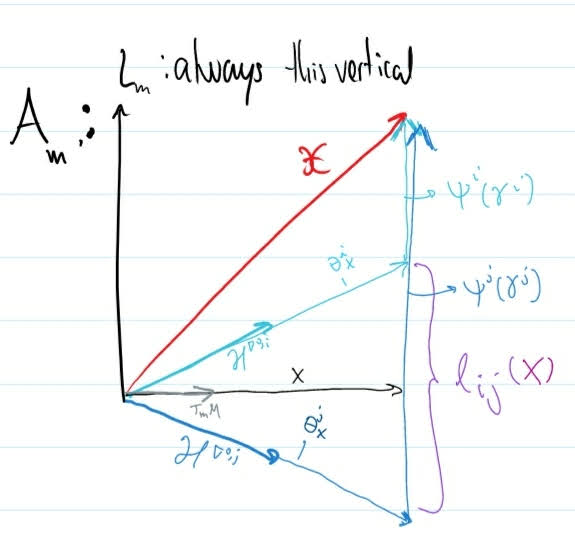
\includegraphics[width = \textwidth/2]{images/DiagramaMapasLocalesAlgebroide.jpg}
    \caption{Representation of the local maps introduced to study a transitive Lie algebroid $A$. The whole space represents, roughly, the vector space $A_m$ for $m \in M$, and $\oid X$ such that $a(\oid X) = X$ is an arbitrary element in $A_m$. Understanding $j$ as an inclusion, the vertical axis represents the adjoint Lie algebroid fiber $L_m$. The horizontal axis represents the tangent space $T_m M$, but it is not part of $A_m$, since there is no canonical horizontal direction in $A_m$. The images of $\Theta^i$ and $\Theta^j$ give two distinct notions of horizontality in $A_m$.}
    \label{fig:localMaps}
\end{figure}

\begin{theorem}
$\chi^i_j: U_{ij} \to U_{ij} \times \alg g$ is a Maurer-Cartan form, i.e. it satisfies the Maurer-Cartan equation:
\begin{align*}
    d \chi^i_j(X, Y) + [\chi^i_j(X), \chi^i_j(Y)] = 0
\end{align*} for all $X, Y \in TU_{ij}$.
\end{theorem}

\begin{proof}
Add proof is this theorem is indeed left in the document. This reduces to the fact that the standard flat connection in $U_i \times \alg g$ is mapped through $\psi^i$ to the adjoint connection $\nabla^{\Theta^i}$ in $L|_{U_i}$ induced by the flat connection $\Theta^i$ in $A|_{U_i}$. 
\end{proof}

%%%%%%%%%%%%%%%%%%%%%%%%%%%%%%%%%%%%%%%%%%%%%%%%%%%%%%%%%%%%%%%%%%%%%%%%%%%%%%%%%%%%
%%%%%%%%%%%%%%%%%%%%%%%%%%%%%%%%%%%%%%%%%%%%%%%%%%%%%%%%%%%%%%%%%%%%%%%%%%%%%%%%%%%%
\subsection{Local Description of the Atiyah Lie algebroid}

$\psi_i(\eta^i)(p) = Ad_{g^{-1}}\eta^i(x)$.

$\Theta^i(X)_p = R_{g*, s_i(x)} s_{i*, x} X_x$

If $X \oplus \eta^i$ and $X \oplus \eta^j$ are local trivializations of $\oid X$, $\sectoid X$, then

\begin{align}
    \eta^i &= g_{ij} \eta^j g_{ij}^{-1} + g_{ij} dg^{-1}_{ij}(X) \\
    \alpha^i_j(\eta) &= g_{ij} \eta  g_{ij}^{-1} \\
     \chi^i_j(X) &= g_{ij} dg_{ij}^{-1}(X) 
\end{align}

%\section{Actions of Lie Algebroids?}
%%%%%%%%%%%%%%%%%%%%%%%%%%%%%%%%%%%%%%%%%%%%%%%%%%%%%%%%%%%%%%%%%%%%%%%%%%%%%%%%%%%%
%%%%%%%%%%%%%%%%%%%%%%%%%%%%%%%%%%%%%%%%%%%%%%%%%%%%%%%%%%%%%%%%%%%%%%%%%%%%%%%%%%%%
%%%%%%%%%%%%%%%%%%%%%%%%%%%%%%%%%%%%%%%%%%%%%%%%%%%%%%%%%%%%%%%%%%%%%%%%%%%%%%%%%%%%
%%%%%%%%%%%%%%%%%%%%%%%%%%%%%%%%%%%%%%%%%%%%%%%%%%%%%%%%%%%%%%%%%%%%%%%%%%%%%%%%%%%%




%%%%%%%%%%%%%%%%%%%%%%%%%%%%%%%%%%%%%%%%%%%%%%%%%%%%%%%%%%%%%%%%%%%%%%%%%%%%%%
%%%%%%%%%%%%%%%%%%%%%%%%%%%%%%%%%%%%%%%%%%%%%%%%%%%%%%%%%%%%%%%%%%%%%%%%%%%%%%
\chapter{Differential Calculi on Lie Algebroids}\label{chp:diffStruc}
Fernandes remarks that it is thanks to the Lie braket that it is possible to make this kind of Cartan calculi.

Why is it necessary? What does this mean? What does it allow?

What is the difference, if any, with connection theory?

Relation between exterior derivative and usual covariant derivative:
    \begin{itemize}
    
    \item Finer than $d$: requiring $TM$ necessarily, because it is based on a connection $TM \to \mathcal D(E)$
    
    \item Coarser than $d$: does not require a representation, a connection doesn't have to be a homomorphism of Lie algebras.
        
    \end{itemize}

Why relevant to me:
    \begin{itemize}
        
    \item Vector calculus?
    
    \item What can be integrated. Inner integration generates usual (vector bundle valued) forms on the base manifold.
    
    \item Algebroid connections are ``normalized'' elements $ \omega \in \Omega^1(A, L)$, and their curvature is $d\omega \in \Omega^2(A, L)$. Generalized connections are precisely the elements of $\Omega^1(A, L)$.
    
    \item When talking about matter fields, a generalized connection $\hat \omega$ induces covariant derivatives $\hat \nabla^E: \Gamma(E) \to \mathbf{\Omega^1(A, E)}$, so that $\hat \nabla^E \phi \in \Omega^1(A, E)$.
    
    \item $\Omega^\bullet(A)$ is used to do cohomology on Lie algebroids
    
    \item In each $\Omega^p(A, L)$ the natural scalar product $(\omega, \eta) = \cl{\omega, \star \eta} = \int_A h(\omega, \star \eta)$, for $h$ in inner metric, is what will be used to define the gauge action:
        
        \begin{itemize}
            
        \item For $\hat \omega \in \Omega^1(A, L)$, define $S_{Gauge}[\hat \omega] = (\hat R, \hat R)$
        
        \item For $\phi \in \Gamma(E)$ and $\hat \omega$ as above, $S_{Matter}[\phi, \hat \omega] := (\hat \nabla^E \phi, \hat \nabla^E \phi)$
        
        \end{itemize}
        
    \end{itemize}

TODO\todo{check this}: the third ``important example'' introduced in Lazzarini is important to me? $A$ connections on $E$ are used to define finite gauge transformations, which somehow induce the infinitesimal gauge transformation definition on generalized connections? If not for this, $A$-connections, and so this examples, are of no relevance to me.

%%%%%%%%%%%%%%%%%%%%%%%%%%%%%%%%%%%%%%%%%%%%%%%%%%%%%%%%%%%%%%%%%%%%%%%%%%%%%%%%%%%%
%%%%%%%%%%%%%%%%%%%%%%%%%%%%%%%%%%%%%%%%%%%%%%%%%%%%%%%%%%%%%%%%%%%%%%%%%%%%%%%%%%%%
%%%%%%%%%%%%%%%%%%%%%%%%%%%%%%%%%%%%%%%%%%%%%%%%%%%%%%%%%%%%%%%%%%%%%%%%%%%%%%%%%%%%
%%%%%%%%%%%%%%%%%%%%%%%%%%%%%%%%%%%%%%%%%%%%%%%%%%%%%%%%%%%%%%%%%%%%%%%%%%%%%%%%%%%%
\section{Differential Structures and Cartan Operations}

%%%%%%%%%%%%%%%%%%%%%%%%%%%%%%%%%%%%%%%%%%%%%%%%%%%%%%%%%%%%%%%%%%%%%%%%%%%%%%%%%%%%
%%%%%%%%%%%%%%%%%%%%%%%%%%%%%%%%%%%%%%%%%%%%%%%%%%%%%%%%%%%%%%%%%%%%%%%%%%%%%%%%%%%%
\subsection{Differential Algebras}

{\color{gray}
\begin{itemize}

\item Alt

\item $\Omega$

\item $d$. Is antiderivation

\item $(\Omega, d)$ Graded differential algebras. Differential calculus (over a commutative algebra?) ?
    
    \begin{itemize}
    
    \item $(\Omega(A), \hat d_A)$ is graded commutative differential algebra
    
    \item $(\Omega(A, L), \hat d)$ is graded differential Lie algebra.
    
    \end{itemize}

\item Respect further structure... of $L$?



\end{itemize}
}

\linea 

Throughout this section, let $A$ be a Lie algebroid over the manifold $M$ with anchor $a$.

\begin{definition}
Let $E$ be a vector bundle over $M$. We now define some vector bundles over $M$.
    \begin{itemize}
    
    \item Let \emph{$\Alt^0(A, E)$}$:= E$. 
    
    \item For $n \in \ZZ_{\geq 1}$, let \emph{$\Alt^n(A, E)$} be the natural embedding, as alternating maps, of the (hom-)bundle $\Hom(\bigwedge^n A, E)$ into the vector bundle $\Hom(\bigoplus^n A, E)$ (as defined according to \ref{}) over $M$. Its fiber at $m \in M$ is, then, the vector space of alternating linear transformations $\{\omega: \underbrace{A_m \times \cdots \times A_m}_{\text{$n$ times}} \to E_m \st \text{$\omega$ is $\RR$-linear and alternating}\}$.
    
    \item Let \emph{$\Alt^\bullet(A, E)$}$:= \bigoplus^\infty_{n = 0} \Alt^n(A, E)$.
    % OJO: i can't call this forms, since forms are either C^\infty M multilinear, or complete vector bundle morphisms!
    
    %\item For $n \in \ZZ_{\geq 0}$, let \emph{$\Alt^n(A)$} and \emph{$Alt^\bullet (A)$} be the application of the previous definitions to the trivial vector bundle $E = M \times \RR$.
        
    \end{itemize}
    
\end{definition}

\begin{remark}
A local section over the open $U \subset M$ of a hom-bundle $\Hom(E, E')$, for $E$ and $E'$ vector bundles over $M$, is a vector bundle morphism $:E|_U \to E|_{U'}$ between vector bundles over $U$. Naturally, then, the elements of $\Gamma_U(\Hom(E, E'))$ are equivalent to $C^\infty(U)$-linear maps $: \Gamma_U(E) \to \Gamma_U(E)$. 

Notice, that a local section of a hom-bundle $\Hom(E, E')$ need not have an extension to a full vector bundle morphism $:E \to E'$.\todo{Even if only on $A = TS^2$, in which case we have the usual manifold theory of forms, $\partial_\phi$ is part of a local frame BUT can't be extended to a global vector field, it still defines a ``local form'' $d\phi \in \Omega_{U_{SN}}(M)$}
\end{remark}

Notice that $\Alt^\bullet(A, E)$ is indeed a vector bundle, with finite dimensional fibers, since, if $U \subset M$ is a trivializing neighborhood of both $A$ and $E$ with fibers $V$ and $W$ respectively, $\Alt^\bullet(A, E)|_U \cong U \times Hom(V, \bigwedge^* W)$ is a trivial vector bundle.

\begin{definition}
Let $E$ be a vector bundle over $M$ on which there is a representation $\phi: A \to \alg D(E)$ of $A$. Let $U \subset M$ be open:\todo{Open? Doesn't matter? I care about $U$ open only. RTA: to know what a smooth local section is, we prefer $U$ to be open}.

    \begin{itemize}
    
    \item For $n \in \ZZ_{\geq 0}$, define the $C^\infty(U)$-module \emph{\lbtext{$\Omega_U^n(A, E)$}}$:= \Gamma_U\Alt^n(A, E)$. Its elements are called \emph{local $E$-valued $n$-forms on $A$ over $U$}. If $U = M$, simply write \emph{$\Omega^n(A, E)$} and call its elements \emph{$E$-valued $n$-forms on $A$}.
    
    \item Define the $C^\infty(U)$-module $\emph{\Omega_U^\bullet(A, E)} := \bigoplus^\infty_{n = 0} \Omega_U^n(A, E)$. Its elements are simply called \emph{local $E$-valued forms on $A$ over $U$}. If $U = M$, simply write $\emph{\Omega^\bullet(A, E)}$ and call its elements \emph{$E$-valued forms on $A$.}
    
    %\item \item For $n \in \ZZ_{\geq 0}$, let \emph{$\Omega^n(A)$}$:= \Gamma\Alt^n(A)$. 
    
    %\item Define the $C^\infty(M)$-module $\emph{\Omega^\bullet(A)} := \bigoplus^\infty_{n = 0} \Omega^n(A)$.
        
    \end{itemize}
    
\end{definition}

\begin{remark}
Due to the bijective correspondence between $C^\infty(U)$-linear maps between local sections over $U$ of vector bundles and vector bundle morphisms of the bundles restricted to $U$\todo{Pretty sure this a thing. A local form need not be extendable to a global form, in the same way that the local vector field $\partial_\phi$ can not be extended to all $S^2$}, $\Omega_U^n(A, E)$ may be considered the space of $C^\infty(U)$-multilinear antisymmetric maps from $\Gamma_U(A)^n$ to $\Gamma_U(E) = \Omega_U^0(A, E)$. We will refer as \ptext{(local) $E$-valued $n$-forms on $A$} to both
\begin{align}
    \omega &: \underbrace{A|_U \oplus \cdots \oplus A|_U}_{\text{$n$ times}} \to E|_U, & \text{alternating, $\RR$-vector bundle morphism and}\\
    \omega &: \underbrace{\Gamma_U(A) \times \cdots \times \Gamma_U(A)}_{\text{$n$ times}} \to \Gamma_U(E) & \text{alternating, \dbtext{$C^\infty(U)$}-multilinear map}.
\end{align}
    
    %\item $\Omega^n(A)$ may be considered the space of $C^\infty(M)$-multilinear antisymmetric maps from $\Gamma(A)^n$ to $C^\infty(M)$.
    
\end{remark}

\lin



\begin{example}
On the trivial vector bundle $M \times \bb K$\todo{$A$ as a $\bb K$ vector bundle}, the associated space of forms on $A$ is denoted by $\lbtext{\lbtext{\Omega^\bullet(A)}}$, and it is called the \lbtext{space of scalar valued forms on $A$}. Notice that the module $\Omega^n(A) = \Gamma \bigwedge^n A^*$.

This is the fundamental example of forms on an algebroid $A$. It has been used to define a cohomology theory on Lie algebroids and \todo{complement}.
\end{example}

\begin{example}
Let $0 \to L \xrightarrow{j} A \xrightarrow{a} TM \to 0$ be a transitive Lie algebroid sequence.
The space $\lbtext{\Omega^\bullet(A, L)}$ of $L$-valued forms on $A$ will be an important example since (generalized) algebroid connections and their curvatures are particular cases of this type of forms on $A$.
\end{example}

\lin

\begin{theorem}\label{isomorphOmega}
Let $U\subset M$ be open:
    \begin{itemize}
    
    \item $\Alt^n(A, E)|_U$ and $E|_U \otimes \bigwedge^n A^*|_U$ are isomorphic vector bundles.
    
    %\item $\Alt^n(A)$ and $\bigwedge^n A^*$ are isomorphic vector bundles.
    
    \item \rtext{$\Omega_U^n(A, E)$ and $\Gamma_U(E) \otimes \Omega_U^n(A)$ are isomorphic} $C^\infty(U)$-modules.
    
    \item If $U$ is trivializing neighborhood for both $A$ and $E$, $\rtext{\Omega_U^n(A, E)} \cong C^\infty(U, V) \otimes_{C^\infty(U)} \Gamma(U \times \bigwedge^n W^*) \rtext{\cong C^\infty(U, V) \otimes_{C^\infty(M)} C^\infty\left(U, \bigwedge^n W^* \right) } \cong \rtext{ C^\infty(U, V) \otimes_{\bb K} \bigwedge^n W^*}$.
    
    %\item $\Omega^n(A)$ and $\Gamma\Alt^nA^*$ are isomorphic $C^\infty(M)$-modules.
    
    \end{itemize}
\end{theorem}

\begin{proof}
We may assume simply that $U = M$, since using an arbitrary $U$ simply means that we are working on manifolds over $U$. $\Alt^n(A, E) \cong \Hom(\bigwedge^n A, E)$ by definition, and $\Hom(\bigwedge^n A, E) \cong E \otimes (\bigwedge^n A)* \cong E \otimes \bigwedge^n A^*$, but $\bigwedge^n A^* = \Omega^n(A)$.

Since $\Gamma$ is a strong monoidal function\todo{can I make this more clear?}, it distributes over the tensor product, and so the result follows from the first part of the theorem.
\end{proof}

\linea


\ptext{In the following, assume that $E$ is a vector bundle over $M$ on which there is a representation $\phi: A \to \alg D(E)$ of the Lie algebroid $A$ over $M$}.

\begin{definition}
    \begin{itemize}
    
    \item Differential complex:
    
    \item Differential module:
        
    \end{itemize}
\end{definition}

\begin{definition}
Let $E$ be a vector bundle over $M$ on which there is a representation $\phi: A \to \alg D(E)$ of $A$. Define \emph{the differential of $E$-valued forms on $A$} by the Koszul formula:
\begin{eqnsplit*}
\lbtext{\hat d_\phi}: \Omega^{\bullet}(A, E) &\to \Omega^{\bullet+1}(A, E)
\end{eqnsplit*}
\begin{multline}
(\hat d_\phi \omega)(\sectoid X_1, \dots, \sectoid X_{p+1}) = \sum_{i=1}^{p+1} (-1)^{i+1} \phi(\sectoid X_i)\cdot \omega(\sectoid X_1, \cdots, \overset{\vee}{\sectoid X_i}, \cdots, \sectoid X_{p+1}) \\
 + \sum_{1 \leq i < j \leq p+1} (-1)^{i+j}\omega([\sectoid X_i, \sectoid X_j], \sectoid X_1, \cdots, \overset{\vee}{\sectoid X_i}, \cdots, \overset{\vee}{\sectoid X_j}, \cdots, \sectoid X_{p+1})
\end{multline}
for any $p \in \ZZ_{\geq 0}$, $p$-form $\omega$, and any $\sectoid X_1, \dots, \sectoid X_{p+1} \in \Gamma(A)$.
\end{definition}

\begin{proposition}
 $(\Omega^\bullet(A, E), \hat d_\phi)$ is a differential module. In particular, it is a differential complex.
\end{proposition}

\begin{theorem}\label{theoDifferentialLocal}
$d_U$: Leibniz w.r.t. functions giben by the previous definition.\todo{complete}. \rtext{$\hat d_\phi$ is a local operator}
\end{theorem}

\begin{remark}
So 1., 2. . \ptext{In particular, \textbf{all of the remaining results of this section are still valid when applied to local forms, replacing every instance of $\Omega$ by $\Omega_U$.}}
\end{remark}

\lin

\begin{definition}\label{defnDiffGModule}
    Let $M = \oplus_{n = 0}^\infty M^n$ graded module over the graded ring $R = \oplus_{n = 0}^\infty R^n$, i.e. an $R$-module such that $R^p \cdot M^q \subset M^{p+q}$.
    
    \begin{itemize}
    
    \item An element $\omega \in N^n$ is called a \emph{homogeneous element of degree $n$}, for $n \in \ZZ_{\geq 0}$, and its degree is denoted by $|\omega|$.
    
    \item An \emph{antiderivation on $M$} is an $R$-linear map $d: M \to M$ such that, if $\omega$ is homogeneous, 
    \begin{align*}
        d(\omega \, \eta) = (d\omega)\tau + (-1)^{|\omega|} \omega (d\tau)
    \end{align*}
    
    \item An antiderivation $d: M \to M$ is \emph{of degree $m \in \ZZ$} if, for all homogeneous elements $\omega \in M$,
    \begin{align*}
        |d\omega| = |\omega| + m.
    \end{align*}
    If the antiderivation is of degree $1$ or $-1$, it is called a \emph{differential on $M$}.
    
    \item Let $M = \oplus_{n = 0}^\infty M^n$ be a graded module and $d: M \to M$ a differential on $M$. $(M, d)$ is called a \emph{differential graded module over $R$} if $d \circ d = 0$.
    
    \item Let $(M, d)$ and $(M', d')$ be differential graded modules over $R$. A \emph{morphism of differential graded modules} is a graded module morphism $\phi: M \to M'$, i.e. an $R$-linear map that sends homogeneous elements of degree $m \in \ZZ$ of $M$ into similar elements in $M'$, such that $d' \circ \phi = \phi \circ d$.
    
    \end{itemize}
    
\end{definition}

\begin{definition}
Define the $C^\infty(M)$-bilinear operation operation
\begin{align*}
    \lbtext{\wedge}: \Omega^\bullet(A) \times \Omega^\bullet(A, E) &\to \Omega^\bullet(A, E)
\end{align*}
for any $p, q \in \ZZ_{\geq 0}$,
through the linear extension on the homogeneous elements:
\begin{eqnsplit}
(\omega \wedge \eta)(\sectoid X_1, \dots, \sectoid X_{p+q}) &:= \\
\frac{1}{p!q!} \sum_{\sigma \in S_{p+q}} &(-1)^{\sigma} 
\underbrace{\omega(\oid X_{\sigma(1)}, \cdots, \oid X_{\sigma(p)})}_{\in \,\Gamma(M \times \RR)} 
\cdot 
\underbrace{\eta(\oid X_{\sigma(p+1)}, \cdots, \oid X_{\sigma(p+q)})}_{\in \, \Gamma(L)}
\end{eqnsplit}
for any real valued $p$-form $\omega$, $L$-valued $q$-form $\eta$ and any $\sectoid X_1, \dots, \sectoid X_{p+q} \in \Gamma(A)$.
\end{definition}

\ptext{When the $E$-valued form is a $0$-form, i.e. a section of $\Gamma(E)$, the $\wedge$ symbol is usually not written}.

\begin{theorem}\label{theoFormsAreDiffGModule}
 \rtext{$(\Omega^\bullet(A, E), \hat d_\phi)$ is a graded differential module over $\Omega^\bullet(A)$}.
\end{theorem}

\begin{proof}
To see:

$\Omega^p(A) \wedge \Omega^q(A, E) \subset \Omega^{p+q}(A, E)$.
\end{proof}

\begin{example}
Let $A$ act by the trivial action $\phi^0: A \to \alg D(M \times \bb K)$, i.e. considering $\Gamma(M \times \RR)$ as $C^\infty(M)$ and letting the representation be the anchor. The associated differential on $\Omega^\bullet(A)$ will be denoted by $\hat d_A$, making of \lbtext{$(\Omega^\bullet(A), \hat d_A)$} a differential graded module
\end{example}

\begin{example}
Let $0 \to L \xrightarrow{j} A \xrightarrow{a} TM \to 0$ be a transitive Lie algebroid sequence.
The differential graded module associated to the adjoint action defined in \ref{defnAdjointAct}, $ad: A \to \alg D(L)$, $\oid X \mapsto j^{-1}[\oid X, \cdot]$, will be denoted by \lbtext{$(\Omega^\bullet(A, L), \hat d)$}.
\end{example}

\lin

\begin{definition} \label{defnDiffGAlgebra}
Let $\mathcal A = \oplus_{n = 0}^\infty \mathcal A^n$ be a graded algebra (over the field $\bb K$), and let $\cdot$ denote the product.
    \begin{itemize}
    
    \item An element $\omega \in \mathcal A^n$ is called a \emph{homogeneous element of degree $n$}, for $n \in \ZZ_{\geq 0}$, and its degree is denoted by $|\omega|$.
    
    \item An \emph{antiderivation on $\mathcal A$} is an $\bb K$-linear map $d: \mathcal A \to \mathcal A$ such that, if $\omega$ is homogeneous, 
    \begin{align*}
        d(\omega \bullet \eta) = (d\omega)\bullet\tau + (-1)^{|\omega|} \omega \bullet (d\tau)
    \end{align*}
    
    \item An antiderivation $d: \mathcal A \to \mathcal A$ is \emph{of degree $m \in \ZZ$} if, for all homogeneous elements $\omega \in \mathcal A$,
    \begin{align*}
        |d\omega| = |\omega| + m.
    \end{align*}
    If the antiderivation is of degree $1$ or $-1$, it is called a \emph{differential on $\mathcal A$}.
    
    \item Let $d: \mathcal A \to \mathcal A$ be a differential on $A$. Then the pair $(A, d)$ is called a \emph{differential graded algebra} if $d \circ d = 0$. 
    
    \item Let $(\mathcal A, \bullet, d)$ and $(\mathcal A', \bullet', d')$ be differential graded algebras. A \emph{morphism of differential graded algebras} is a graded algebra morphism $\phi: \mathcal A \to \mathcal A'$ such that $d' \circ \phi = \phi \circ d$.
    
    \end{itemize}
    
\end{definition}


\begin{definition}
Let $E$ be an algebra bundle over $M$ with fiberwise multiplication $\bullet$, i.e. a vector bundle such that each fiber is an algebra and such that there exists an atlas compatible with the algebra multiplication, on which $A$ is represented. Define on $\Omega^\bullet(A, E)$ the $C^\infty(M)$-bilinear operation operation, called \emph{the wedge product of LAB-valued forms on $A$}
\begin{eqnsplit*}
\wedge^\bullet : \Omega^\bullet(A, E) &\times \Omega^\bullet(A, E) \to \Omega\bullet(A, E)
\end{eqnsplit*}
as the linear extension of the maps, for any $p, q \in \ZZ_{\geq 0}$
\begin{eqnsplit*}
\wedge^\bullet : \Omega^p(A, E) \times \Omega^q(A, E) &\to \Omega^{p+q}(A, E)
\end{eqnsplit*}
\begin{eqnsplit}
(\omega \wedge \eta)(\sectoid X_1, \dots, \sectoid X_{p+q}) &:= \\
\frac{1}{p!q!} \sum_{\sigma \in S_{p+q}} &(-1)^{\sigma} \omega(\oid X_{\sigma(1)}, \cdots, \oid X_{\sigma(p)}) \bullet \eta(\oid X_{\sigma(p+1)}, \cdots, \oid X_{\sigma(p+q)}).
\end{eqnsplit}
for any $p$-form $\omega$, $q$-form $\eta$ and any $\sectoid X_1, \dots, \sectoid X_{p+q} \in \Gamma(A)$.%, where $\bullet$ is the algebra multiplication induced on $\Gamma(E)$ by the fiberwise algebra multiplication in $E$.
\end{definition}

\begin{theorem} \label{theoFormsAreDiffGAlgebebra}
Let $E$ be an algebra bundle over $M$ on which there is a representation $\phi: A \to \alg D(E)$ of $A$. \rtext{Then $(\Omega^\bullet(A, E), \wedge^\bullet, \hat d_\phi)$ is a differential graded algebra over $\Omega^\bullet(A)$}.
\end{theorem}

\begin{proof}
To see:

Graded Leibniz
\end{proof}


\begin{example}
Since $\Omega^\bullet(A)$ is simply an abreviation for $\Omega^\bullet(A, M \times \bb K)$, \rtext{$(\Omega^\bullet(A), \wedge, \hat d_A)$ is a graded-commutative differential graded algebra} over $\Omega^\bullet(A)$, where $\wedge = \wedge^\cdot$, for $\cdot$ the multiplication in $\bb K$.

The additional conditions is simply that $\alpha \beta = (-1)^{|x||y|}\beta \alpha$ for all homogeneous elements $\alpha, \beta$. This follows from $\bb K$ being commutative.
\end{example}

\begin{example}
$(\Omega^\bullet(A, L, \wedge^{[,]}, \hat d)$ is a Lie-graded differential graded algebra.\todo{Useful? Perhaps when defining curvatures via something similar to structure equation?... Rta: it should be possible to use when defining the Atiyah Lie algebroid connection, and so in all transitive Lie algbroids, but we don't do it, we instead use the shorthand $[,]$ notation, which isn't the $[,] \equiv \wedge^{[,]}$}

\end{example}

\linea

The following important theorem relates the notions of vector valued connections on principal bundles, that give rise to principal connections and their curvatures, and the theory of forms on the Atiyah Lie algebroid associated to the principal bundle.

\begin{theorem}\label{theoFormsPpalAtiyahSame}
Let $G \to P \to M$ be a principal bundle over $M$. 
\begin{itemize}
    \item The differential graded module and algebra \rtext{$(\Omega^\bullet(TP/G), \hat d_{TS^3/S^1})$ is isomorphic to the subspace of $(\Omega^\bullet(TP), d)$ associated to the $R_*$-invariant  forms on $P$}.
    
    \item Similarly, the differential graded module and algebra \rtext{$(\Omega^\bullet(TP/G, P \times \alg g/G), \hat d)$ is isomorphic to the subspace of $(\Omega^\bullet(TP) \otimes \alg g, d)$ associated to the $(R_*, Ad)$-equivariant $\alg g$-valued forms on $P$}.
\end{itemize} 
\end{theorem}

\linea

\begin{example}
Let $A = TM$ given a manifold $M$. Then $(\Omega^\bullet (TM), \wedge, \hat d_{TM})$ is precisely the usual differential graded algebra and module $(\Omega^\bullet (M), \wedge, d)$ of forms on $M$.

Letting $E = M \times V$ given a vector space $V$, on which $TM$ is represented trivially by $i: TM \to \alg D(E)$, $X \mapsto X$, the differential graded module $(\Omega^\bullet(TM, M \times V), \hat d_i)$ is precisely the traditional $(\Omega^\bullet(M, V), d)$. If $V$ is an algebra with operator $\bullet$, for example a Lie algebra $\alg g$ with operation $[\cdot, \cdot]$, $(\Omega^\bullet(TM, E), \wedge^\bullet, \hat d_i)$ is exactly the traditional differential graded algebra $(\Omega^\bullet(M, V), \bullet, d)$.
\end{example}

\begin{example}
Let $E$ be a vector bundle over $M$, and suppose that on the open $U \subset M$, $\{\sect \mu_1, \dots, \sect \mu_d\} \subset \Gamma_U(E)$ and $\{\sectoid X^1, \dots, \sectoid X^N\} \subset \Gamma_U(A)$ and  are local frames
\todo{\rtext{WAIT!} Even if only on $A = TS^2$, in which case we have the usual manifold theory of forms, $\partial_\phi$ is part of a local frame BUT can't be extended to a global vector field, it still defines a local form $d\phi \in \Omega_{U_{SN}}(M)$}
. For this local frame of $A$, let the dual frame be $\{\alpha_1, \dots \alpha_N\} \in \Gamma_U(A^*)$, hence satisfying $\alpha_i(\sectoid X^j) = \delta_{ij} \in C^\infty(U)$. Then:

    \begin{itemize}
        
    \item Each $\alpha_i$, $i = 1, \dots, N$, is in fact a local $1$-form in $\Omega_U^1(A) = \Gamma_U(A^*)$.
    
    \item $\alpha_{i_1} \wedge \alpha_{i_p}$ is an element of $\Omega_U^p(A)$.
    
    \item For any $f \in C^\infty(U)$, 
    \begin{equation}
        f\, \alpha_{i_1} \wedge \cdots \wedge \alpha_{i_p},
    \end{equation} 
    $i_1, \dots, i_p = 1, \dots, N$, is also an element of $\Omega_U^p(A)$. In fact, any scalar valued $p$-form on $A$ is a linear combination of forms of this type.\todo{Is this true? }
    
    \item For any $\mu \in \Gamma_U(E) = \Omega_U^0(A, E)$, 
    \begin{equation}
        \mu \wedge \alpha_{i_1} \wedge \cdots \wedge \alpha_{i_p},
    \end{equation}
    $i_1, \dots, i_p = 1, \dots, N$, is an element of $\Omega_U^p(A, E)$, where the first $\wedge$ refers to the product between the scalar valued $p$-form $\alpha_{i_1} \wedge \cdots \wedge \alpha_{i_p}$ and the $L$-valued $0$-form $\mu$. In fact, any scalar valued $p$-form on $A$ is a linear combination of forms of this type.
        
    \end{itemize}
\end{example}


\begin{example}[Hopf $S^3$]
Recall that $\{\underline{\partial_\phi}, \underline{\partial_{\xi^1}}, \underline{\partial_{\xi^2}}\}$ is a local frame of the Atiyah Lie algebroid associated to the complex Hopf principal bundle $S^1 \to S^3 \to S^2$. 

So, the building blocks of any local form over $U_{SN}$ will be the dual frame, which we will denote by $\{\underline{d\phi}, \underline{d\xi_1}, \underline{\xi_2}\} \in \Omega^1(TS^3/S^1)$. 

Since $L = S^3 \times i\RR / S^1$ has the global frame $\{i\}$, \rtext{any section of $L$ can be written as $f\,i$ for some $f \in C^\infty(S^2)$}. Hence, \rtext{any $S^3 \times i\RR/S^1$-valued local form on $TS^3/S^1$ can be written as a multiplication via wedge product of the forms $\{\underline{d\phi}, \underline{d\xi_1}, \underline{\xi_2}\}$, with coefficients in $C^\infty(S^2, i\RR)$}.

An important local $1$-form on $TS^3/S^1$ over $U_{SN}$ is
\begin{equation}
    \lbtext{\omega^{Monop}_{U_{SN}}} := \frac{i}{2} d\xi^1 (1 + \cos \phi) \underline{d \xi_1} + \frac{i}{2} (1- \cos\phi)\underline{d\xi_2} \in \Omega_{U_{SN}}^1(TS^3/S^1, S^3 \times i\RR/S^1).
\end{equation} This $1$-form is associated to the presence of a magnetic monopole on $3$-dimensional space.

Due to theorem \ref{theoFormsPpalAtiyahSame}, the differential $d$ of $G$-invariant forms on $P$ corresponds to the differential $\hat d_{TS^3/S^1}$ under the identification of $G$-invariant sections of $TS^3$ with sections of $TS^3/S^1$ denoted by an underline. Hence, $\hat d_{TS^3/S^1} \underline{\xi_i} = \underline{d \xi_i}$, and, since $d^2 = 0$, 
\begin{equation*}
    \hat d_{TS^3/S^1} {\underline{d\xi_i}} = 0
\end{equation*} for $i = 1, 2$; similarly 
\begin{equation*}
     \hat d_{TS^3/S^1} \underline{d \phi} = 0.
\end{equation*}

Now, applying the graded Leibniz rule to the above $1$-form considerint it a sum of products of $S^3\times i\RR/S^1$-valued $0$-forms and scalar valued $1$-forms, we conclude that
\begin{equation}
    \lbtext{R^{MP}_{U_{SN}}} 
    := \hat d \omega^{Monop}_{U_{SN}} = -\frac{i}{4} \sin \phi \, \underline{d\phi} \wedge (\underline{d\xi_1} - \underline{d\xi_2}) 
    \in \Omega^2(TS^3/S^1, S^3 \times i\RR / S^1).
\end{equation}
\end{example}


%%%%%%%%%%%%%%%%%%%%%%%%%%%%%%%%%%%%%%%%%%%%%%%%%%%%%%%%%%%%%%%%%%%%%%%%%%%%%%%%%%%%
%%%%%%%%%%%%%%%%%%%%%%%%%%%%%%%%%%%%%%%%%%%%%%%%%%%%%%%%%%%%%%%%%%%%%%%%%%%%%%%%%%%%
{\color{gray} This only seems to be useful if we want to define the alternative description of the Atiyah Lie algebroid found in Lazzarini2012

\subsection{Cartan Operations}

% \begin{itemize}

% \item $i, L$

% \item Horizontal, invariant and basic forms.

% \end{itemize}

\begin{definition}
Let $E$ be an algebra bundle over $M$, let $\phi: A \to \alg D(E)$ be a representation of $A$, and let $B$ be a Lie algebroid over $M$. A \emph{Cartan operation on $(\Omega^\bullet(A, E), \wedge, \hat d_\phi)$} is a triple $(B, i, L)$ such that: for any $\sectoid X \in B$, for any $p \geq 1$ there is a map $i_{\sectoid X}: \Omega^p(A, E) \to \Omega^{p-1}(A, E)$ such that, defining 
\begin{align}
L_{\sectoid X} := \hat d_\phi i_{\sectoid X} + i_{\sectoid X}\hat d_\phi,
\end{align}
the following relations hold for any $\sectoid X, \sectoid Y \in B$ and $f \in C^\infty(M)$:
\begin{align}
    i_{f \sectoid X} = f i_{\sectoid X} & i_{\sectoid X} i_{\sectoid Y} + i_{\sectoid Y} i_{\sectoid X} = 0 \\
    [L_{\sectoid X}, i_{\sectoid Y}] = i_{[\sectoid X, \sectoid Y]} & [L_{\sectoid X}, L_{\sectoid Y}] = L_{[\sectoid X, \sectoid Y]}
\end{align}
\end{definition}

\begin{example}
$B = A$ defines one.
\end{example}

\begin{example}
$B = L$ also defines one.
\end{example}

\begin{definition}
Let $(B, i, L)$ be a Cartan operation on $(\Omega^\bullet(A, E), \wedge, \hat d_\phi)$.
    
    \begin{itemize}
        
    \item Define $\Omega^\bullet(A, E)_{Hor}$ to be the graded subspace of \emph{horizontal elements in $\Omega^\bullet(A, E)$} characterized by 
    \[
    i_{\sectoid X} \omega = 0?
    \]
    
    \item Define $\Omega^\bullet(A, E)_{Inv}$ to be the graded subspace of \emph{invariant elements in $\Omega^\bullet(A, E)$} characterized by 
    \[
    L_{\sectoid X} \omega = \omega?
    \]
    
    \item Define $\Omega^\bullet(A, E)_{Basic} = \Omega^\bullet(A, E)_{Hor} \inter \Omega^\bullet(A, E)_{Inv}$ to be the graded subspace of \emph{basic or tensorial elements in $\Omega^\bullet(A, E)$}.
        
    \end{itemize}
    
\end{definition}

\begin{example}
Atiyah. The concept coincides? (See Mackenzie)
\end{example}}
%%%%%%%%%%%%%%%%%%%%%%%%%%%%%%%%%%%%%%%%%%%%%%%%%%%%%%%%%%%%%%%%%%%%%%%%%%%%%%%%%%%%
%%%%%%%%%%%%%%%%%%%%%%%%%%%%%%%%%%%%%%%%%%%%%%%%%%%%%%%%%%%%%%%%%%%%%%%%%%%%%%%%%%%%
%%%%%%%%%%%%%%%%%%%%%%%%%%%%%%%%%%%%%%%%%%%%%%%%%%%%%%%%%%%%%%%%%%%%%%%%%%%%%%%%%%%%
%%%%%%%%%%%%%%%%%%%%%%%%%%%%%%%%%%%%%%%%%%%%%%%%%%%%%%%%%%%%%%%%%%%%%%%%%%%%%%%%%%%%
\section{Trivial Lie Algebroid}

{\color{gray}
\begin{itemize}
    
\item $(\Omega(A), \hat d_A)$ as $(\Omega(M)\otimes \bigwedge g^*, d + s =: \lbtext{\hat d_{triv}})$.

\item $(\Omega(A, L), \hat d)$ as $(\Omega(M)\otimes \bigwedge g^* \otimes \mathfrak g, d + s')$ : \[(\Omega_{TLA}(M, \mathfrak g), \lbtext{\hat d_{TLA} =: \hat d})\]

\item Generic element in $\Omega^n$, given dual basis $\theta = \set{\theta^a}$ of a basis of $\alg g$ $\set{E_a}$
\begin{align*}
    \omega = \sum_{p + s = n} \omega^\theta_{\mu_1 \cdots a_1 \cdots a_s} dx^{\mu_1} \wedge \cdots \theta^{a_s}
\end{align*}
    
\end{itemize}
}
\linea

Let $A = TM \oplus (M \times \alg g)$ be a trivial Lie algebroid over the manifold $M$, with $\alg g$ a Lie algebra.

\begin{proposition}\label{propIsoScalarFormsTLA}
The $C^\infty(M)$-module of $\bb K$-valued forms on the trivial Lie algebroid bundle $TM \times \alg g$ is isomorphic\todo{even equal} to $\Omega^\bullet(TM) \otimes_{\bb K} \bigwedge^\bullet \alg g^* = \Omega^\bullet(TM) \otimes_{C^\infty(M)} C^\infty(M, \bigwedge^\bullet \alg g^*)$. The isomorphism, defined by linear extension of
\begin{align*}
    \Omega^r(TM) \otimes C^\infty(U, \bigwedge^s \alg g^*) &\to \Omega^{r+s}(TM \times \alg g)\\
    \alpha \otimes \beta &\mapsto \tilde \alpha \wedge \tilde \beta
\end{align*} where, for any $\alpha \in \Omega^r(TM)$ $r, s \in \ZZ_{\geq 0}$:
\begin{align*}
    \tilde \alpha: (\Gamma(TM) \times C^\infty(M, \alg g)) \times \cdots (\Gamma(TM) \times C^\infty(M, \alg g)) &\to C^\infty(M) \\
    (X_1 \oplus \tilde \eta_1, \dots, X_r \oplus \tilde \eta_r) &\mapsto \alpha(X_1, \dots, X_r)
\end{align*} and for any $\beta \in C^\infty(M, \bigwedge^s \alg g^*)$:
\begin{align*}
    \tilde \beta: (\Gamma(TM) \times C^\infty(M, \alg g)) \times \cdots (\Gamma(TM) \times C^\infty(M, \alg g)) &\to C^\infty(M) \\
    (X_1 \oplus \tilde \eta_1, \dots, X_s \oplus \tilde \eta_s) &\mapsto \beta(\tilde \eta_1, \dots, \tilde \eta_s)
\end{align*}
is compatible with the grading, where the set of homogeneous elements of degree $p \in \ZZ_{\geq 0}$ are $\sum_{r + s = p} \Omega^r(TU) \otimes_{C^\infty(M)} C^\infty(M, \bigwedge^s \alg g^*)$.
\end{proposition}

\begin{remark}
The previous isomorphism between $\Omega^\bullet(TM \times \alg g)$ and $\Omega^\bullet(TM) \otimes_{\bb K} \bigwedge^\bullet \alg g^*$ can, and will, be used to define a $C^\infty(M)$-linear multiplication $\lbtext{\wedge}$ on $\Omega^\bullet(TM) \otimes_{\bb K} \bigwedge^\bullet \alg g^*$ which is compatible with the gradings. 

Furthermore, this isomorphisms allows us to see $\Omega^\bullet(TM)$ and $C^\infty(M, \alg g)$ as subsets of $\Omega^\bullet(TM \times \alg g)$, in which case the $\Omega^\bullet(TM)$-multiplication on the latter differential graded module coincides with the wedge product within $\Omega^\bullet(TM \times \alg g)$. Abusing notation we may ignore the $~$'s of the mapping to simply state that, for $\alpha \in \Omega^r(TM)$ and $\beta \in C^\infty(M)\otimes_{\bb K} \bigwedge^s \alg g^*$, $r, s \in \ZZ_{\geq 0}$, \ptext{$\alpha \wedge \beta \in \Omega^{r+s}(TM \times \alg g)$}. 
\end{remark}

\begin{definition}
Let
\begin{align}
    d: \Omega^\bullet(TM) \otimes \bigwedge^\bullet \alg g^* &\to \Omega^{\bullet+1}(TM) \otimes \bigwedge^\bullet \alg g^*\\
    \alpha \otimes 1 &\mapsto d\alpha \otimes 1
\end{align}
be the usual de Rham differential on $\Omega^\bullet(TM)$ applied to the first factor, and
\begin{align*}
    s: \Omega^\bullet(TM) \otimes \bigwedge^\bullet \alg g^* &\to \Omega^\bullet(TM) \otimes \bigwedge^{\bullet+1} \alg g^* \\
    1 \otimes \beta &\mapsto 1 \otimes s\beta, 
\end{align*} where, given $\eta_i \in C^\infty(M, \alg g)$,
\begin{multline}
    s\beta(\sect \eta_1, \cdots, \sect \eta_{p+1}) := \sum_{1 \leq i < j \leq p+1} (-1)^{i+j} \beta([\sect \eta_i, \sect \eta_j], \sect \eta_1, \cdots, \overset{\vee}{\sect \eta_i}, \cdots, \overset{\vee}{\sect \eta_j}, \cdots \sect \eta_{p+1})
\end{multline}
be \emph{the Chevalley-Eilenbert differential on $\bigwedge \alg g^*$}, applied to the second factor. On $\Omega^\bullet(TM) \otimes \bigwedge^\bullet \alg g^*$ define the $C^\infty(M)$-linear endomorphism $\lbtext{\hat d_{triv}}$:
\begin{align}
    \hat d_{triv}: \Omega^r(TM) \otimes \bigwedge^s \alg g^* &\to \left( \Omega^\bullet(TM) \otimes \bigwedge^\bullet \alg g^*\right)^{r+s+1} \\
    \alpha \otimes \beta = \alpha \wedge \beta &\mapsto  \hat d_{triv} (\alpha \wedge \beta) := d\alpha \wedge \beta + (-1)^|\alpha| \alpha \wedge s\beta \\
    \alpha \otimes 1 &\mapsto \hat d_{triv}\alpha = d\alpha \in \Omega^{r+1}(TM) \otimes 1 \\
    1 \otimes \beta &\mapsto \hat d_{triv}\beta = s\beta \in 1 \otimes \bigwedge^{s+1} \alg g^*.
\end{align} $\hat d_{triv}$ is sometimes also denoted by $d+s$ in the literature.

\end{definition}

\begin{theorem}\label{theoIsoScalarFormsTLA}
\rtext{$(\Omega^\bullet(TM) \otimes \bigwedge^\bullet, \wedge, \hat d_{triv})$ is a (bi)graded (commutative) differential algebra and a graded differential module over $\Omega^\bullet(TM \times \alg g)$, isomorphic to the space $(\Omega^\bullet(TM \times \alg g), \wedge, \hat d_{TM \times \alg g})$} of $\bb K$-valued forms on the trivial Lie algebroid $TM \times \alg g$.
\end{theorem}

\begin{proof}
To see:

Graded module: done already, pretty much by definition of wedge, when restricting to the ``subspace'' $\Omega^\bullet(TM)$ in the first entry.

$\hat d_{triv}$ is a differential of module and algebra: pretty much by definition

Is isomorphism of graded modules: Respects the differentials DO!\todo{Done in my handwritten notes.}

Is isomorphism of graded algebras: Respects the wedge product: by definition of the wedge on the new space as defined in the remark following theorem \ref{propIsoScalarFormsTLA}.
\end{proof}

\ptext{Due to this isomorphism, from now on we will call $(\Omega^\bullet(TM) \otimes \bigwedge^\bullet \alg g^*, \wedge, \hat d_{triv})$ the space of scalar valued forms on the trivial Lie algebroid $TM \times \alg g$, and $\Omega^\bullet(TM)$ and $C^\infty(M, \bigwedge^\bullet \alg g*)$ as subspaces.}

\linea

We now apply a similar result to the $L$-valued forms on the trivial Lie algebroid $A = TM \times \alg g$.

\begin{theorem}
The $C^\infty(M)$-module $\Omega(TM \times \alg g, M \times \alg g)$ of $M \times \alg g$-valued forms on the trivial Lie algebroid bundle $TM \times \alg g$, is isomorphic to $\Omega^\bullet(TM) \otimes \left(\bigwedge^\bullet \alg g^* \otimes \alg g\right)$, and this isomorphism is compatible with the grading, where the set of homogeneous elements of degree $p \in \ZZ_{\geq 0}$ is $\left( \Omega^\bullet(TM) \otimes \left(\bigwedge^\bullet \alg g^* \otimes \alg g\right) \right)^p = \sum_{r + s = p} \Omega^r(TM) \otimes \left(\bigwedge^s \alg g^* \otimes \alg g\right)$. 

\todo{not clear where it comes from, perhaps after $d$}This isomorphism induces a $C^\infty(M)$-multilinear mapping
\begin{equation}
    \wedge: \Omega^\bullet(TM) \times \Omega^\bullet(TM) \otimes \left(\bigwedge^s \alg g^* \otimes \alg g\right)
    \to 
    \Omega^\bullet(TM) \otimes \left(\bigwedge^s \alg g^* \otimes \alg g\right).
\end{equation}

Furthermore, defining the $C^\infty(M)$-linear endomorphism $\hat d$ on this space, 
\begin{align}
    \hat d: \Omega^r(TM) \otimes \left(\bigwedge^s \alg g^* \otimes \alg g\right) &\to \left( \Omega^\bullet(TM) \otimes \left(\bigwedge^\bullet \alg g^* \otimes \alg g\right)\right)^{r+s+1} \\
    \alpha \otimes \beta = \alpha \wedge \beta &\mapsto  \hat d (\alpha \wedge \beta) := d\alpha \wedge \beta + (-1)^|\alpha| \alpha \wedge s'\beta \\
    \alpha \otimes 1 &\mapsto \hat d\alpha = d\alpha \in \Omega^{r+1}(TM) \otimes 1 \\
    1 \otimes \beta &\mapsto \hat d\beta = s'\beta \in 1 \otimes \bigwedge^{s+1} \alg g^*.
\end{align}
where $d$ is the deRhan cohomology differential applied to the first factor, and, similarly, $s'$ is the \emph{the Chevalley-Eilenbert differential on the $\alg g$-valued forms $\bigwedge \alg g^* \otimes \alg g$} applied to the second factor. This last mapping satisfies
\begin{align*}
    s': \Omega^\bullet(TM) \otimes \left(\bigwedge^\bullet \alg g^* \otimes \alg g\right) &\to \Omega^\bullet(TM) \otimes \left(\bigwedge^{\bullet+1} \alg g^* \otimes \alg g\right),
\end{align*} when applied to functions $\eta_i \in C^\infty(M, \alg g)$, gives the $\alg g$-valued function
\begin{multline}
    s'\omega(\sect \eta_1, \cdots, \sect \eta_{p+1}) := \sum_{i = 0}^{p+1} (-1)^i [\sect \eta_i, \omega(\sect \eta_1, \cdots, \overset{\vee}{\sect \eta_i}, \cdots, \sect \eta_{p+1})] \\
    \sum_{1 \leq i < j \leq p+1} (-1)^{i+j} \omega([\sect \eta_i, \sect \eta_j], \sect \eta_1, \cdots, \overset{\vee}{\sect \eta_i}, \cdots, \overset{\vee}{\sect \eta_j}, \cdots \sect \eta_{p+1}).
\end{multline}

Finally, \rtext{$\left( \Omega^\bullet(TM) \otimes \left(\bigwedge^\bullet \alg g^* \otimes \alg g\right), \hat d \right)$ is a graded differential module over $\Omega^\bullet(M)$ under the $\wedge$ product, isomorphic to $(\Omega^\bullet(TM \times \alg g, M \times \alg g), \hat d)$}.
\end{theorem}

\ptext{Due to this isomorphism, from now on we will call $(\Omega^\bullet(TM) \otimes \left(\bigwedge^\bullet \alg g^* \otimes \alg g\right), \hat d)$ the space of $\alg g$-valued forms on the trivial Lie algebroid $TM \times \alg g$, and $\Omega^\bullet(TM)$, $\Omega^\bullet(TM)\otimes \alg g$, $C^\infty(M, \bigwedge^\bullet \alg g*)$ and $C^\infty(M, \bigwedge^\bullet \alg g*)\otimes \alg g$ as subspaces.}

\begin{proof}
To see:

See proofs of the previous 2 results.

\end{proof}


\linea

{\color{gray}(Copy paste of $L$-valued)}\todo{needed for Matter action}

Let $E = M \times V$ be a trivial vector bundle over $M$ with the vector space $V$ as the fiber, and let $A = TM \times \alg g$ be represented on $E$ through $\phi: TM \times \alg g \to \alg D(M \times V)$. For example, if $V$ is a representation space of $G$, $V$ is also a representation space for $\alg g$, and this induces naturally a representation $\phi$.

\begin{theorem}
The $C^\infty(M)$-module $\Omega(TM \times \alg g, M \times V)$ of $M \times V$-valued forms on the trivial Lie algebroid bundle $TM \times \alg g$, is isomorphic to $\Omega^\bullet(TM) \otimes \left(\bigwedge^\bullet \alg g^* \otimes V\right)$, and this isomorphism is compatible with the grading, where the set of homogeneous elements of degree $p \in \ZZ_{\geq 0}$ is $\left( \Omega^\bullet(TM) \otimes \left(\bigwedge^\bullet \alg g^* \otimes V\right) \right)^p = \sum_{r + s = p} \Omega^r(TM) \otimes \left(\bigwedge^s \alg g^* \otimes V\right)$. 

This isomorphism induces a $C^\infty(M)$-multilinear mapping
\begin{equation}
    \wedge: \Omega^\bullet(TM) \times \Omega^\bullet(TM) \otimes \left(\bigwedge^s \alg g^* \otimes V\right)
    \to 
    \Omega^\bullet(TM) \otimes \left(\bigwedge^s \alg g^* \otimes V\right).
\end{equation}

Furthermore, defining the $C^\infty(M)$-linear endomorphism $\hat d$ on this space, 
\begin{align}
    \hat d_\phi: \Omega^r(TM) \otimes \left(\bigwedge^s \alg g^* \otimes V\right) &\to \left( \Omega^\bullet(TM) \otimes \left(\bigwedge^\bullet \alg g^* \otimes V\right)\right)^{r+s+1} \\
    \alpha \otimes \beta = \alpha \wedge \beta &\mapsto  \hat d_\phi (\alpha \wedge \beta) := d\alpha \wedge \beta + (-1)^{|\alpha|} \alpha \wedge \hat d_{\phi} \beta \\
    \alpha \otimes 1 &\mapsto \hat d\alpha = d\alpha \in \Omega^{r+1}(TM) \otimes 1 
\end{align}
where $d$ is the deRhan cohomology differential applied to the first factor, and, similarly, $\hat d_\phi$ applied to the second factor is defined by
\begin{align*}
    \hat d_\phi: \Omega^\bullet(TM) \otimes \left(\bigwedge^\bullet \alg g^* \otimes V\right) &\to \Omega^\bullet(TM) \otimes \left(\bigwedge^{\bullet+1} \alg g^* \otimes V\right),
\end{align*} when applied to functions $\eta_i \in C^\infty(M, V)$, gives the $V$-valued function
\begin{multline}
    \hat d_\phi\omega(\sect \eta_1, \cdots, \sect \eta_{p+1}) := \sum_{i = 0}^{p+1} (-1)^i \phi(\sect \eta_i) \cdot \omega(\sect \eta_1, \cdots, \overset{\vee}{\sect \eta_i}, \cdots, \sect \eta_{p+1}) \\
    \sum_{1 \leq i < j \leq p+1} (-1)^{i+j} \omega([\sect \eta_i, \sect \eta_j], \sect \eta_1, \cdots, \overset{\vee}{\sect \eta_i}, \cdots, \overset{\vee}{\sect \eta_j}, \cdots \sect \eta_{p+1}).
\end{multline}

Finally, \rtext{$\left( \Omega^\bullet(TM) \otimes \left(\bigwedge^\bullet \alg g^* \otimes V\right), \hat d_\phi \right)$ is a graded differential module over $\Omega^\bullet(M)$ under the $\wedge$ product, isomorphic to $(\Omega^\bullet(TM \times \alg g, M \times V), \hat d_\phi)$}.
\end{theorem}


%%%%%%%%%%%%%%%%%%%%%%%%%%%%%%%%%%%%%%%%%%%%%%%%%%%%%%%%%%%%%%%%%%%%%%%%%%%%%%%%%%%%
%%%%%%%%%%%%%%%%%%%%%%%%%%%%%%%%%%%%%%%%%%%%%%%%%%%%%%%%%%%%%%%%%%%%%%%%%%%%%%%%%%%%
%%%%%%%%%%%%%%%%%%%%%%%%%%%%%%%%%%%%%%%%%%%%%%%%%%%%%%%%%%%%%%%%%%%%%%%%%%%%%%%%%%%%
%%%%%%%%%%%%%%%%%%%%%%%%%%%%%%%%%%%%%%%%%%%%%%%%%%%%%%%%%%%%%%%%%%%%%%%%%%%%%%%%%%%%
\section{Local Description of ($\bb K$ and $L$ valued) forms on Transitive Lie Algebroids}

\begin{itemize}
    
\item Local trivialization of a form $\omega \mapsto \omega_{loc}$

\item $d_{TLA}\omega_{loc} = (d \omega)_{loc}$

\item $\hat \alpha^i_j$ for both real and $L$ valued forms.

\item Respects $d$. So $\hat \alpha$ is isomorphism of differential graded algebras.

\item $G^i_j$, matrix representation of $\hat \alpha^i_j$. Real valued, and $L$-valued:
    \begin{align}
        \omega^i_{\mu_1 \cdots a_1 \cdots a_s} &= G\cdots G \alpha^i_j(\omega^j_{\mu_1 \cdots b_1}) \\
        \omega^i_{\mu_1 \cdots a_1 \cdots a_s} &= G\cdots G \omega^j_{\mu_1 \cdots b_1}
    \end{align}

\item For Atiyah... for example, how does $G$ look. $\omega^i_{loc} = s_i^* \hat \omega$
    
\end{itemize}



Let $0 \to L \xrightarrow{j} A \xrightarrow{a} TM \to 0$ be an Atiyah sequenece of the transitive Lie algebroid $A$ over $M$. Let $\{(U_i, \psi_i: U_i \times \alg g \to L|_{U_i}, \Theta^i: TU_i \to A|_{U_i})\}_{i \in I}$ be a Lie algebroid atlas for $A$.

\begin{definition}
Let $\omega \in \Omega^q(A)$.
    \begin{itemize}
    
    \item For each $i \in I$ define the local $q$-form $\omega^i_{loc}$ by
    \begin{align}
        \omega^i_{loc} = \omega \circ \Theta^i  \quad \in \Omega^q(TU_i\times \alg g)
    \end{align}
    
    \item A \emph{family of trivializations of $\omega$} is a set $\{\omega^i_{loc} \in \Omega^q(TU_i \times \alg g)\}$.
    
    \end{itemize}

\end{definition}

\begin{definition}
Let $\omega \in \Omega^q(A, L)$.
    \begin{itemize}
    
    \item For each $i \in I$ define the local $q$-form $\omega^i_{loc}$ by
    \begin{align}
        \omega^i_{loc} = \psi_i^{-1} \circ \omega \circ \Theta^i  \quad \in \Omega^q(TU_i\times \alg g, U_i \times \alg g) \equiv \Omega^q_{TLA}(U_i, \alg g)
    \end{align}
    
    \item A \emph{family of trivializations of $\omega$} is a set $\{\omega^i_{loc} \in \Omega^q_{TLA}(U_i, \alg g)\}$.
    
    \end{itemize}

\end{definition}

\begin{proposition}
Let $U$ be a Lie algebroid trivializing neighborhood of $A$ \textbf{that also trivializes $M$}, with associated trivializing maps $\psi: U \times \alg g \to L|_{U}$, $\Theta: TU \to A_{U}$, and let $\varphi = (x^1, \dots, x^m): U \to \RR^m$ be a coordinate map of $M$, and let $\set{E_a}_{a= 1, \dots, n}$ be a basis for $\alg g$. Then 
\begin{multline}
    \sectoid A_1, \dots, \sectoid A_m, \sectoid A_{m+1}, \dots, \sectoid A_{m+n} =\\
    \{S\left(\pder{x^1}\right), \dots, S\left(\pder{x^m}\right), S(\stilde{E_1}), \dots, S(\stilde{E_m}))\} \subset \Gamma_U(A)
\end{multline}
is a local frame for $A$.
\end{proposition}

\begin{proof}
For every $m \in U$, $S$ is fiberwise a vector space isomorphism between $T_m M \oplus \alg g$ and $A_m$, so the result follows since $\{\pder{x^1}_m, \dots, \pder{x^m}_m, E_1, \dots, E_m\}$ is a basis of $T_m M \oplus \alg g$.
\end{proof}

\begin{theorem}
Let $U$ be a trivializing neighborhood of $A$ that also trivializes $M$. The map
\begin{eqnsplit}
\cdot_{loc} : (\Omega^\bullet_U(A), \wedge, \hat d_A) &\to (\Omega^\bullet(TU \oplus (U \times \alg g)), \wedge, \hat d_{TU \times \alg g})
\end{eqnsplit}
is an isomorphism of differential graded algebras. In particular
\begin{equation}
    (\hat d_A \omega)_{loc} = \hat d_{TU \times \alg g} \omega_{loc}.
\end{equation}
\end{theorem}
\begin{proof}
They are isomorphic as $C^\infty(U)$-modules for each $\Omega^p_U$: easy

They are isomorphic as $\bb K$-algebras: easy

The differential ``commutes'' with loc: using the ``Koszul'' formula for the differential, it is necessary to use both that $S$ respects the anchor and the Lie bracket, i.e. \textbf{that $S$ is a Lie algebroid morphism}.
\end{proof}

\begin{theorem}
Let $U$ be a trivializing neighborhood of $A$. The map
\begin{eqnsplit}
\cdot_{loc} : (\Omega^\bullet_U(A, L), \wedge, \hat d) &\to (\Omega^\bullet(TU \oplus (U \times \alg g), U \times \alg g), \wedge, \hat d_{TLA})
\end{eqnsplit}
is an isomorphism of differential graded algebras. In particular
\begin{equation}
    (\hat d \omega)_{loc} = \hat d_{TLA} \omega_{loc}.
\end{equation}
\end{theorem}
\begin{proof}
The proof is identical to that of the previous theorem, except for the last part. To see that the differential commutes it is neceessary to show that the induced representation of $TLA$ on $U \times \alg g$ via $ad: A|_U \to D_{Der}(U \times \alg g)$ is the $ad$ representation. This will follow from the fact that $\tilde psi$ respects the Lie bracket, i.e. $\psi$ is a trivialization of a LAB.
\end{proof}
\linea 

Let $\omega \in \Omega^q(A, L)$ and let $\{\sectoid X_k\} \subset \Gamma(A)$ for $k = 1, \dots, q$. Let each $\sectoid X_k$ have a family of trivializations $\{\sect X_k \oplus \stilde \eta_k^i \in \Gamma(TU_i) \oplus C^\infty(U_i, \alg g)\}$, then, in $U_{ij} = U_i \inter U_j \neq \empty$
\begin{align*}
    \omega^i_{loc}(X_1 \oplus \stilde \eta_1^i, \cdots, X_q \oplus \stilde \eta_q^i) = \alpha^i_j \circ \omega^j_{loc}(X_1 \oplus \stilde \eta_1^j, \cdots, X_q \oplus \stilde \eta_q^j)
\end{align*}
which can be expressed as
\begin{align}
    \omega^i_{loc} = \alpha^i_j \circ \omega^j_{loc} \circ s^j_i
\end{align}

\begin{definition}
    \begin{itemize}
    
    \item Let $\omega \in \Omega^q(A, L)$. Define
    \begin{eqnsplit}
    \hat \alpha^i_j: \Omega^q_{TLA}(U_{ij}, \alg g) &\to \Omega^q_{TLA}(U_{ij}, \alg g)\\
                    \omega^j_{loc} &\mapsto \omega^i_{loc} = \alpha^i_j \circ \omega^j_{loc} \circ s^j_i
    \end{eqnsplit}
    
    \item Let $\omega \in \Omega^q(A)$. Define
    \begin{eqnsplit}
    \hat \alpha^i_j: \Omega^q(TU_{ij}\times \alg g) &\to \Omega^q(TU_{ij}\times \alg g)\\
                    \omega^j_{loc} &\mapsto \omega^i_{loc} = \omega^j_{loc} \circ s^j_i
    \end{eqnsplit}
    
\end{itemize}

\end{definition}

\begin{theorem}
$\alpha^i_j: \Omega^q_{TLA}(U_{ij}, \alg g) \to \Omega^q_{TLA}(U_{ij}, \alg g)$ and $\alpha^i_j: \Omega^q(TU_{ij}\times \alg g) \to \Omega^q(TU_{ij}\times \alg g)$ are isomorphisms of differential graded algebras.
\end{theorem}
\begin{proof}
Recall that, since a differential $d$ in a differential algebra is a local operator, $(d\omega)|_U = d|_U \omega|_U$; we will omit the $|_U$ besides the differentials for ease of reading.

We only show the result for the first $\hat \alpha^i_j$ map, since the other one follows from an identical calculation.

The interesting part is the commutation of $\hat \alpha^i_j$ with the differential, i.e.
\begin{equation*}
    \hat d_{TLA} \hat \alpha^i_j(\omega^j_{loc}|_{U_{ij}}) = \hat \alpha^i_j(\hat d_{TLA} (\omega^i_{loc}|_{U_{ij}})),
\end{equation*} which follows from the following calculation:
\begin{align*}
    \hat d_{TLA} \hat \alpha^i_j(\omega^j_{loc}|_{U_{ij}})
    &= \hat d_{TLA} (\omega^i_{loc}|_{U_{ij}}) \\
    &= (\hat d \omega)^i_{loc}|_{U_{ij}} & \text{since $\cdot_{loc}$ is isomorphism of differential algebras}\\
    &= \hat \alpha^i_j((\hat d \omega)^j_{loc}|_{U_{ij}}) \\
    &= \hat \alpha^i_j(\hat d_{TLA} (\omega^j_{loc}|_{U_{ij}})).
\end{align*}
\end{proof}
\linea 

Let $\set{E_a}_{1 \leq a \leq n}$ be a basis of the Lie algebra $\alg g$, and let $\set{\theta^a}$ be its dual basis.

\begin{definition}
    ${G_i^j}_a^b(m) = \theta^b \circ \alpha^i_{j, m}(E_a)$
\end{definition}

\begin{theorem}
Let$U_i, U_j \subset M$ trivializing neighborhoods for the transitive Lie algebroid $A$ with $U_{ij} \neq \empty$ and let $\phi = (x^1, \dots, x^m) \to \RR^m$ be a coordinate map for $M$. Then, for real valued forms on $A$:
\begin{align}
    \omega^i_{\mu_1 \cdots \mu_r a_1 \dots a_s} = {G^i_j}^{b_1}_{a_1} \cdots {G^i_j}^{b_s}_{a_s} \omega^i_{\mu_1 \cdots \mu_r b_1 \dots b_s}
\end{align}

Similarly, for $L$-valued forms on $A$:
\begin{align}
    \omega^i_{\mu_1 \cdots \mu_r a_1 \dots a_s} = {G^i_j}^{b_1}_{a_1} \cdots {G^i_j}^{b_s}_{a_s} \alpha^i_j(\omega^i_{\mu_1 \cdots \mu_r b_1 \dots b_s})
\end{align}
\end{theorem}
\begin{proof}

\end{proof}
\begin{remark}
Notice that a single coordinate map of $U_{ij} \subset M$ is used in the theorem, explaining wh
\end{remark}

TODO: how does G look for the Atiyah Lie algebroid
%%%%%%%%%%%%%%%%%%%%%%%%%%%%%%%%%%%%%%%%%%%%%%%%%%%%%%%%%%%%%%%%%%%%%%%%%%%%%%%%%%%%
%%%%%%%%%%%%%%%%%%%%%%%%%%%%%%%%%%%%%%%%%%%%%%%%%%%%%%%%%%%%%%%%%%%%%%%%%%%%%%%%%%%%
%%%%%%%%%%%%%%%%%%%%%%%%%%%%%%%%%%%%%%%%%%%%%%%%%%%%%%%%%%%%%%%%%%%%%%%%%%%%%%%%%%%%
%%%%%%%%%%%%%%%%%%%%%%%%%%%%%%%%%%%%%%%%%%%%%%%%%%%%%%%%%%%%%%%%%%%%%%%%%%%%%%%%%%%%
\section{Gauge group, Infinitesimal Gauge transformations and Infinitesimal gauge action on forms}

(Lazzarini 2012) Perhaps this is not the best place, but try, specially to understand which are definitions and which are somehow forced definitions.

%%%%%%%%%%%%%%%%%%%%%%%%%%%%%%%%%%%%%%%%%%%%%%%%%%%%%%%%%%%%%%%%%%%%%%%%%%%%%%%%%%%%
%%%%%%%%%%%%%%%%%%%%%%%%%%%%%%%%%%%%%%%%%%%%%%%%%%%%%%%%%%%%%%%%%%%%%%%%%%%%%%%%%%%%
%%%%%%%%%%%%%%%%%%%%%%%%%%%%%%%%%%%%%%%%%%%%%%%%%%%%%%%%%%%%%%%%%%%%%%%%%%%%%%%%%%%%
%%%%%%%%%%%%%%%%%%%%%%%%%%%%%%%%%%%%%%%%%%%%%%%%%%%%%%%%%%%%%%%%%%%%%%%%%%%%%%%%%%%%
\section{Atiyah Lie Algebroid alternative Description?}

There seem to be $2$, related, alternative descriptions (Lazzarini2012):
    
    \begin{itemize}
        
    \item $(\Omega(A, L), \hat d)$ a $(\Omega_{TLA}(P, \mathfrak g)_{equ}, \hat d_{TLA})$,
    
    \item and $(R, Ad)$-equivariant forms in $(\Omega(P) \times \mathfrak g, d)$. Denoted by: \[ (\Omega_{Lie}(P, \mathfrak g), \hat d) \]
        
    \end{itemize}

Recall: Space of $k$-forms on $M$ with values in $P \times V/G$ $\longleftarrow$ Space of $G$-equivariant and \emph{horizontal} $V$-valued $k$-forms on $P$.


%%%%%%%%%%%%%%%%%%%%%%%%%%%%%%%%%%%%%%%%%%%%%%%%%%%%%%%%%%%%%%%%%%%%%%%%%%%%%%
%%%%%%%%%%%%%%%%%%%%%%%%%%%%%%%%%%%%%%%%%%%%%%%%%%%%%%%%%%%%%%%%%%%%%%%%%%%%%%
\chapter{Connection Theory}\label{chp:connections}

\section{Ordinary Connections and Curvature in Transtive Lie Algebroids}

They always exist.

If the algebroid is regular.

\subsection{Equivalence for Atiyah Lie Algebroid to Prinicipal Bundle Theory}
\subsection{Local Description of connection and curvature and ``Change of Gauge''}

\section{Mixed Local Basis of Forms given a Connection and $G^i_j$ Matrices}

\section{Covariant Derivatives of Forms}

\section{$A$-Connections / Covariant Derivatives in ``Generalized Associated/Representation Algebroids''}

This concept of $A$-connection is introduced by Fernandes (either this, or their notion of $A$ connection is completely different from this one, but still reproduces the ordinary covariant derivative if we have a $TM$-connection). In his 2001 paper he remarks some important things about them, like how parallel transport does not depen only on the base path, the holonomy of a flt $A$-connection may be non-discrete, etc (pg. 7)

Horizontal lift of $\mathfrak{X}$ in $e\in E$? Linear vector field associated to derivation?

%\section{Gauge Transformations and Infinitesimal Gauge Transformations}

\section{Generalized Connections}
%\subsection{Infinitesimal Gauge Action}
\subsection{Local Description}
\subsection{Decomposition of a Generalized Connection and its Curvature}


%%%%%%%%%%%%%%%%%%%%%%%%%%%%%%%%%%%%%%%%%%%%%%%%%%%%%%%%%%%%%%%%%%%%%%%%%%%%%%
%%%%%%%%%%%%%%%%%%%%%%%%%%%%%%%%%%%%%%%%%%%%%%%%%%%%%%%%%%%%%%%%%%%%%%%%%%%%%%
\chapter{Integration Theory}\label{chp:integration}
% Relevant to me:

% $\int_A := \int_{inner} \int_{outer}$, defined for both forms $\Omega(A, L)$ and $\Omega(A)$ (for the decomposition? Or when is that used?). Used for below:

%     \begin{itemize}
    
%     \item For $\hat \omega \in \Omega^1(A, L)$, define $S_{Gauge}[\hat \omega] = (\hat R, \hat R) = \int_A h(\hat R, \star \hat R)$.
    
%     \item For $\phi \in \Gamma(E)$ and $\hat \omega$ as above, \[S_{Matter}[\phi, \hat \omega] := (\hat \nabla^E \phi, \hat \nabla^E \phi)\]
    
%     \end{itemize}
    
% That means the star is needed for: 
%     \begin{itemize}
        
%     \item $\star \hat R$, where $\hat R \in \Omega^2(A, L)$
    
%     \item $\star \hat \nabla^E \phi$ for $\hat \nabla^E \phi \in \Omega^1(A, E)$
    
%     \item Some other forms of the same type that are generated by the decomposition
        
%     \end{itemize}

{
\color{gray}
    Outline:
    
    \begin{itemize}
    
    \item Inner Metrics and Metrics on Representation Vector Bundle of Transitive Lie Algebroids
    
        \begin{itemize}
            
        \item $h^E$ on $E$ symmetric bilinear form.
        
            \begin{itemize}
                
            \item e.g. Defn: inner metric
            
            \item $h^E_{uv}$
            
            \item $h^E_i = G \, G h^E_j$
                
            \end{itemize}
        
        \item $h^E$ on $\Omega^\bullet (A, E)$.
            
            \begin{itemize}
                
            \item $h^E(\alpha, \beta) = \alpha^u \wedge \beta^v h_{uv}$ (or, slightly more generally, multiplicatio by $0$ form gets out with $h$)
                
            \end{itemize}
            
        \item $\phi_L$-compatible $E$-metric: $h^E(\phi_L(\eta) \mu_1, \mu_2) + h^E(\mu_1, \phi_L(\eta)\mu_2) = 1$
        
            \begin{itemize}
                
            \item e.g. Defn: Killing metric
                
            \end{itemize}
        
        \item (Needed?) Locally constant metric. Compatible with $d$'s.
        
        \end{itemize}
    
    \item Symmetric Bilinear forms on Transitive Lie Algebroids
    
        \begin{itemize}
            
        \item $\hat g \to h$. Defn: Inner part
        
            \begin{itemize}
                
            \item Defn: Inner nondegenerate metric on $A$
                
            \end{itemize}
        
        \item $g \to \hat g$. Null inner part
        
        Let $\nabla$ be an ordinary connection on $A$. Then:
        
        \item $h \to \hat g$
        
        \item $\hat g \to g$
            
        \item Theorem: Inner nondegenerate bilsymform iff $(g, h, \nabla)$ with $h$ nondeg. (i.e. actual metric) and $\nabla$ ordinary connection. Proof: Adaptation of Riesz representatio theorem (of Hilbert spaces, say).
        
        Such $\hat g \equiv (g, h, \nabla)$ assumed from now on.
        
        \item Local:
        
            \begin{itemize}
                
            \item $\hat g = g_{\mu \nu} dx^\mu dx^\nu + h_{ab} \alg a^a \alg a^b$
                
            \end{itemize}
        
        \end{itemize}
    
    \item Inner Orientability and Orientability
    
        \begin{itemize}
            
        \item Defn: inner orientable transitive LAoid. Suppose basis such that $|G| \geq 0$
        
        From now on $\hat g \equiv (g, h, \nabla)$ (inner n.d.) and inner orientable
        
        \item Defn: Inner volume form $\omega_{h, \alg a}$. Exists globally since it transforms well.
        
        \item Inner integration:
        
            \begin{itemize}
                
            \item (needed?) Of $L$-valued forms
            
            \item of $\bb K$-valued forms
            
            \item It is the factor of $\sqrt{|h|} \epsilon^1 \wedge \cdots \wedge \epsilon^n$. In particular, it doesn't actually depend on $\nabla$ (nor $g$), only on $h$.
                
            \end{itemize}
        
        --------------
        
        \item Defn: Orientable. From now on $\hat g \equiv (g, h, \nabla)$ (inner n.d.) and orientable.
        
        \item Defn: Integration on $A$: $\Omega^\bullet(A) \to \bb K$ ONLY (or at least all what we need)
        
        \item Defn: $\langle , \rangle \to \bb K := \int _A h^E(\cdot, \cdot)$ of $E$-valued forms given $h^E$ metric. Nondeg. since $h^E$ nondeg.
        
        \end{itemize}
    
    \item Horizontal Metrics and Hodge-$*$ Operator
    
    From now on $\hat g \equiv (g, h, \nabla)$ and orientable and nondegenerate i.e. $\hat g$ a metric on $A$ and $A$ orientable.
    
        \begin{itemize}
            
        \item Defn: volume form. Never $0$.
        
        \item Defn: $\hat g^{-1}(\alpha, \beta) \in C^\infty(M)$ for $\alpha, \beta \in  \Omega^p(A)$. Then:
        
        \item Defn: $\hat g^{-1}_{h^E}(\alpha, \beta) \in C^\infty(M)$ for $\alpha, \beta \in \Omega^p(A, E)$ given $E$-metric (i.e. nondeg.) $h^E$.
        
            \begin{itemize}
                
            \item Locally: $\hat g^{-1}_{h^E}(\alpha, \beta) = (h^E)_{uv} g^{\mu_1 \nu_2} \cdots h^{a_s b_s} \alpha^u_{\mu_1 \dots a_s} \beta^v_{\nu_1 \dots b_s} $ 
            
            \item Then define $\beta^\# = \beta_u^{\mu_1 \dots a_s} \tilde e^u \nabla_{\mu_1}\wedge \cdots \wedge (-E_{a_s}) \in \Omega^{p*}_{U_i}(A, E)$ where $\beta_u^{\mu_1 \dots a_s} := (h^E)_{uv} g^{\mu_1 \nu_2} \cdots h^{a_s b_s} \beta^v_{\nu_1 \dots b_s}$. Pretty sure it transforms well TODO. Then $\hat g^{-1}_{h^E}(\alpha, \beta) = \alpha^a_{\mu_1 \dots a_s} \beta_a^{\mu_1 \dots a_s}$.
                
            \end{itemize}
        
        \item Hodge-$*$ of $E$-valued forms: Defined such that $h^E(\alpha, *\beta) = \hat g^{-1}_{h^E}(\alpha, \beta) vol$
        
            \begin{itemize}
                
            \item In particular, for $\bb K$-valued: $\alpha \wedge *\beta =\hat g^{-1}(\alpha, \beta) vol$
                
            \end{itemize}
        Given by formula $2.6$: $\cdots$. Easy to transforms well, so it is globally defined.
        
        \item Defn: $(,): \Omega^p(A, E) \times \Omega^p(A, E) \to \bb K := \langle \cdot , * \cdot \rangle = \int_A h^E(\cdot, * \cdot)$.
        
        \item Theorem: In a trivialization of $A$:
        \begin{equation}
            (\alpha, \beta) = (-1)^n \int_M \sqrt{|g|} dx^1 \wedge \cdots \wedge dx^m \sum_{r + s = p} (-1)^{s(m-s)} (m-r)! (n-s)! \times \alpha^a_{\mu_1 \dots a_s} \beta_a^{\mu_1 \dots a_s}.
        \end{equation}
            
        \end{itemize}
        
    \end{itemize}

}

The formulation of a gauge theory on a transitive Lie algebroid $A$ will be made through the action functional $S[\phi, \hat \omega]$ of the theory, which will be the spacetime integral of the Lagrangian density, which is, in turn, the inner integral (definition \ref{}) of a scalar valued form on $A$, a form found as the a product of vector valued forms induced by a metric on the representation vector bundle.

Let every vector space, and hence every vector bundle, be over the field $\bb K$, where $\bb K$ is one of $\RR$ or $\CC$. Throughout this chapter let $0 \to L \xrightarrow{j} A \xrightarrow{a} TM$ be a transitive Lie algebroid for the transitive Lie algebroid $A$ over the manifold $M$.

(Assume $M$ is connected and) let $\{\}$ be a Lie algebroid atlas for $A$, where $\alg g$ is a Lie algebra\todo{I'm not sure I have been careful with the single typical fiber thing.} with basis $\{E_a\}_{a = 1, \dots, n}$ and associated dual basis $\{\epsilon^a\}_{a = 1, \dots, n}$.

Also, let $E$ be a vector bundle over $M$ on which $A$ is represented by $\phi: A \to \alg D(E)$, with vertical component $\phi_L: L \to \End(E)$. Suppose that $E$ is trivialized over each $U_i$, $i \in I$, by the vector bundle isomorphisms $\beta_i: U_i \times V \to E|_U$, where $V$ is a vector space with basis $\{e_u\}_{u = 1, \dots, t}$ and associated dual basis $\{\tilde e_u\}_{u = 1, \dots, t}$.\todo{Take this as example for all previous instances of this concepts and their labels}.

\section{Metrics on Representation Vector Bundles and Inner Metrics}
%%%%%%%%%%%%%%%%%%%%%%%%%%%%%%%%%%%%%%%%%%%%%%%%%%%%%%%%%%%%%%%
%%%%%%%%%%%%%%%%%%%%%%%%%%%%%%%%%%%%%%%%%%%%%%%%%%%%%%%%%%%%%%%

\begin{definition}
    
\end{definition}


\section{Symmetric Bilinear Forms}
%%%%%%%%%%%%%%%%%%%%%%%%%%%%%%%%%%%%%%%%%%%%%%%%%%%%%%%%%%%%%%%
%%%%%%%%%%%%%%%%%%%%%%%%%%%%%%%%%%%%%%%%%%%%%%%%%%%%%%%%%%%%%%%



\section{Inner Integration and Integration}
%%%%%%%%%%%%%%%%%%%%%%%%%%%%%%%%%%%%%%%%%%%%%%%%%%%%%%%%%%%%%%%
%%%%%%%%%%%%%%%%%%%%%%%%%%%%%%%%%%%%%%%%%%%%%%%%%%%%%%%%%%%%%%%

\section{Horizontal Metrics and Hodge-$*$ Operator}
%%%%%%%%%%%%%%%%%%%%%%%%%%%%%%%%%%%%%%%%%%%%%%%%%%%%%%%%%%%%%%%
%%%%%%%%%%%%%%%%%%%%%%%%%%%%%%%%%%%%%%%%%%%%%%%%%%%%%%%%%%%%%%%

%%%%%%%%%%%%%%%%%%%%%%%%%%%%%%%%%%%%%%%%%%%%%%%%%%%%%%%%%%%%%%%%%%%%%%%%%%%%%%
%%%%%%%%%%%%%%%%%%%%%%%%%%%%%%%%%%%%%%%%%%%%%%%%%%%%%%%%%%%%%%%%%%%%%%%%%%%%%%
\chapter{Gauge Theory in Transitive Lie Algebroids}\label{chp:gaugeTh}
We have finally introduced all the necessary ingredients to define gauge theories. The traditional gauge theories arise from imposing that the dynamics of a matter field, i.e. sections of a vector bundle, be left invariant under space dependent changes of ``internal reference frame'' associated to the action of a structure group $G$, i.e. under gauge transformations, and this is achieved by the introduction of a connection on an associated principal bundle, also called a \emph{gauge potential}, with certain dynamics. Fournel, et al. in \cite{Fournel2013} propose the formulation of gauge theories on transitive Lie algebroids from a lagrangian approach through the action functional $\mathcal S$ of the theory, which decompomposes into the matter action $\mathcal S_{matter}$ and the gauge action $\mathcal S_{matter}$. 

The complete framework for the formulation is made up of an orientable transitive Lie algebroid $A$, over a base manifold $M$, equipped with a metric $\hat g \equiv (g, h, \tilde \nabla)$ with adjoint Lie algebroid $L$ on which $h$ is a Killing metric, and a vector bundle $E$ on which there is a representation $\phi: A \to \alg D(E)$ and a metric $h^E$ compatible with $\phi$.

\section{Traditional Gauge Transformations}

%%%%%%%%%%%%%%%%%%%%%%%%%%%%%%%%%%%%%%%%%%%%%%%%%%%%%%
%%%%%%%%%%%%%%%%%%%%%%%%%%%%%%%%%%%%%%%%%%%%%%%%%%%%%%


% In this chapter we will finally formulate a gauge theory on a transitive Lie algebroid, by means of defining gauge invariant action functionals.

% Throughout this section let $A$, $\alg g$, $E$, representation $\phi$, basis for these, connected? \todo{complete}.

% {\color{gray}
% \subsection{Vector Bundles}
% %%%%%%%%%%%%%%%%%%%%%%%%%%%%%%%%%%%%%%%%%%%%%%%%%%%%%%

% Let $E$ be an arbitrary vector bundle over $M$.

% \begin{definition}
% \emph{The gauge group of $E$}, denoted by $\mathcal G(E)$ is the group of (vertical) vector bundles automorphisms of $E$.
% \end{definition}

% Notice that $\mathcal G(E)$ is the subset of $\Gamma\End(E)$ of invertible endomorphisms of $E$.

% {
% \color{gray}
% \begin{definition}
% \emph{The gauge algebra of $E$} is the (infinite dimensional) Lie algebra $\Gamma\End(E)$ of endomorphisms of $E$.
% \end{definition}
% }

% \subsection{Principal Bundles}
% %%%%%%%%%%%%%%%%%%%%%%%%%%%%%%%%%%%%%%%%%%%%%%%%%%%%%%

% \subsection{Vector Bundles Associated to a Principal Bundle}
% %%%%%%%%%%%%%%%%%%%%%%%%%%%%%%%%%%%%%%%%%%%%%%%%%%%%%%
% }


Traditional gauge theories start with a principal bundle $P$  over a manifold $M$ with structure group $G$, where $\alg g$ is its Lie algebra, and an associated vector bundle $E$ with typical fiber $V$. \emph{The gauge group} $\mathcal G(P) \ni f$ of $P$ is the group of (vertical) automorphisms of $P$, that respect the group action; the group $C^\infty_G(P, G) \ni g$ of $G$-invariant functions, where $G$ acts on itself through the adjoint action, is (anti)isomorphic to the $\mathcal G(P)$, via the relation $f(p) = R_{g(p)}$. $f\in \mathcal G(P)$ acts on vector valued forms on $P$ through the pullback, this is called a (finite) gauge transformation; in particular, it acts on $G$-invariant forms of $\Omega^0(TP, P \times V)$, i.e. on $\Gamma(E)$, the space of \emph{matter fields}; on the subset of $\Omega^1(TP, P \times \alg g)$ made of principal connection forms $w$, producing once again a connection; and on their curvatures, basic forms in $\Omega^2(TP, O \times \alg g)$, where the curvature of $f^*w$ is $f^*R$ where $R$ is the curvature of $w$.

The infinite dimensional Lie algebra $C^\infty_G(P, \alg g)$, isomorphic to the sections of $P \times \alg g/G$, is called \emph{the gauge Lie algebra} of $P$, since there is an exponential map $\text{Exp}: C^\infty_G(P, \alg g) \to C^\infty_G(G, G)$, and hence an exponential map $\text{exp}: C^\infty_G(P, \alg g) \to \mathcal G(P)$. This allows to define the \emph{infinitesimal gauge action} of elements of $\eta \in C^\infty_G(P, \alg g)$ on forms $\alpha$ on $P$ as
\begin{equation}
    \der{t}[t=0]{\text{exp}(t\eta)} \alpha.
\end{equation}
In particular, from the fact that if $f = R_g \in \mathcal G(P)$, then the pushforward, for $\ppal X \in T_pP$, $f_* \ppal X = (L_{g(p) *}^{-1} g_*(\ppal X))^*_{f(p)} + R_{g(p)*}(X)$, we can easily conclude that the infinitesimal gauge action of $\eta$ on a matter field $\mu$, on a connection $w$ and on a curvature form $R$ is, respectively:
\begin{align}
    -\eta \cdot & \mu, &
    d\eta &+ w \wedge \eta, &
    - \eta \wedge  R;
\end{align}
the wedge product used is the one on the differential graded Lie algebra of $\alg g$-valued forms, which, for the last equation, is nothing more than the action of $\alg g$ on $\alg g$ induced by $G$-action on $\alg g$, i.e. the Lie bracket, just as $\eta \cdot$ is the action of $\alg g$ on $V$ induced by that of $G$. 

Throughout this chapter we will be dealing with forms on differential graded Lie algebras, and we will use the symbol $\wedge$ instead of $\wedge^{[,]}$ to denote the multiplication within this algebra, unless confusion may arise.

\section{Gauge Transformations associated to Transitive Lie Algebroids}
%%%%%%%%%%%%%%%%%%%%%%%%%%%%%%%%%%%%%%%%%%%%%%%%%%%%%%
%%%%%%%%%%%%%%%%%%%%%%%%%%%%%%%%%%%%%%%%%%%%%%%%%%%%%%

For this framework of gauge theories on transitive Lie algebroids, Lazzarini, et al. in \cite{Lazzarini2012} define the gauge algebra in such a way that it coincides with the traditional definition in the case that $A$ is the Atiyah Lie algebroid associated to a principal bundle: as the space of sections of an adjoint Lie algebroid.

% {\color{gray}
% Throughout this section, let $\hat \nabla^E: A \to \alg D(E)$ be an $A$-connection on $E$, with associated $A$-connection form $\hat \omega^E \in \Omega^1(A, \End(E))$ with respect to the representation $\phi$, and let its curvature form be $\hat R^E \in \Omega^2(A, L)$. 
% The following is a straightforward generalization of the concept of gauge transformation of a vector bundle connection.\todo{If this isn't done before, then mention that this coincides with the traditional definition if $A = TM$}

% \begin{definition}
% Let $g$ be an element of $\mathcal G(E)$. \emph{The gauge transformation of the $A$-connection $\hat \nabla^E$ with respect to $g$} is the $A$-connection $\hat \nabla^{E, g} := g^{-1} \comp \hat \nabla^E \comp g$. \emph{The gauge transformation of the curvature of $\hat \nabla^E$} is the curvature of $\hat \nabla^{E,g}$.
% \end{definition}

% \begin{proposition}
% Let $g \in \mathcal G(E)$. The $A$-connection form associated to $\hat \nabla^{E, g}$ is given by
% \begin{equation*}
%     \hat \omega^{E, g}  := g^{-1} \comp \hat \omega^E \comp g + g^{-1} \comp \hat d_E g,
% \end{equation*}
% and its curvature form by
% \begin{equation*}
%     \hat R^{E, g} = g^{-1} \comp  \hat R^E \comp g.
% \end{equation*}

% \end{proposition}
% \begin{proof}
% Recalling the an $A$-connection $\hat \nabla^E$ and its associated form $\hat \omega^E$ are related by $\hat \nabla^E = \phi + \hat \omega^E$, we have that
% \begin{align*}
%     \hat \omega^{E, g} &= \hat \nabla^{E, g} - \phi \\
%         &= g^{-1} \comp \hat \nabla^E \comp g  - \phi\\
%         &= g^{-1} \comp \phi \comp g + g^{-1} \comp  \hat \omega^E \comp g  - \phi
% \end{align*}
% \todo{The $\circ$ can't be removed, since then wedge product would be understood, which means that a commutator appears}
% Let $\sectoid X \in \Gamma(A)$ and $\mu \in \Gamma(E) be arbitrary$, then
% \begin{align*}
%     g^{-1} \comp \phi(\sectoid X) \comp g (\mu) 
%         &= g^{-1} \comp \phi (g(\mu)) \\
%         &= g^{-1}\comp \tilde \phi(\sectoid X)(g)\mu + g^{-1} \comp g \comp \phi(\sectoid X)\mu\\
%         &= g^{-1} \comp [\phi(\sectoid X), g]\mu + \phi(\sectoid X) \mu\\
%         &= g^{-1} \hat d_E g(\sectoid X) \mu + \phi(\sectoid X) \mu.
% \end{align*}
% The last calculation shows that $g^{-1} \comp \phi \comp g = \phi + g^{-1} \comp \hat d_E g$, which, combined with the previous calculation, show the desired equation for $\hat \omega^{E, g}$.

% \todo{For curvature}
% \end{proof}

% {
% \color{red}
% \begin{proposition}
% Let $T \in \End(E)$. The infinitesimal gauge action of $T$ on the $A$-connection form $\hat \omega^E$ is
% \begin{equation}
%     \hat d_E T + \hat \omega \wedge T,
% \end{equation}
% on $\hat \nabla^E$ it is
% \begin{equation}
%     \hat \nabla^E \wedge T
% \end{equation}
% and on the curvature it is
% \begin{equation}
%     \hat R^E \wedge T.
% \end{equation}
% \end{proposition}


% This is the connection between the ``traditional'' definitions, and the infinitesimal definitions given below for gauge transformations, so I would like to put the prove at least for the $A = TM$ case, i.e. ordinary vector bundle connections.
% }
% }

Let $0 \to L \xrightarrow{j} A \xrightarrow{a} TM \to 0$ be a Lie algebroid sequence for the transitive Lie algebroid $A$.

\begin{definition}
\emph{The gauge algebra of $A$} is the (infinite dimensional) Lie algebra $\Gamma(L)$.
\end{definition}

\begin{definition}\label{definitionInfinitesimalGaugeActionAndTransformationForAlgebroidFormsAndCurvature}
Let $\hat \omega \in \Omega^1(A, L)$ be a connection for on $A$, and let $\eta \in \Gamma(L)$. \emph{The infinitesimal gauge action on $\hat \omega$ with respect to $\eta$} is 
\begin{equation}
    \hat d \eta + \hat \omega \wedge \eta
\end{equation}
and \emph{the infinitesimal gauge transformation of $\hat \omega$} is the connection
\begin{equation}
    \hat \omega^\eta := \hat \omega + \hat d \eta + \hat \omega \wedge \eta.
\end{equation}
\emph{The infinitesimal gauge action on the curvature with respect to $\eta$} is defined to be
\begin{equation}
    \hat R \wedge \eta
\end{equation}
and its \emph{infinitesimal gauge transformation} is
\begin{equation}
    \hat R^\eta = \hat R + \hat R \wedge \eta
\end{equation}
\end{definition}

The curvature of $\hat \omega^\eta$ is 
$$\hat R + \hat d \hat \omega \wedge \eta + \frac{1}{2} (\hat \omega \wedge \hat \omega) \wedge \eta + [\frac{1}{2} \hat d \eta \wedge \hat d \eta + \hat d \eta \wedge (\hat \omega \wedge \eta) + \frac{1}{2} (\hat \omega \wedge \eta) \wedge (\hat \omega \wedge \eta)],$$ 
meaning that \textit{it is equal to $\hat R^\eta$ plus second order terms in $\eta$}: for arbitrary $\oid X, \oid Y \in A$, and ignoring the immersion $j$, 
\begin{multline}\frac{1}{2} \hat d \eta \wedge \hat d \eta + \hat d \eta \wedge (\hat \omega \wedge \eta) + \frac{1}{2} (\hat \omega \wedge \eta) \wedge (\hat \omega \wedge \eta)](\oid X, \oid Y) 
\\= [[\oid X, \eta], [\oid Y, \eta]] + [[\oid X, \eta], [\tilde \omega(\oid Y), \eta]] + [[\oid Y, \eta], [\tilde \omega(\oid X), \eta]] + [[\tilde \omega(X), \eta], [\tilde \omega(Y), \eta]];
\end{multline}
these are all terms that involve twice the product with $\eta$, hence we call them second order terms in $\eta$.

\begin{proposition}\label{propositionInfinitesimalGaugeTransformationOfAlgebroidEndomorphismOfConnection}
The algebroid morphism corresponding to the infinitesimal gauge transformation $\hat \omega^\eta$ of a connection form $\hat \omega$ with respect to $\eta \in \Gamma(L)$ is 
\begin{equation}
    \hat \nabla^\eta := \hat \nabla + [\hat \nabla, j\eta];
\end{equation}
the reduced kernel endomorphism corresponding to $\hat \omega$ is
\begin{equation}
    \tau^\eta := \tau + [\tau, \eta].
\end{equation}
These functions will be called \emph{the infinitesimal gauge transformations} of $\hat \nabla$ and $\tau$, respectively, with respect to $\eta$.
\end{proposition}
\begin{proof}
$\hat \nabla^\eta$ is defined to be, for every $\oid X \in A$
\begin{align*}
    \hat \nabla^\eta_{\oid X} &=
        \oid X + j\hat \omega^\eta(\oid X) \\
        &= \oid X + j\hat \omega(\oid X) + j \comp (\hat d \eta + \hat \omega \wedge \eta)(\oid X) \\
        &= \hat \nabla_{\oid X} + [\oid X, j\eta] + [j\hat \omega (\oid X), j\eta]\\
        &= \hat \nabla_{\oid X} + [\hat \nabla_{\oid X}, \eta].
\end{align*}
Similarly, given any $\theta \in L$,
\begin{align*}
    \tau^\eta (\theta)
        &= \hat \omega^\eta \comp j(\theta) + id_L(\theta) \\
        &= (\hat \omega \comp j + id_L)(\theta) + \hat d \eta (j \theta) + \hat \omega \wedge \eta(j \theta)\\
        &= \tau + [\theta, \eta] + [\hat \omega \comp j(\theta), \eta] \\
        &= \tau + [Id_L(\theta) + \hat \omega \comp j(\theta) , \eta]\\
        &= (\tau + [\tau, \eta])(\theta);
\end{align*}
the desired results follow from this calculations.
\end{proof}


\lin

Throughout the rest of the chapter, let $\phi$ be a representation of $A$ on $E$, with vertical part $\phi_L: L \to \End(E)$.

\begin{definition}\label{definitionInfinitesimalGaugeActionAndTransformationAConnection}
Let $\mu \in \Gamma(E)$, $\hat \nabla^E: A \to \alg D(E)$ be an $A$-connection on $E$, and $\eta \in \Gamma(L)$. Then, \emph{the infinitesimal gauge transformation of $\mu$ with respect to $\eta$} is the section
\begin{equation}
    \mu^\eta := \mu - \phi_L(\eta)\mu;
\end{equation}
\emph{the infinitesimal gauge transformation of $\hat \nabla^E$} is the $A$-connection
\begin{equation}
    \hat \nabla^{E, \eta} := \hat \nabla^E + [\hat \nabla^E, j\phi_L(\eta)];
\end{equation}
\emph{the infinitesimal gauge transformation of the curvature $\hat R^E$}$\in \Omega^2(A, \End(L))$ is
\begin{equation}
    \hat R^E \wedge \eta.
\end{equation}
\end{definition}

Following a calculation identical to that in the first part of the proof of proposition \ref{propositionInfinitesimalGaugeTransformationOfAlgebroidEndomorphismOfConnection}, but in the inverser order, we conclude that, with respect to any representation $\phi: A \to \alg D(E)$, the $\End(E)$-valued form associated to $\hat \nabla^{E, \eta}$ is
\begin{equation}
    \hat \omega^{E, \eta} := \hat \omega^E + \hat d_E(\phi_L(\eta)) + \hat \omega^E \wedge (\phi_L(\eta)).
\end{equation}

\begin{proposition}\label{propositionGaugeActionTransformationAConnectionEqualToCommute}
Given a connection form $\hat \omega \in \Omega^1(A, L)$ and an element $\nabla \in \Gamma(L)$, let $\hat \nabla^E$ the $A$ be the $A$-connection produced by $\hat \omega$ on $E$ with respect to $\phi$. Then the infinitesimal transformation of $\hat \nabla^E$ coincides with the $A$-connection produced by $\hat \omega^{E, \eta}$.
\end{proposition}
\begin{proof}
The $A$-connection produced by $\hat \omega^{E, \eta}$ is
\begin{align*}
    \phi(\hat \nabla^{\eta}) 
        &= \phi(\hat \nabla + [\nabla, j\eta]) \\
        &= \phi(\hat \nabla) + [\phi(\hat \nabla), \phi_L(\eta)]\\
        &= \hat \nabla^E + [\hat \nabla^E, \phi_L(\eta)\\
        &= \hat \nabla^{E, \eta}.
\end{align*}
\end{proof}

\section{Gauge Action Functional}
%%%%%%%%%%%%%%%%%%%%%%%%%%%%%%%%%%%%%%%%%%%%%%%%%%%%%%
%%%%%%%%%%%%%%%%%%%%%%%%%%%%%%%%%%%%%%%%%%%%%%%%%%%%%%

Let $A$ be an orientable transitive Lie algebroid over a base manifold $M$ equipped with a metric $\hat g \equiv (g, h, \tilde \nabla)$ with adjoint Lie algebroid $L$ on which $h$ is a Killing metric, $g$ is a metric on $M$ and $\tilde \nabla$ is an ordinary connection on $A$, called the background connection, with associated $1$-form $\tilde \omega$. This assumptions will be carrier throughout the rest of the chapter.

\begin{definition}\label{definitionGaugeActionLagrangian}
\emph{The gauge lagrangian density} given a connection form $\hat \omega \in \Omega^1(A, L)$ with curvature $\hat R$ is defined as
\begin{equation}
    \mathcal L_{gauge}[\hat \omega] := \int_{inner} h(\hat R, *\hat R);
\end{equation}
\emph{the gauge action functional} is defined as 
\begin{align}
    \mathcal S_{gauge}[\hat \omega]& := (\hat R, \hat R),
\end{align}
i.e. as the integral over $M$ of the Lagrangian density.
\end{definition}

\begin{lemma}\label{lemmaIntegrationFOrmGaugeActionTHeoryhRRisInvariantGaugeTransforamtions}
Let $\eta \in \Gamma(L)$. For any connection with curvature form $\hat R$, the form $h(\hat R, \hat R)$ is invariant under infinitesimal gauge transformations up to first order terms in $\eta$.
\end{lemma}
\begin{proof}
Since $\eta$ is a $0$-form, it can be shown that $*(\eta \wedge \hat R) = \eta \wedge *\hat R$; also, since $h$ is a Killing metric, $h(\eta \wedge \hat R, \alpha) + h(\hat R, \eta \wedge \alpha) = 0$ for any $L$-valued form $\alpha$, hence
\begin{align*}
    h(\hat R^\eta, \hat R^\eta) 
        &=h( \hat R - \eta \wedge \hat R, *(\hat R - \eta \wedge \hat R)) \\
        &= h(\hat R, *\hat R) - [h(\eta \wedge \hat R, *\hat R) + h(\hat R, \eta \wedge *\hat R)] + h(\eta \wedge \hat R, \eta \wedge *\hat R)\\
        &= h(\hat R, *\hat R) + h(\eta \wedge \hat R, \eta \wedge *\hat R),
\end{align*}
since $h$ is yet another product of forms, which locally looks like in equation \eqref{equationLocalhProductOfMetrics}, the last term is of second order in $\eta$, and so the statement is proven.
\end{proof}

\begin{proposition}
The gauge lagrangian density $\mathcal L_{gauge}$ is invariant under infinitesimal gauge transformations of the connection $\hat \omega$ with respect to any $\eta \in \Gamma(L)$, up to first order terms in $\eta$.
\end{proposition}
\begin{proof}
This is a corollary of lemma \ref{lemmaIntegrationFOrmGaugeActionTHeoryhRRisInvariantGaugeTransforamtions}, since $\mathcal L_{gauge} = \int_{inner} h(\hat R, *\hat R)$ is the equal to the factor of $h(\hat R, *\hat R)$ that accompanies the inner volume form.
\end{proof}

Due to proposition \ref{propositionRelationHodgeStarAndInverseMetricVolume} for the Hodge-*, and the decomposition of the curvature given in theorem \ref{theoremDecompositionOfAlgebroidFormIntoNice2Forms}, in a trivializing neighborhoood $U_i$ of $A$ and $M$ the lagrangian density applied to the connection $\hat \omega$ with local decomposition $\hat \omega_i = \hat A_i - \epsilon + \tau_i $ is
\begin{eqnsplit}\label{equationGaugeLagrangianDecompositionLocallyInverseMetric}
    \mathcal L_{gauge}[\hat A_i, \tau_i] &= 
        g^{\mu_1 \nu_1} g^{\mu_2 \nu_2} h_{cd} (\hat F_i)^c_{\mu_1 \mu_2} (\hat F_i)^d_{\nu_1 \nu_2} 
        +  
        g^{\mu \nu} h^{a b} h_{cd} (\mathcal D \tau_i)^c_{\mu, a} (\mathcal D \tau_i)^d_{\nu, b} \\
        &\hfill 
        + h^{a_1 b_1} g^{a_2 b_2} h_{cd} (W_i)^c_{a_1 a_2} (W_i)^d_{b_1 b_2} \\
        &= (\hat F_i)^c_{\mu \nu} (\hat F_i)_c^{\mu \nu} 
        + (\mathcal D \tau)^c_{\mu, a} (\mathcal D \tau)_c^{\mu, a} 
        + (W_i)^c_{ab} (W_i)_c^{ab}.
\end{eqnsplit}
This shows that the gauge action itself can be decomposed as
\begin{equation}\label{equationDecompositionOfGaugeActionFunctionalGlobal}
    S_{gauge}[\hat \omega] = (a^* \hat F, a^* \hat F) + ([a^* \mathcal D \tau, \tilde \omega], [a^* \mathcal D \tau, \tilde \omega]) + (\tilde \omega^* R_\tau, \tilde \omega^* R_\tau).
\end{equation}

In case that $\hat \omega$ is an ordinary connection form on $A$, $a^* \hat F = \hat R$ and so $\hat F \in \Omega^2(TM, L)$ is the traditional curvature of the ordinary connection, also called the \emph{field strength}; since $\tau = 0$, the second and third term of the action functional annihilate and the left term coincides, in the case that $A$ is an Atiyah Lie algebroid associated to a principal bundle, with the traditional action functional of the gauge potential.

Recall that in a trivializing neighborhood $U_i$ of $A$ on which there are coordinates $\{x^\mu\}_{\mu = 1, \dots, m}$, with respect to a basis $\{E_a\}_{a = 1, \dots, n}$ of $\alg g$ dual $\{e^a\}_a$, with structure constants $C^a_{bc} E_a = [E_b, E_c]$. 
% Then, 
% \begin{align*}
%     \hat (R_i)_{\mu \nu} &= (R_i)(\partial_\mu, \partial_\nu \\
%         &= (dA + )
% \end{align*}
\begin{align}
    (\hat F_i)^a_{\mu \nu} &= R^a_{\mu \nu} - \tau^a_b \tilde R^b_{\mu \nu}\\
    (\mathcal D \tau_i)^b_{\mu, a} &= \partial_\mu \tau^b_a + (A_i)^c_\mu (\tau_i)^d_c C^b_{cd} - (\tilde A_i)_\mu^d C^c_{da} \tau^b_c\\
    (W_i)^c_{ab} &= \tau^b_a \tau^e_b C^c_{de} - C^d_{ab}\tau^c_d.
\end{align}

So far no method to extramize the action to extract the equations of motion of the system has been stated, but from its resemblance to the traditional Yang-Mills gauge theories, specially when looking at a local trivialization of the lagrangian density, we might expect the following very rough interpretation of the decomposition \eqref{equationDecompositionOfGaugeActionFunctionalGlobal} of the action functional:
\begin{enumerate}
    \item The first term describes the dynamics of the connection. 
    %We we might call the globally defined object $\tilde A$ the gauge potential; as seen in \eqref{}, when the Lie algebroid is the one associated to a principal bundle, between local trivializations this $A$ object transforms as a principal connection form.
    
    \item The second term contains both the Kinetic energy of the tau fields, and A coupling of the $A$ fields with the $\tau$ fields in terms quadratic in $\hat A$, which give rise to mass terms for the $A$ fields in the Lagrangian.
    
    \item The third term is the potential term for the $\tau$ fields.
\end{enumerate}

However, notice that new $\tilde A_i$ fields appear in the first and second term (which annihilates when $\tau = 0$) due to the background ordinary connection that emerges as a consequence of a choice of metric on the algebroid, and their contribution to the action disappears whenever $\hat \omega$ is an ordinary connection. Also, the contribution of $\tau$ to the first term disappears if the background connection is flat, leaving the first term devoid of contributions by $\tau$, only as a term that resembles the kinetic term of the ``gauge fields'' $A$ in the traditional gauge theories. Also notice that $\hat F$ is not the ``curvature'' of the global object defined by the trivializations $\hat A_i$, nor do the $\tau$ contribution to the first term disappear when expanded, meaning that there is no clear choice for what the ``gauge fields'' should be; however, the full contribution of $\tau$ does disappear in some cases on the first term, leaving again a kinetic term for the ``gauge fields'' $\hat A$.

\section{Matter Action Functional}
%%%%%%%%%%%%%%%%%%%%%%%%%%%%%%%%%%%%%%%%%%%%%%%%%%%%%%
%%%%%%%%%%%%%%%%%%%%%%%%%%%%%%%%%%%%%%%%%%%%%%%%%%%%%%

Now, in addition to the assumptions on $A$ stated at the beginning of the previous section for the matter part of the gauge theory, let $E$ be a vector bundle $E$ on which there is a representation $\phi: A \to \alg D(E)$ and a metric $h^E$ compatible with $\phi$. The sections of $E$ will be called \emph{matter fields} of the gauge theory.

\begin{definition}\label{definitionMatterActionLagrangian}
Given a connection form $\hat \omega \in \Omega^1(A, L)$ which produces the $A$-connection $\hat \nabla^E$, and a matter field $\mu$, \emph{the matter lagrangian density} is defined as
\begin{equation}
    \mathcal L_{matter}[\mu, \hat \omega] := \int_{inner} h^E(\hat \nabla \mu, *\hat \nabla \mu);
\end{equation}
where $\hat \nabla^E \mu$ is an elements of $\Omega^1(A,E)$; \emph{the gauge action functional} is defined as 
\begin{align}
    \mathcal S_{gauge}[\hat \omega]& := (\hat \nabla^E \mu, \hat \nabla^E \mu).
\end{align}
\end{definition}

\begin{lemma}
Let $\eta \in \Gamma(L)$. Given $\hat \omega \in \Omega^1(A, L)$ which induces the $A$-connection $\hat \nabla^E$, and given any $\mu \in \Gamma(E)$, $h^E(\hat \nabla^E \mu, \hat \nabla^E \mu)$ is invariant under infinitesimal gauge transforations up to first order terms in $\phi_L(\eta)$ (where composition of endomorphisms of $E$ plays the role of multiplication).
\end{lemma}

\begin{proof}
Recall from proposition \ref{propositionGaugeActionTransformationAConnectionEqualToCommute} that acting with $\eta$ on $\hat \omega$ equates to acting with $\phi_L(\eta)$ on $\hat \nabla^E$, so, conserving only first order terms in $\phi_L(\eta)$, the infinitesimal gauge transformation on $\hat \nabla^E \mu$ is:
\begin{eqnsplit}
    \hat \nabla^{E, \eta} \mu^\eta &=
        (\hat \nabla^E + [\hat \nabla^E, \phi_L(\eta)])(\mu - \phi_L(\eta)\mu) \\
        &= \hat \nabla^E \mu + [\hat \nabla^E, \phi_L(\eta)]\mu - \hat \nabla^E(\phi_L(\eta) \mu) \\
        &=\hat \nabla^E \mu + \phi_L \comp \hat \nabla^E \mu.
\end{eqnsplit}
Hence, conserving only first order terms in $\phi_L(\eta)$:
\begin{align*}
    h^E((\hat \nabla^E \mu)^\eta, &*(\hat \nabla^E \mu)^\eta) 
        = h^E(\hat \nabla^E \mu + \phi_L \comp \hat \nabla^E \mu, *(\hat \nabla^E \mu + \phi_L \comp \hat \nabla^E \mu))\\
        &= h^E(\hat \nabla^E \mu, \hat \nabla^E \mu) + h^E(\phi_L(\eta) \comp \hat \nabla^E \mu, * \hat \nabla^E \mu) + h^E(\hat \nabla^E \mu, \phi_L(\eta) \comp *\hat \nabla^E \mu)\\
        &= h^E(\hat \nabla^E \mu, \hat \nabla^E \mu);
\end{align*}
the last step follows from the fact that $h^E$ is compatible with $\phi$.
\end{proof}

From this lemma it follows that:

\begin{proposition}
The matter lagrangian density $\mathcal L_{matter}$ is invariant under infinitesimal gauge transformations of the connection $\hat \omega$ with respect to any $\eta \in \Gamma(L)$, up to first order terms in $\phi_L(\eta)$.
\end{proposition}

\begin{proposition}\label{propositionDecompositionFormActionMatterAConnection}
Let $\hat \omega \in \Omega^1(A, L)$ be a connection form in $A$ that produces the $A$-connection $\hat \nabla^E$, and let $\nabla: TM \to A$ be the connection associated to the ordinary connection form $\omega = \hat \omega + \tau \comp \tilde \tau$. For any $\mu \in \Gamma(E)$:
\begin{equation}
    \hat \nabla^E \mu = a^* \phi(\nabla)\mu - (\phi_L(\tau) \mu)\comp \tilde \omega,
\end{equation}
i.e. for any $\oid X \in A$, $\hat \nabla^E_{\oid X} \mu = \phi(\hat \nabla_{a(\oid X)})\mu - \phi_L \comp \tau \comp \tilde \omega(\oid X) \mu$.
\end{proposition}
\begin{proof}
This decomposition is induced by the ordinary connection $\omega = \hat \omega + \tau \comp \tilde \omega$, which allows to write any $\oid X \in A$ as $\oid X = \phi(\nabla_{a(\oid X)}) - \phi_L \comp \omega(\oid X)$. Then 
\begin{align*}
    \hat \nabla^E_{\oid X} 
      &= \phi(\oid X) + \phi_L \comp \hat \omega(\oid X)\\
      &= \phi(\nabla_{a(\oid X)}) - \phi_L \comp \omega(\oid X) + \phi_L \comp (\omega - \tau \comp \tilde \omega)(\oid X)\\
      &= \phi(\hat \nabla_{a(\oid X)}) - \phi_L \comp \tau \comp \tilde \omega(\oid X).
\end{align*}
\end{proof}

Let $\{(U_i, \psi_i: U_i \times \alg g \to L|_{U_i}, \nabla^{0, i}: TU_i \to A|_{U_i})\}_{i \in I}$ be a Lie algebroid atlas for $A$, where $\alg g$ is a Lie algebra with basis $\{E_a\}_{a=1, \dots, n}$ and associated dual basis $\{\epsilon^a\}$. Assume that $\{e_u\}_{u = 1, \dots, t}$ is a basis of the fiber $V$ of $E$, and that the matter field $\mu \in \Gamma(E)$ is locally realized as $(\mu_i)^u e_u$ with $\mu_i \in C^\infty(U_i, V)$ for each $i \in I$; also suppose that there are coordinates $\{x^\mu: U_i \to \RR\}$over $U_i \subset M$. Recall the decomposition \eqref{} of a produced $A$-connection; then it can be easily seen that the decomposition of $\hat \nabla^E \mu$ of proposition \ref{propositionDecompositionFormActionMatterAConnection} is such that the local trivializations over $U_i$ of each term are:
\begin{align}\label{equationExplicitTrivializationsOfDecompositionOfTermsOfMatterGaugeTermsAConnection}
    a^* \phi(\nabla)\mu_i &= [\partial_\nu (\mu_i)^u + (B_i)^u_{\nu, v} (\mu_i)^v + (\phi_{L, i})^u_{b, v} (\hat A_i)_\mu^b (\mu_i)^v ]e_u dx^\nu\\
    (\phi_L(\tau) \mu)\comp \tilde \omega_i &= [(\phi_{L, i})_{b, v}^u \tau^b_a \,(\mu_i)^v] e_u \alg a_i^a,
\end{align}
where $B_i \in \Omega^1(TU_i, U_i \times \End(V))$ is the Maurer-Cartan form that, together with $\phi_{L, i} \in C^\infty(U_i, End(V))$, trivializes the representation $\phi$ (recall that $B_i = 0$ and $\phi_{L, i} = \pi$ is the group representation on $V$ for the group induced representations of example \ref{exampleLocalTrivializationOfGroupInducedRepresentationOfAtiyahLieAlgebroidAction}); and $\alg a_i^a$ is the component with respect to $E_a \in \alg g$ of the background connection $\tilde \omega$. Thus, thanks to proposition \ref{propositionRelationHodgeStarAndInverseMetricVolume} about the Hodge-* operator, the matter lagrangian density has the formula
\begin{eqnsplit}\label{equationTrivializationMatterLagrangian}
    \mathcal L_{matter}
      &= g^{\nu_1 \nu_2} h^E_{u_1 u_2}  (a^* \phi(\nabla)\mu_i)_{\nu_2}^{u_2}
      + h^{a_1 a_2} h^E_{u_1 u_2} ((\phi_L(\tau) \mu)\comp \tilde \omega_i)_{a_1}^{u_1} ((\phi_L(\tau) \mu)\comp \tilde \omega_i)_{a_2}^{u_2}\\
      &= (a^*\phi(\nabla)\mu_i)_{\nu}^{u} (a^*\phi(\nabla)\mu_i)^{\nu}_{u} 
      + ((\phi_L(\tau) \mu)\comp \tilde \omega_i)_{a}^{u} ((\phi_L(\tau) \mu)\comp \tilde \omega_i)^{a}_{u}, 
\end{eqnsplit}
and the matter gauge functional has the decomposition
\begin{equation}\label{equationDecompositionGlobalMatterActionFUnctional}
    \mathcal S_{matter}[\mu, \hat \omega] = (a^* \phi(\nabla)\mu, a^* \phi(\nabla)\mu) 
    + ((\phi_L(\tau) \mu)\comp \tilde \omega, (\phi_L(\tau) \mu)\comp \tilde \omega).
\end{equation}

When $A$ is the Atiyah Lie algebroid associated to a principal bundle, when the representation is the group induced representation, and when the connection $\hat \omega$ is ordinary, we are left only with the first term, which then coincides with the matter action of a Yang-Mills gauge theory, containing the Kinetic term of the matter fields and the interaction term from the coupling of the gauge fields $A = \hat A$ with the matter field. In general, the second term of the action functional comes from the extra dimensions in which the $A$-connection allows ``covariant derivatives'' to be taken, and in the lagrangian density it becomes a quadratic term for the matter field, i.e. a ``mass term''.

%%%%%%%%%%%%%%%%%%%%%%%%%%%%%%%%%%%%%%%%%%%%%%%%%%%%%%%%%%%%%%%%%%%%%%%%%%%%%%
%%%%%%%%%%%%%%%%%%%%%%%%%%%%%%%%%%%%%%%%%%%%%%%%%%%%%%%%%%%%%%%%%%%%%%%%%%%%%%
\printbibliography

\end{document}
